\subsubsection{Tapanuli Selatan}
% latex table generated in R 4.3.1 by xtable 1.8-4 package
% Wed Sep  4 16:11:51 2024
\begin{table}[ht]
\centering
\begingroup\fontsize{8pt}{9pt}\selectfont
\begin{tabular}{C{0.03\textwidth}C{0.12\textwidth}C{0.09\textwidth}C{0.08\textwidth}C{0.08\textwidth}C{0.08\textwidth}C{0.07\textwidth}C{0.07\textwidth}C{0.07\textwidth}C{0.07\textwidth}}
 Rank & Name & Catchment Size & Objective Mean & Objective Std Dev & Eco-constraints  Present & Human Pop & Croplands & Oil Palm & Forest Loss \\ 
 {1} & Biru & 133 & \cellcolor[HTML]{BD0026}\textcolor[HTML]{FFFFFF}{1.08} & \cellcolor[HTML]{FC4E2A}\textcolor[HTML]{000000}{0.42} & \cellcolor[HTML]{BD0026}\textcolor[HTML]{FFFFFF}{4} & \cellcolor[HTML]{90EE90}{******} & \cellcolor[HTML]{90EE90}{0.01} & \cellcolor[HTML]{90EE90}{37} & \cellcolor[HTML]{90EE90}{0.07} \\ 
  \cellcolor{lightgray}{2} & Batu Horpak & 134 & \cellcolor[HTML]{E31A1C}\textcolor[HTML]{FFFFFF}{1.00} & \cellcolor[HTML]{FC4E2A}\textcolor[HTML]{000000}{0.42} & \cellcolor[HTML]{BD0026}\textcolor[HTML]{FFFFFF}{4} & \cellcolor[HTML]{90EE90}{******} & \cellcolor[HTML]{90EE90}{9.98} & \cellcolor[HTML]{90EE90}{37} & \cellcolor[HTML]{90EE90}{0.08} \\ 
  {3} & Sayur Matinggi & 134 & \cellcolor[HTML]{FC4E2A}\textcolor[HTML]{000000}{0.94} & \cellcolor[HTML]{BD0026}\textcolor[HTML]{FFFFFF}{0.44} & \cellcolor[HTML]{BD0026}\textcolor[HTML]{FFFFFF}{4} & \cellcolor[HTML]{90EE90}{******} & \cellcolor[HTML]{90EE90}{9.98} & \cellcolor[HTML]{90EE90}{37} & \cellcolor[HTML]{90EE90}{0.08} \\ 
  {4} & Sipagimbar & 128 & \cellcolor[HTML]{FC4E2A}\textcolor[HTML]{000000}{0.91} & \cellcolor[HTML]{FC4E2A}\textcolor[HTML]{000000}{0.42} & \cellcolor[HTML]{BD0026}\textcolor[HTML]{FFFFFF}{4} & \cellcolor[HTML]{90EE90}{******} & \cellcolor[HTML]{90EE90}{3.99} & \cellcolor[HTML]{90EE90}{37} & \cellcolor[HTML]{90EE90}{0.06} \\ 
  {5} & Pintupadang & 133 & \cellcolor[HTML]{FD8D3C}\textcolor[HTML]{000000}{0.89} & \cellcolor[HTML]{BD0026}\textcolor[HTML]{FFFFFF}{0.45} & \cellcolor[HTML]{BD0026}\textcolor[HTML]{FFFFFF}{4} & \cellcolor[HTML]{90EE90}{******} & \cellcolor[HTML]{90EE90}{9.98} & \cellcolor[HTML]{90EE90}{37} & \cellcolor[HTML]{90EE90}{0.08} \\ 
  {6} & Simangambat & 131 & \cellcolor[HTML]{FD8D3C}\textcolor[HTML]{000000}{0.87} & \cellcolor[HTML]{FD8D3C}\textcolor[HTML]{000000}{0.40} & \cellcolor[HTML]{BD0026}\textcolor[HTML]{FFFFFF}{4} & \cellcolor[HTML]{90EE90}{******} & \cellcolor[HTML]{90EE90}{3.99} & \cellcolor[HTML]{90EE90}{37} & \cellcolor[HTML]{90EE90}{0.06} \\ 
  {7} & Sangkunur & 125 & \cellcolor[HTML]{FD8D3C}\textcolor[HTML]{000000}{0.85} & \cellcolor[HTML]{BD0026}\textcolor[HTML]{FFFFFF}{0.45} & \cellcolor[HTML]{FED976}\textcolor[HTML]{000000}{3} & \cellcolor[HTML]{90EE90}{******} & \cellcolor[HTML]{9370D8}{0.00} & \cellcolor[HTML]{90EE90}{37} & \cellcolor[HTML]{90EE90}{0.19} \\ 
  {8} & Simarpinggan & 131 & \cellcolor[HTML]{FEB24C}\textcolor[HTML]{000000}{0.83} & \cellcolor[HTML]{E31A1C}\textcolor[HTML]{FFFFFF}{0.42} & \cellcolor[HTML]{BD0026}\textcolor[HTML]{FFFFFF}{4} & \cellcolor[HTML]{90EE90}{******} & \cellcolor[HTML]{90EE90}{3.99} & \cellcolor[HTML]{90EE90}{37} & \cellcolor[HTML]{90EE90}{0.08} \\ 
  {9} & Hanopan & 131 & \cellcolor[HTML]{FEB24C}\textcolor[HTML]{000000}{0.81} & \cellcolor[HTML]{FEB24C}\textcolor[HTML]{000000}{0.39} & \cellcolor[HTML]{BD0026}\textcolor[HTML]{FFFFFF}{4} & \cellcolor[HTML]{90EE90}{******} & \cellcolor[HTML]{90EE90}{3.99} & \cellcolor[HTML]{90EE90}{37} & \cellcolor[HTML]{90EE90}{0.06} \\ 
  {10} & Sitinjak & 131 & \cellcolor[HTML]{FED976}\textcolor[HTML]{000000}{0.78} & \cellcolor[HTML]{E31A1C}\textcolor[HTML]{FFFFFF}{0.43} & \cellcolor[HTML]{BD0026}\textcolor[HTML]{FFFFFF}{4} & \cellcolor[HTML]{90EE90}{******} & \cellcolor[HTML]{90EE90}{3.99} & \cellcolor[HTML]{90EE90}{37} & \cellcolor[HTML]{90EE90}{0.08} \\ 
  {-} & Batang Toru & 132 & \cellcolor[HTML]{FED976}\textcolor[HTML]{000000}{0.75} & \cellcolor[HTML]{BD0026}\textcolor[HTML]{FFFFFF}{0.45} & \cellcolor[HTML]{BD0026}\textcolor[HTML]{FFFFFF}{4} & \cellcolor[HTML]{90EE90}{******} & \cellcolor[HTML]{90EE90}{3.99} & \cellcolor[HTML]{90EE90}{37} & \cellcolor[HTML]{90EE90}{0.06} \\ 
  {-} & Huraba & 135 & \cellcolor[HTML]{FED976}\textcolor[HTML]{000000}{0.74} & \cellcolor[HTML]{FD8D3C}\textcolor[HTML]{000000}{0.41} & \cellcolor[HTML]{BD0026}\textcolor[HTML]{FFFFFF}{4} & \cellcolor[HTML]{90EE90}{******} & \cellcolor[HTML]{90EE90}{3.99} & \cellcolor[HTML]{90EE90}{37} & \cellcolor[HTML]{90EE90}{0.08} \\ 
  {-} & Pargarutan & 133 & \cellcolor[HTML]{FED976}\textcolor[HTML]{000000}{0.73} & \cellcolor[HTML]{FED976}\textcolor[HTML]{000000}{0.37} & \cellcolor[HTML]{BD0026}\textcolor[HTML]{FFFFFF}{4} & \cellcolor[HTML]{90EE90}{******} & \cellcolor[HTML]{90EE90}{3.99} & \cellcolor[HTML]{90EE90}{37} & \cellcolor[HTML]{90EE90}{0.08} \\ 
  {-} & Marancar Udik & 132 & \cellcolor[HTML]{FED976}\textcolor[HTML]{000000}{0.73} & \cellcolor[HTML]{FC4E2A}\textcolor[HTML]{000000}{0.42} & \cellcolor[HTML]{BD0026}\textcolor[HTML]{FFFFFF}{4} & \cellcolor[HTML]{90EE90}{******} & \cellcolor[HTML]{90EE90}{3.99} & \cellcolor[HTML]{90EE90}{37} & \cellcolor[HTML]{90EE90}{0.06} \\ 
  {-} & Danau Marsabut & 131 & \cellcolor[HTML]{FED976}\textcolor[HTML]{000000}{0.73} & \cellcolor[HTML]{FED976}\textcolor[HTML]{000000}{0.37} & \cellcolor[HTML]{BD0026}\textcolor[HTML]{FFFFFF}{4} & \cellcolor[HTML]{90EE90}{******} & \cellcolor[HTML]{90EE90}{3.99} & \cellcolor[HTML]{90EE90}{37} & \cellcolor[HTML]{90EE90}{0.06} \\ 
  {-} & Huta Raja & 131 & \cellcolor[HTML]{FED976}\textcolor[HTML]{000000}{0.73} & \cellcolor[HTML]{FED976}\textcolor[HTML]{000000}{0.36} & \cellcolor[HTML]{BD0026}\textcolor[HTML]{FFFFFF}{4} & \cellcolor[HTML]{90EE90}{******} & \cellcolor[HTML]{90EE90}{3.99} & \cellcolor[HTML]{90EE90}{37} & \cellcolor[HTML]{90EE90}{0.06} \\ 
  \end{tabular}
\endgroup
\caption{Tapanuli Selatan sites (distance catchments, 30 km)} 
\label{tab:tapanuli_selatan_dist}
\end{table}
% latex table generated in R 4.3.1 by xtable 1.8-4 package
% Wed Sep  4 16:11:51 2024
\begin{table}[ht]
\centering
\begingroup\fontsize{8pt}{9pt}\selectfont
\begin{tabular}{C{0.03\textwidth}C{0.12\textwidth}C{0.09\textwidth}C{0.08\textwidth}C{0.08\textwidth}C{0.08\textwidth}C{0.07\textwidth}C{0.07\textwidth}C{0.07\textwidth}C{0.07\textwidth}}
 Rank & Name & Catchment Size & Objective Mean & Objective Std Dev & Eco-constraints  Present & Human Pop & Croplands & Oil Palm & Forest Loss \\ 
 \cellcolor{lightgray}{1} & Batu Horpak &   1 & \cellcolor[HTML]{BD0026}\textcolor[HTML]{FFFFFF}{1.43} & \cellcolor[HTML]{FFFFFF}\textcolor[HTML]{000000}{  NA} & \cellcolor[HTML]{FED976}\textcolor[HTML]{000000}{1} & \cellcolor[HTML]{9370D8}{***} & \cellcolor[HTML]{9370D8}{ 0.00} & \cellcolor[HTML]{9370D8}{ 0.00} & \cellcolor[HTML]{90EE90}{0.01} \\ 
  {2} & Huraba &   1 & \cellcolor[HTML]{FD8D3C}\textcolor[HTML]{000000}{0.97} & \cellcolor[HTML]{FFFFFF}\textcolor[HTML]{000000}{  NA} & \cellcolor[HTML]{FEB24C}\textcolor[HTML]{000000}{2} & \cellcolor[HTML]{9370D8}{****} & \cellcolor[HTML]{9370D8}{ 0.00} & \cellcolor[HTML]{90EE90}{14.10} & \cellcolor[HTML]{90EE90}{0.02} \\ 
  {3} & Sangkunur &   3 & \cellcolor[HTML]{FD8D3C}\textcolor[HTML]{000000}{0.96} & \cellcolor[HTML]{FD8D3C}\textcolor[HTML]{000000}{0.26} & \cellcolor[HTML]{FEB24C}\textcolor[HTML]{000000}{2} & \cellcolor[HTML]{9370D8}{****} & \cellcolor[HTML]{9370D8}{ 0.00} & \cellcolor[HTML]{90EE90}{30.79} & \cellcolor[HTML]{90EE90}{0.03} \\ 
  {4} & Biru &  20 & \cellcolor[HTML]{FD8D3C}\textcolor[HTML]{000000}{0.84} & \cellcolor[HTML]{BD0026}\textcolor[HTML]{FFFFFF}{0.35} & \cellcolor[HTML]{FC4E2A}\textcolor[HTML]{000000}{3} & \cellcolor[HTML]{90EE90}{*****} & \cellcolor[HTML]{9370D8}{ 0.00} & \cellcolor[HTML]{90EE90}{20.67} & \cellcolor[HTML]{90EE90}{0.04} \\ 
  {5} & Sipagimbar &  32 & \cellcolor[HTML]{FEB24C}\textcolor[HTML]{000000}{0.77} & \cellcolor[HTML]{BD0026}\textcolor[HTML]{FFFFFF}{0.35} & \cellcolor[HTML]{BD0026}\textcolor[HTML]{FFFFFF}{4} & \cellcolor[HTML]{90EE90}{*****} & \cellcolor[HTML]{90EE90}{ 1.99} & \cellcolor[HTML]{90EE90}{37.00} & \cellcolor[HTML]{90EE90}{0.06} \\ 
  {6} & Sayur Matinggi &   7 & \cellcolor[HTML]{FEB24C}\textcolor[HTML]{000000}{0.69} & \cellcolor[HTML]{FD8D3C}\textcolor[HTML]{000000}{0.24} & \cellcolor[HTML]{BD0026}\textcolor[HTML]{FFFFFF}{4} & \cellcolor[HTML]{90EE90}{*****} & \cellcolor[HTML]{90EE90}{ 9.98} & \cellcolor[HTML]{90EE90}{37.00} & \cellcolor[HTML]{90EE90}{0.02} \\ 
  {7} & Simangambat &   3 & \cellcolor[HTML]{FEB24C}\textcolor[HTML]{000000}{0.69} & \cellcolor[HTML]{FED976}\textcolor[HTML]{000000}{0.18} & \cellcolor[HTML]{FEB24C}\textcolor[HTML]{000000}{2} & \cellcolor[HTML]{9370D8}{****} & \cellcolor[HTML]{9370D8}{ 0.00} & \cellcolor[HTML]{90EE90}{36.35} & \cellcolor[HTML]{90EE90}{0.03} \\ 
  {8} & Batang Toru & 305 & \cellcolor[HTML]{FED976}\textcolor[HTML]{000000}{0.60} & \cellcolor[HTML]{BD0026}\textcolor[HTML]{FFFFFF}{0.35} & \cellcolor[HTML]{BD0026}\textcolor[HTML]{FFFFFF}{4} & \cellcolor[HTML]{90EE90}{*******} & \cellcolor[HTML]{90EE90}{60.83} & \cellcolor[HTML]{90EE90}{37.00} & \cellcolor[HTML]{90EE90}{0.22} \\ 
  {9} & Pargarutan & 298 & \cellcolor[HTML]{FED976}\textcolor[HTML]{000000}{0.60} & \cellcolor[HTML]{E31A1C}\textcolor[HTML]{FFFFFF}{0.32} & \cellcolor[HTML]{BD0026}\textcolor[HTML]{FFFFFF}{4} & \cellcolor[HTML]{90EE90}{*******} & \cellcolor[HTML]{90EE90}{18.96} & \cellcolor[HTML]{90EE90}{37.00} & \cellcolor[HTML]{90EE90}{0.22} \\ 
  {10} & Marancar Udik & 237 & \cellcolor[HTML]{FED976}\textcolor[HTML]{000000}{0.59} & \cellcolor[HTML]{BD0026}\textcolor[HTML]{FFFFFF}{0.32} & \cellcolor[HTML]{BD0026}\textcolor[HTML]{FFFFFF}{4} & \cellcolor[HTML]{90EE90}{*******} & \cellcolor[HTML]{90EE90}{18.94} & \cellcolor[HTML]{90EE90}{37.00} & \cellcolor[HTML]{90EE90}{0.22} \\ 
  {-} & Huta Raja & 369 & \cellcolor[HTML]{FED976}\textcolor[HTML]{000000}{0.58} & \cellcolor[HTML]{E31A1C}\textcolor[HTML]{FFFFFF}{0.31} & \cellcolor[HTML]{BD0026}\textcolor[HTML]{FFFFFF}{4} & \cellcolor[HTML]{90EE90}{*******} & \cellcolor[HTML]{90EE90}{60.83} & \cellcolor[HTML]{90EE90}{37.00} & \cellcolor[HTML]{90EE90}{0.22} \\ 
  {-} & Danau Marsabut & 357 & \cellcolor[HTML]{FED976}\textcolor[HTML]{000000}{0.57} & \cellcolor[HTML]{E31A1C}\textcolor[HTML]{FFFFFF}{0.31} & \cellcolor[HTML]{BD0026}\textcolor[HTML]{FFFFFF}{4} & \cellcolor[HTML]{90EE90}{*******} & \cellcolor[HTML]{90EE90}{60.83} & \cellcolor[HTML]{90EE90}{37.00} & \cellcolor[HTML]{90EE90}{0.22} \\ 
  {-} & Sitinjak & 180 & \cellcolor[HTML]{FED976}\textcolor[HTML]{000000}{0.56} & \cellcolor[HTML]{E31A1C}\textcolor[HTML]{FFFFFF}{0.30} & \cellcolor[HTML]{BD0026}\textcolor[HTML]{FFFFFF}{4} & \cellcolor[HTML]{90EE90}{******} & \cellcolor[HTML]{90EE90}{18.94} & \cellcolor[HTML]{90EE90}{37.00} & \cellcolor[HTML]{90EE90}{0.22} \\ 
  {-} & Simarpinggan & 149 & \cellcolor[HTML]{FED976}\textcolor[HTML]{000000}{0.53} & \cellcolor[HTML]{FC4E2A}\textcolor[HTML]{000000}{0.29} & \cellcolor[HTML]{BD0026}\textcolor[HTML]{FFFFFF}{4} & \cellcolor[HTML]{90EE90}{******} & \cellcolor[HTML]{90EE90}{18.94} & \cellcolor[HTML]{90EE90}{37.00} & \cellcolor[HTML]{90EE90}{0.22} \\ 
  {-} & Hanopan & 174 & \cellcolor[HTML]{FED976}\textcolor[HTML]{000000}{0.52} & \cellcolor[HTML]{FC4E2A}\textcolor[HTML]{000000}{0.27} & \cellcolor[HTML]{BD0026}\textcolor[HTML]{FFFFFF}{4} & \cellcolor[HTML]{90EE90}{******} & \cellcolor[HTML]{90EE90}{18.94} & \cellcolor[HTML]{90EE90}{37.00} & \cellcolor[HTML]{90EE90}{0.22} \\ 
  {-} & Pintupadang &  94 & \cellcolor[HTML]{FED976}\textcolor[HTML]{000000}{0.52} & \cellcolor[HTML]{FD8D3C}\textcolor[HTML]{000000}{0.26} & \cellcolor[HTML]{BD0026}\textcolor[HTML]{FFFFFF}{4} & \cellcolor[HTML]{90EE90}{******} & \cellcolor[HTML]{90EE90}{ 9.98} & \cellcolor[HTML]{90EE90}{37.00} & \cellcolor[HTML]{90EE90}{0.05} \\ 
  \end{tabular}
\endgroup
\caption{Tapanuli Selatan sites (travel time catchments, 100 minutes)} 
\label{tab:tapanuli_selatan_time}
\end{table}
% latex table generated in R 4.3.1 by xtable 1.8-4 package
% Wed Sep  4 16:11:51 2024
\begin{table}[ht]
\centering
\begingroup\fontsize{8pt}{9pt}\selectfont
\begin{tabular}{C{0.03\textwidth}C{0.12\textwidth}C{0.09\textwidth}C{0.08\textwidth}C{0.08\textwidth}C{0.08\textwidth}C{0.07\textwidth}C{0.07\textwidth}C{0.07\textwidth}C{0.07\textwidth}}
 Rank & Name & Catchment Size & Objective Mean & Objective Std Dev & Eco-constraints  Present & Human Pop & Croplands & Oil Palm & Forest Loss \\ 
 \cellcolor{lightgray}{1} & Batu Horpak &  15 & \cellcolor[HTML]{BD0026}\textcolor[HTML]{FFFFFF}{1.20} & \cellcolor[HTML]{FD8D3C}\textcolor[HTML]{000000}{0.32} & \cellcolor[HTML]{BD0026}\textcolor[HTML]{FFFFFF}{4} & \cellcolor[HTML]{90EE90}{*****} & \cellcolor[HTML]{90EE90}{2.99} & \cellcolor[HTML]{90EE90}{36.98} & \cellcolor[HTML]{90EE90}{0.05} \\ 
  {2} & Biru &  23 & \cellcolor[HTML]{BD0026}\textcolor[HTML]{FFFFFF}{1.11} & \cellcolor[HTML]{FD8D3C}\textcolor[HTML]{000000}{0.39} & \cellcolor[HTML]{FD8D3C}\textcolor[HTML]{000000}{3} & \cellcolor[HTML]{90EE90}{*****} & \cellcolor[HTML]{9370D8}{0.00} & \cellcolor[HTML]{90EE90}{23.53} & \cellcolor[HTML]{90EE90}{0.03} \\ 
  {3} & Simangambat &   9 & \cellcolor[HTML]{E31A1C}\textcolor[HTML]{FFFFFF}{0.99} & \cellcolor[HTML]{E31A1C}\textcolor[HTML]{FFFFFF}{0.53} & \cellcolor[HTML]{FED976}\textcolor[HTML]{000000}{2} & \cellcolor[HTML]{9370D8}{****} & \cellcolor[HTML]{9370D8}{0.00} & \cellcolor[HTML]{90EE90}{36.35} & \cellcolor[HTML]{90EE90}{0.03} \\ 
  {4} & Pintupadang &  21 & \cellcolor[HTML]{FC4E2A}\textcolor[HTML]{000000}{0.94} & \cellcolor[HTML]{FD8D3C}\textcolor[HTML]{000000}{0.35} & \cellcolor[HTML]{BD0026}\textcolor[HTML]{FFFFFF}{4} & \cellcolor[HTML]{90EE90}{*****} & \cellcolor[HTML]{90EE90}{1.00} & \cellcolor[HTML]{90EE90}{36.20} & \cellcolor[HTML]{90EE90}{0.08} \\ 
  {5} & Sitinjak &   5 & \cellcolor[HTML]{FC4E2A}\textcolor[HTML]{000000}{0.93} & \cellcolor[HTML]{E31A1C}\textcolor[HTML]{FFFFFF}{0.49} & \cellcolor[HTML]{FD8D3C}\textcolor[HTML]{000000}{3} & \cellcolor[HTML]{90EE90}{*****} & \cellcolor[HTML]{9370D8}{0.00} & \cellcolor[HTML]{90EE90}{37.00} & \cellcolor[HTML]{90EE90}{0.03} \\ 
  {6} & Sangkunur &  30 & \cellcolor[HTML]{FC4E2A}\textcolor[HTML]{000000}{0.91} & \cellcolor[HTML]{BD0026}\textcolor[HTML]{FFFFFF}{0.62} & \cellcolor[HTML]{FD8D3C}\textcolor[HTML]{000000}{3} & \cellcolor[HTML]{90EE90}{*****} & \cellcolor[HTML]{9370D8}{0.00} & \cellcolor[HTML]{90EE90}{36.18} & \cellcolor[HTML]{90EE90}{0.06} \\ 
  {7} & Huta Raja &  10 & \cellcolor[HTML]{FC4E2A}\textcolor[HTML]{000000}{0.88} & \cellcolor[HTML]{FD8D3C}\textcolor[HTML]{000000}{0.37} & \cellcolor[HTML]{FD8D3C}\textcolor[HTML]{000000}{3} & \cellcolor[HTML]{90EE90}{*****} & \cellcolor[HTML]{9370D8}{0.00} & \cellcolor[HTML]{90EE90}{34.15} & \cellcolor[HTML]{90EE90}{0.02} \\ 
  {8} & Simarpinggan &  15 & \cellcolor[HTML]{FC4E2A}\textcolor[HTML]{000000}{0.86} & \cellcolor[HTML]{FED976}\textcolor[HTML]{000000}{0.24} & \cellcolor[HTML]{FD8D3C}\textcolor[HTML]{000000}{3} & \cellcolor[HTML]{90EE90}{*****} & \cellcolor[HTML]{9370D8}{0.00} & \cellcolor[HTML]{90EE90}{37.00} & \cellcolor[HTML]{90EE90}{0.04} \\ 
  {9} & Sayur Matinggi &   4 & \cellcolor[HTML]{FD8D3C}\textcolor[HTML]{000000}{0.79} & \cellcolor[HTML]{FED976}\textcolor[HTML]{000000}{0.24} & \cellcolor[HTML]{BD0026}\textcolor[HTML]{FFFFFF}{4} & \cellcolor[HTML]{90EE90}{*****} & \cellcolor[HTML]{90EE90}{1.00} & \cellcolor[HTML]{90EE90}{36.58} & \cellcolor[HTML]{90EE90}{0.03} \\ 
  {10} & Sipagimbar &  10 & \cellcolor[HTML]{FD8D3C}\textcolor[HTML]{000000}{0.77} & \cellcolor[HTML]{FEB24C}\textcolor[HTML]{000000}{0.32} & \cellcolor[HTML]{FD8D3C}\textcolor[HTML]{000000}{3} & \cellcolor[HTML]{90EE90}{*****} & \cellcolor[HTML]{9370D8}{0.00} & \cellcolor[HTML]{90EE90}{37.00} & \cellcolor[HTML]{90EE90}{0.06} \\ 
  {-} & Batang Toru &  10 & \cellcolor[HTML]{FD8D3C}\textcolor[HTML]{000000}{0.75} & \cellcolor[HTML]{FD8D3C}\textcolor[HTML]{000000}{0.33} & \cellcolor[HTML]{FD8D3C}\textcolor[HTML]{000000}{3} & \cellcolor[HTML]{90EE90}{*****} & \cellcolor[HTML]{9370D8}{0.00} & \cellcolor[HTML]{90EE90}{28.58} & \cellcolor[HTML]{90EE90}{0.04} \\ 
  {-} & Hanopan &  11 & \cellcolor[HTML]{FD8D3C}\textcolor[HTML]{000000}{0.73} & \cellcolor[HTML]{FEB24C}\textcolor[HTML]{000000}{0.32} & \cellcolor[HTML]{BD0026}\textcolor[HTML]{FFFFFF}{4} & \cellcolor[HTML]{90EE90}{*****} & \cellcolor[HTML]{90EE90}{0.00} & \cellcolor[HTML]{90EE90}{33.39} & \cellcolor[HTML]{90EE90}{0.03} \\ 
  {-} & Huraba &   3 & \cellcolor[HTML]{FD8D3C}\textcolor[HTML]{000000}{0.71} & \cellcolor[HTML]{FEB24C}\textcolor[HTML]{000000}{0.28} & \cellcolor[HTML]{FED976}\textcolor[HTML]{000000}{2} & \cellcolor[HTML]{9370D8}{****} & \cellcolor[HTML]{9370D8}{0.00} & \cellcolor[HTML]{90EE90}{14.10} & \cellcolor[HTML]{90EE90}{0.02} \\ 
  {-} & Marancar Udik &  12 & \cellcolor[HTML]{FEB24C}\textcolor[HTML]{000000}{0.68} & \cellcolor[HTML]{FEB24C}\textcolor[HTML]{000000}{0.28} & \cellcolor[HTML]{FD8D3C}\textcolor[HTML]{000000}{3} & \cellcolor[HTML]{90EE90}{*****} & \cellcolor[HTML]{9370D8}{0.00} & \cellcolor[HTML]{90EE90}{35.37} & \cellcolor[HTML]{90EE90}{0.04} \\ 
  {-} & Danau Marsabut &   7 & \cellcolor[HTML]{FEB24C}\textcolor[HTML]{000000}{0.56} & \cellcolor[HTML]{FED976}\textcolor[HTML]{000000}{0.23} & \cellcolor[HTML]{BD0026}\textcolor[HTML]{FFFFFF}{4} & \cellcolor[HTML]{90EE90}{*****} & \cellcolor[HTML]{90EE90}{3.99} & \cellcolor[HTML]{90EE90}{33.58} & \cellcolor[HTML]{90EE90}{0.04} \\ 
  {-} & Pargarutan &  11 & \cellcolor[HTML]{FED976}\textcolor[HTML]{000000}{0.42} & \cellcolor[HTML]{FED976}\textcolor[HTML]{000000}{0.17} & \cellcolor[HTML]{FD8D3C}\textcolor[HTML]{000000}{3} & \cellcolor[HTML]{90EE90}{*****} & \cellcolor[HTML]{9370D8}{0.00} & \cellcolor[HTML]{90EE90}{37.00} & \cellcolor[HTML]{90EE90}{0.02} \\ 
  \end{tabular}
\endgroup
\caption{Tapanuli Selatan sites (``closest point'' catchments)} 
\label{tab:tapanuli_selatan_stretch}
\end{table}
\begin{figure}
\centering
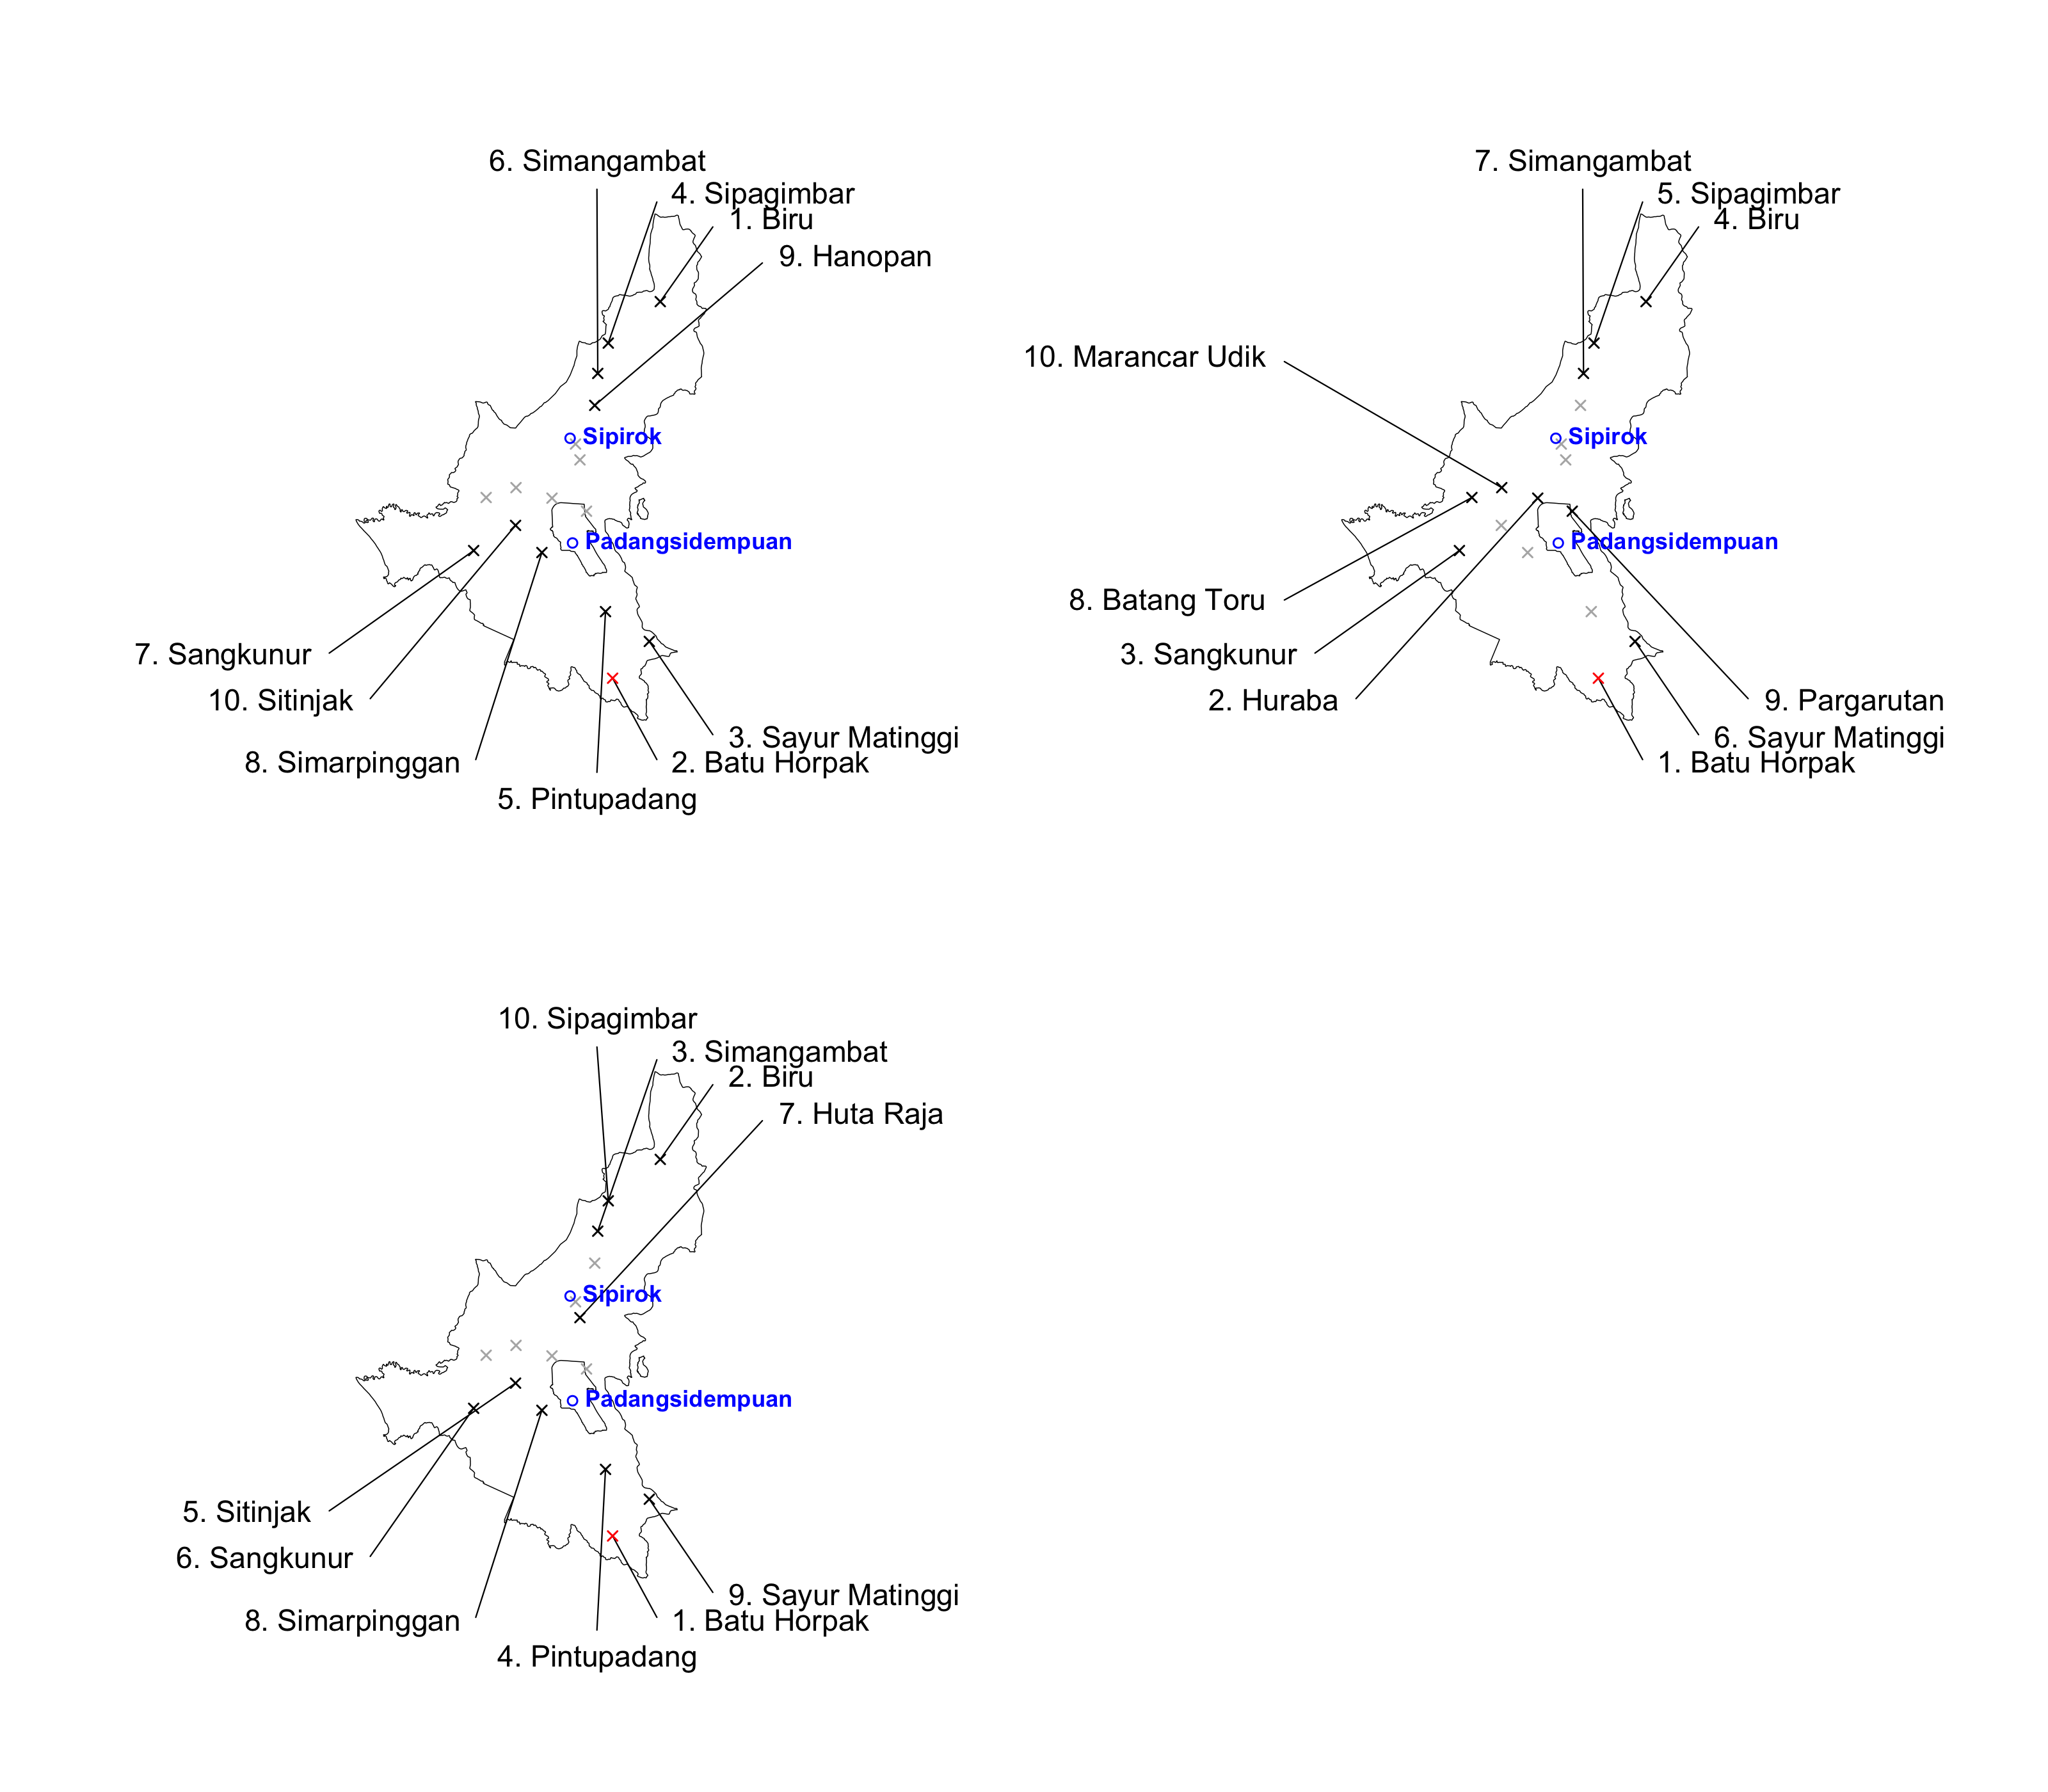
\includegraphics[width=\textwidth]{figs/tapanuli_selatan_all_rank_map.png}
\caption{Mapped best ranked sites in Tapanuli Selatan using catchment definitions of (a) distance-based 
  limits of 30 km (Table \ref{tab:tapanuli_selatan_dist}); (b) travel time-based limits of 100 
  minutes (Table \ref{tab:tapanuli_selatan_time}); and (c) tesselated catchments (Table 
  \ref{tab:tapanuli_selatan_stretch}). Site with ranks shaded in grey were suggested by surveillance study stakeholders. 
 Eco-constraints are indicated in green (pass) and purple (fail), summarised as ``Eco-constraints Present''.}
\label{fig:maps_tapanuli_selatan}
\end{figure}
\clearpage
\subsubsection{Tapanuli Tengah}
% latex table generated in R 4.3.1 by xtable 1.8-4 package
% Wed Sep  4 16:11:51 2024
\begin{table}[ht]
\centering
\begingroup\fontsize{8pt}{9pt}\selectfont
\begin{tabular}{C{0.03\textwidth}C{0.12\textwidth}C{0.09\textwidth}C{0.08\textwidth}C{0.08\textwidth}C{0.08\textwidth}C{0.07\textwidth}C{0.07\textwidth}C{0.07\textwidth}C{0.07\textwidth}}
 Rank & Name & Catchment Size & Objective Mean & Objective Std Dev & Eco-constraints  Present & Human Pop & Croplands & Oil Palm & Forest Loss \\ 
 {1} & Saragih &  93 & \cellcolor[HTML]{BD0026}\textcolor[HTML]{FFFFFF}{0.95} & \cellcolor[HTML]{BD0026}\textcolor[HTML]{FFFFFF}{0.47} & \cellcolor[HTML]{BD0026}\textcolor[HTML]{FFFFFF}{4} & \cellcolor[HTML]{90EE90}{******} & \cellcolor[HTML]{90EE90}{ 1.00} & \cellcolor[HTML]{90EE90}{37.00} & \cellcolor[HTML]{90EE90}{0.29} \\ 
  {2} & Manduamas &  83 & \cellcolor[HTML]{E31A1C}\textcolor[HTML]{FFFFFF}{0.90} & \cellcolor[HTML]{E31A1C}\textcolor[HTML]{FFFFFF}{0.45} & \cellcolor[HTML]{FED976}\textcolor[HTML]{000000}{3} & \cellcolor[HTML]{90EE90}{******} & \cellcolor[HTML]{9370D8}{ 0.00} & \cellcolor[HTML]{90EE90}{37.00} & \cellcolor[HTML]{90EE90}{0.24} \\ 
  {3} & Sirandorung &  79 & \cellcolor[HTML]{FC4E2A}\textcolor[HTML]{000000}{0.85} & \cellcolor[HTML]{FD8D3C}\textcolor[HTML]{000000}{0.40} & \cellcolor[HTML]{FED976}\textcolor[HTML]{000000}{3} & \cellcolor[HTML]{90EE90}{******} & \cellcolor[HTML]{9370D8}{ 0.00} & \cellcolor[HTML]{90EE90}{37.00} & \cellcolor[HTML]{90EE90}{0.24} \\ 
  {4} & Kolang &  87 & \cellcolor[HTML]{FD8D3C}\textcolor[HTML]{000000}{0.82} & \cellcolor[HTML]{FED976}\textcolor[HTML]{000000}{0.34} & \cellcolor[HTML]{FED976}\textcolor[HTML]{000000}{3} & \cellcolor[HTML]{90EE90}{******} & \cellcolor[HTML]{9370D8}{ 0.00} & \cellcolor[HTML]{90EE90}{37.00} & \cellcolor[HTML]{90EE90}{0.12} \\ 
  {5} & Andam Dewi &  81 & \cellcolor[HTML]{FD8D3C}\textcolor[HTML]{000000}{0.82} & \cellcolor[HTML]{FD8D3C}\textcolor[HTML]{000000}{0.40} & \cellcolor[HTML]{FED976}\textcolor[HTML]{000000}{3} & \cellcolor[HTML]{90EE90}{******} & \cellcolor[HTML]{9370D8}{ 0.00} & \cellcolor[HTML]{90EE90}{37.00} & \cellcolor[HTML]{90EE90}{0.24} \\ 
  {6} & Sorkam &  81 & \cellcolor[HTML]{FD8D3C}\textcolor[HTML]{000000}{0.81} & \cellcolor[HTML]{FED976}\textcolor[HTML]{000000}{0.36} & \cellcolor[HTML]{FED976}\textcolor[HTML]{000000}{3} & \cellcolor[HTML]{90EE90}{******} & \cellcolor[HTML]{9370D8}{ 0.00} & \cellcolor[HTML]{90EE90}{37.00} & \cellcolor[HTML]{90EE90}{0.05} \\ 
  {7} & Sipeapea &  78 & \cellcolor[HTML]{FD8D3C}\textcolor[HTML]{000000}{0.79} & \cellcolor[HTML]{FED976}\textcolor[HTML]{000000}{0.36} & \cellcolor[HTML]{FED976}\textcolor[HTML]{000000}{3} & \cellcolor[HTML]{90EE90}{******} & \cellcolor[HTML]{9370D8}{ 0.00} & \cellcolor[HTML]{90EE90}{37.00} & \cellcolor[HTML]{90EE90}{0.05} \\ 
  \cellcolor{lightgray}{8} & Poriaha &  86 & \cellcolor[HTML]{FEB24C}\textcolor[HTML]{000000}{0.79} & \cellcolor[HTML]{FD8D3C}\textcolor[HTML]{000000}{0.39} & \cellcolor[HTML]{FED976}\textcolor[HTML]{000000}{3} & \cellcolor[HTML]{90EE90}{******} & \cellcolor[HTML]{9370D8}{ 0.00} & \cellcolor[HTML]{90EE90}{35.73} & \cellcolor[HTML]{90EE90}{0.05} \\ 
  {9} & Pasaribu Tobing &  98 & \cellcolor[HTML]{FEB24C}\textcolor[HTML]{000000}{0.79} & \cellcolor[HTML]{FED976}\textcolor[HTML]{000000}{0.34} & \cellcolor[HTML]{FED976}\textcolor[HTML]{000000}{3} & \cellcolor[HTML]{90EE90}{******} & \cellcolor[HTML]{9370D8}{ 0.00} & \cellcolor[HTML]{90EE90}{37.00} & \cellcolor[HTML]{90EE90}{0.12} \\ 
  {10} & Siantar Ca &  88 & \cellcolor[HTML]{FEB24C}\textcolor[HTML]{000000}{0.78} & \cellcolor[HTML]{FED976}\textcolor[HTML]{000000}{0.36} & \cellcolor[HTML]{FED976}\textcolor[HTML]{000000}{3} & \cellcolor[HTML]{90EE90}{******} & \cellcolor[HTML]{9370D8}{ 0.00} & \cellcolor[HTML]{90EE90}{37.00} & \cellcolor[HTML]{90EE90}{0.12} \\ 
  {-} & Sibabangun & 113 & \cellcolor[HTML]{FEB24C}\textcolor[HTML]{000000}{0.78} & \cellcolor[HTML]{BD0026}\textcolor[HTML]{FFFFFF}{0.45} & \cellcolor[HTML]{FED976}\textcolor[HTML]{000000}{3} & \cellcolor[HTML]{90EE90}{******} & \cellcolor[HTML]{9370D8}{ 0.00} & \cellcolor[HTML]{90EE90}{37.00} & \cellcolor[HTML]{90EE90}{0.06} \\ 
  {-} & Barus &  72 & \cellcolor[HTML]{FEB24C}\textcolor[HTML]{000000}{0.77} & \cellcolor[HTML]{FD8D3C}\textcolor[HTML]{000000}{0.40} & \cellcolor[HTML]{FED976}\textcolor[HTML]{000000}{3} & \cellcolor[HTML]{90EE90}{******} & \cellcolor[HTML]{9370D8}{ 0.00} & \cellcolor[HTML]{90EE90}{37.00} & \cellcolor[HTML]{90EE90}{0.24} \\ 
  {-} & Sarudik &  93 & \cellcolor[HTML]{FEB24C}\textcolor[HTML]{000000}{0.77} & \cellcolor[HTML]{FC4E2A}\textcolor[HTML]{000000}{0.42} & \cellcolor[HTML]{FED976}\textcolor[HTML]{000000}{3} & \cellcolor[HTML]{90EE90}{******} & \cellcolor[HTML]{9370D8}{ 0.00} & \cellcolor[HTML]{90EE90}{37.00} & \cellcolor[HTML]{90EE90}{0.05} \\ 
  {-} & Pandan & 101 & \cellcolor[HTML]{FEB24C}\textcolor[HTML]{000000}{0.76} & \cellcolor[HTML]{FC4E2A}\textcolor[HTML]{000000}{0.41} & \cellcolor[HTML]{FED976}\textcolor[HTML]{000000}{3} & \cellcolor[HTML]{90EE90}{******} & \cellcolor[HTML]{9370D8}{ 0.00} & \cellcolor[HTML]{90EE90}{37.00} & \cellcolor[HTML]{90EE90}{0.05} \\ 
  {-} & Lumut & 108 & \cellcolor[HTML]{FEB24C}\textcolor[HTML]{000000}{0.75} & \cellcolor[HTML]{FC4E2A}\textcolor[HTML]{000000}{0.42} & \cellcolor[HTML]{FED976}\textcolor[HTML]{000000}{3} & \cellcolor[HTML]{90EE90}{******} & \cellcolor[HTML]{9370D8}{ 0.00} & \cellcolor[HTML]{90EE90}{37.00} & \cellcolor[HTML]{90EE90}{0.06} \\ 
  {-} & Kalangan &  94 & \cellcolor[HTML]{FED976}\textcolor[HTML]{000000}{0.73} & \cellcolor[HTML]{FC4E2A}\textcolor[HTML]{000000}{0.42} & \cellcolor[HTML]{FED976}\textcolor[HTML]{000000}{3} & \cellcolor[HTML]{90EE90}{******} & \cellcolor[HTML]{9370D8}{ 0.00} & \cellcolor[HTML]{90EE90}{37.00} & \cellcolor[HTML]{90EE90}{0.05} \\ 
  {-} & Pinangsori & 102 & \cellcolor[HTML]{FED976}\textcolor[HTML]{000000}{0.72} & \cellcolor[HTML]{FC4E2A}\textcolor[HTML]{000000}{0.42} & \cellcolor[HTML]{FED976}\textcolor[HTML]{000000}{3} & \cellcolor[HTML]{90EE90}{******} & \cellcolor[HTML]{9370D8}{ 0.00} & \cellcolor[HTML]{90EE90}{37.00} & \cellcolor[HTML]{90EE90}{0.06} \\ 
  {-} & Aek Raisan & 107 & \cellcolor[HTML]{FED976}\textcolor[HTML]{000000}{0.72} & \cellcolor[HTML]{FEB24C}\textcolor[HTML]{000000}{0.36} & \cellcolor[HTML]{BD0026}\textcolor[HTML]{FFFFFF}{4} & \cellcolor[HTML]{90EE90}{******} & \cellcolor[HTML]{90EE90}{18.94} & \cellcolor[HTML]{90EE90}{37.00} & \cellcolor[HTML]{90EE90}{0.05} \\ 
  {-} & Badiri &  94 & \cellcolor[HTML]{FED976}\textcolor[HTML]{000000}{0.71} & \cellcolor[HTML]{FC4E2A}\textcolor[HTML]{000000}{0.42} & \cellcolor[HTML]{FED976}\textcolor[HTML]{000000}{3} & \cellcolor[HTML]{90EE90}{******} & \cellcolor[HTML]{9370D8}{ 0.00} & \cellcolor[HTML]{90EE90}{37.00} & \cellcolor[HTML]{90EE90}{0.05} \\ 
  \end{tabular}
\endgroup
\caption{Tapanuli Tengah sites (distance catchments, 30 km)} 
\label{tab:tapanuli_tengah_dist}
\end{table}
% latex table generated in R 4.3.1 by xtable 1.8-4 package
% Wed Sep  4 16:11:51 2024
\begin{table}[ht]
\centering
\begingroup\fontsize{8pt}{9pt}\selectfont
\begin{tabular}{C{0.03\textwidth}C{0.12\textwidth}C{0.09\textwidth}C{0.08\textwidth}C{0.08\textwidth}C{0.08\textwidth}C{0.07\textwidth}C{0.07\textwidth}C{0.07\textwidth}C{0.07\textwidth}}
 Rank & Name & Catchment Size & Objective Mean & Objective Std Dev & Eco-constraints  Present & Human Pop & Croplands & Oil Palm & Forest Loss \\ 
 {1} & Saragih &  15 & \cellcolor[HTML]{BD0026}\textcolor[HTML]{FFFFFF}{0.85} & \cellcolor[HTML]{BD0026}\textcolor[HTML]{FFFFFF}{0.41} & \cellcolor[HTML]{FED976}\textcolor[HTML]{000000}{3} & \cellcolor[HTML]{90EE90}{*****} & \cellcolor[HTML]{9370D8}{ 0.00} & \cellcolor[HTML]{90EE90}{36.42} & \cellcolor[HTML]{90EE90}{0.09} \\ 
  {2} & Sipeapea &  50 & \cellcolor[HTML]{E31A1C}\textcolor[HTML]{FFFFFF}{0.72} & \cellcolor[HTML]{BD0026}\textcolor[HTML]{FFFFFF}{0.44} & \cellcolor[HTML]{BD0026}\textcolor[HTML]{FFFFFF}{4} & \cellcolor[HTML]{90EE90}{******} & \cellcolor[HTML]{90EE90}{18.94} & \cellcolor[HTML]{90EE90}{37.00} & \cellcolor[HTML]{90EE90}{0.05} \\ 
  {3} & Sorkam &  60 & \cellcolor[HTML]{E31A1C}\textcolor[HTML]{FFFFFF}{0.69} & \cellcolor[HTML]{BD0026}\textcolor[HTML]{FFFFFF}{0.42} & \cellcolor[HTML]{BD0026}\textcolor[HTML]{FFFFFF}{4} & \cellcolor[HTML]{90EE90}{******} & \cellcolor[HTML]{90EE90}{18.94} & \cellcolor[HTML]{90EE90}{37.00} & \cellcolor[HTML]{90EE90}{0.05} \\ 
  {4} & Siantar Ca &  28 & \cellcolor[HTML]{FC4E2A}\textcolor[HTML]{000000}{0.69} & \cellcolor[HTML]{E31A1C}\textcolor[HTML]{FFFFFF}{0.40} & \cellcolor[HTML]{FED976}\textcolor[HTML]{000000}{3} & \cellcolor[HTML]{90EE90}{******} & \cellcolor[HTML]{9370D8}{ 0.00} & \cellcolor[HTML]{90EE90}{37.00} & \cellcolor[HTML]{90EE90}{0.06} \\ 
  {5} & Kolang & 111 & \cellcolor[HTML]{FC4E2A}\textcolor[HTML]{000000}{0.61} & \cellcolor[HTML]{FC4E2A}\textcolor[HTML]{000000}{0.36} & \cellcolor[HTML]{BD0026}\textcolor[HTML]{FFFFFF}{4} & \cellcolor[HTML]{90EE90}{******} & \cellcolor[HTML]{90EE90}{18.96} & \cellcolor[HTML]{90EE90}{37.00} & \cellcolor[HTML]{90EE90}{0.10} \\ 
  {6} & Sibabangun & 310 & \cellcolor[HTML]{FD8D3C}\textcolor[HTML]{000000}{0.58} & \cellcolor[HTML]{FD8D3C}\textcolor[HTML]{000000}{0.33} & \cellcolor[HTML]{BD0026}\textcolor[HTML]{FFFFFF}{4} & \cellcolor[HTML]{90EE90}{*******} & \cellcolor[HTML]{90EE90}{60.83} & \cellcolor[HTML]{90EE90}{37.00} & \cellcolor[HTML]{90EE90}{0.22} \\ 
  {7} & Lumut & 309 & \cellcolor[HTML]{FD8D3C}\textcolor[HTML]{000000}{0.57} & \cellcolor[HTML]{FD8D3C}\textcolor[HTML]{000000}{0.33} & \cellcolor[HTML]{BD0026}\textcolor[HTML]{FFFFFF}{4} & \cellcolor[HTML]{90EE90}{*******} & \cellcolor[HTML]{90EE90}{60.83} & \cellcolor[HTML]{90EE90}{37.00} & \cellcolor[HTML]{90EE90}{0.22} \\ 
  {8} & Pinangsori & 314 & \cellcolor[HTML]{FD8D3C}\textcolor[HTML]{000000}{0.57} & \cellcolor[HTML]{FD8D3C}\textcolor[HTML]{000000}{0.33} & \cellcolor[HTML]{BD0026}\textcolor[HTML]{FFFFFF}{4} & \cellcolor[HTML]{90EE90}{*******} & \cellcolor[HTML]{90EE90}{60.83} & \cellcolor[HTML]{90EE90}{37.00} & \cellcolor[HTML]{90EE90}{0.22} \\ 
  \cellcolor{lightgray}{9} & Poriaha & 282 & \cellcolor[HTML]{FD8D3C}\textcolor[HTML]{000000}{0.56} & \cellcolor[HTML]{FEB24C}\textcolor[HTML]{000000}{0.31} & \cellcolor[HTML]{BD0026}\textcolor[HTML]{FFFFFF}{4} & \cellcolor[HTML]{90EE90}{*******} & \cellcolor[HTML]{90EE90}{60.83} & \cellcolor[HTML]{90EE90}{37.00} & \cellcolor[HTML]{90EE90}{0.14} \\ 
  {10} & Aek Raisan & 313 & \cellcolor[HTML]{FD8D3C}\textcolor[HTML]{000000}{0.55} & \cellcolor[HTML]{FEB24C}\textcolor[HTML]{000000}{0.30} & \cellcolor[HTML]{BD0026}\textcolor[HTML]{FFFFFF}{4} & \cellcolor[HTML]{90EE90}{*******} & \cellcolor[HTML]{90EE90}{60.83} & \cellcolor[HTML]{90EE90}{37.00} & \cellcolor[HTML]{90EE90}{0.14} \\ 
  {-} & Badiri & 319 & \cellcolor[HTML]{FD8D3C}\textcolor[HTML]{000000}{0.55} & \cellcolor[HTML]{FEB24C}\textcolor[HTML]{000000}{0.31} & \cellcolor[HTML]{BD0026}\textcolor[HTML]{FFFFFF}{4} & \cellcolor[HTML]{90EE90}{*******} & \cellcolor[HTML]{90EE90}{60.83} & \cellcolor[HTML]{90EE90}{37.00} & \cellcolor[HTML]{90EE90}{0.22} \\ 
  {-} & Sarudik & 310 & \cellcolor[HTML]{FD8D3C}\textcolor[HTML]{000000}{0.55} & \cellcolor[HTML]{FEB24C}\textcolor[HTML]{000000}{0.31} & \cellcolor[HTML]{BD0026}\textcolor[HTML]{FFFFFF}{4} & \cellcolor[HTML]{90EE90}{*******} & \cellcolor[HTML]{90EE90}{60.83} & \cellcolor[HTML]{90EE90}{37.00} & \cellcolor[HTML]{90EE90}{0.14} \\ 
  {-} & Pandan & 268 & \cellcolor[HTML]{FD8D3C}\textcolor[HTML]{000000}{0.54} & \cellcolor[HTML]{FD8D3C}\textcolor[HTML]{000000}{0.32} & \cellcolor[HTML]{BD0026}\textcolor[HTML]{FFFFFF}{4} & \cellcolor[HTML]{90EE90}{*******} & \cellcolor[HTML]{90EE90}{60.83} & \cellcolor[HTML]{90EE90}{37.00} & \cellcolor[HTML]{90EE90}{0.14} \\ 
  {-} & Kalangan & 316 & \cellcolor[HTML]{FD8D3C}\textcolor[HTML]{000000}{0.54} & \cellcolor[HTML]{FEB24C}\textcolor[HTML]{000000}{0.31} & \cellcolor[HTML]{BD0026}\textcolor[HTML]{FFFFFF}{4} & \cellcolor[HTML]{90EE90}{*******} & \cellcolor[HTML]{90EE90}{60.83} & \cellcolor[HTML]{90EE90}{37.00} & \cellcolor[HTML]{90EE90}{0.22} \\ 
  {-} & Andam Dewi &  27 & \cellcolor[HTML]{FD8D3C}\textcolor[HTML]{000000}{0.54} & \cellcolor[HTML]{FD8D3C}\textcolor[HTML]{000000}{0.32} & \cellcolor[HTML]{FED976}\textcolor[HTML]{000000}{3} & \cellcolor[HTML]{90EE90}{******} & \cellcolor[HTML]{9370D8}{ 0.00} & \cellcolor[HTML]{90EE90}{37.00} & \cellcolor[HTML]{90EE90}{0.08} \\ 
  {-} & Barus &  25 & \cellcolor[HTML]{FEB24C}\textcolor[HTML]{000000}{0.51} & \cellcolor[HTML]{FD8D3C}\textcolor[HTML]{000000}{0.31} & \cellcolor[HTML]{FED976}\textcolor[HTML]{000000}{3} & \cellcolor[HTML]{90EE90}{******} & \cellcolor[HTML]{9370D8}{ 0.00} & \cellcolor[HTML]{90EE90}{37.00} & \cellcolor[HTML]{90EE90}{0.08} \\ 
  {-} & Sirandorung &  19 & \cellcolor[HTML]{FEB24C}\textcolor[HTML]{000000}{0.48} & \cellcolor[HTML]{FD8D3C}\textcolor[HTML]{000000}{0.33} & \cellcolor[HTML]{FED976}\textcolor[HTML]{000000}{3} & \cellcolor[HTML]{90EE90}{*****} & \cellcolor[HTML]{9370D8}{ 0.00} & \cellcolor[HTML]{90EE90}{37.00} & \cellcolor[HTML]{90EE90}{0.24} \\ 
  {-} & Manduamas &  15 & \cellcolor[HTML]{FED976}\textcolor[HTML]{000000}{0.41} & \cellcolor[HTML]{FD8D3C}\textcolor[HTML]{000000}{0.33} & \cellcolor[HTML]{FED976}\textcolor[HTML]{000000}{3} & \cellcolor[HTML]{90EE90}{*****} & \cellcolor[HTML]{9370D8}{ 0.00} & \cellcolor[HTML]{90EE90}{37.00} & \cellcolor[HTML]{90EE90}{0.24} \\ 
  {-} & Pasaribu Tobing &   4 & \cellcolor[HTML]{FED976}\textcolor[HTML]{000000}{0.38} & \cellcolor[HTML]{FED976}\textcolor[HTML]{000000}{0.25} & \cellcolor[HTML]{FED976}\textcolor[HTML]{000000}{3} & \cellcolor[HTML]{90EE90}{*****} & \cellcolor[HTML]{9370D8}{ 0.00} & \cellcolor[HTML]{90EE90}{35.21} & \cellcolor[HTML]{90EE90}{0.05} \\ 
  \end{tabular}
\endgroup
\caption{Tapanuli Tengah sites (travel time catchments, 100 minutes)} 
\label{tab:tapanuli_tengah_time}
\end{table}
% latex table generated in R 4.3.1 by xtable 1.8-4 package
% Wed Sep  4 16:11:51 2024
\begin{table}[ht]
\centering
\begingroup\fontsize{8pt}{9pt}\selectfont
\begin{tabular}{C{0.03\textwidth}C{0.12\textwidth}C{0.09\textwidth}C{0.08\textwidth}C{0.08\textwidth}C{0.08\textwidth}C{0.07\textwidth}C{0.07\textwidth}C{0.07\textwidth}C{0.07\textwidth}}
 Rank & Name & Catchment Size & Objective Mean & Objective Std Dev & Eco-constraints  Present & Human Pop & Croplands & Oil Palm & Forest Loss \\ 
 {1} & Pasaribu Tobing &   7 & \cellcolor[HTML]{BD0026}\textcolor[HTML]{FFFFFF}{1.21} & \cellcolor[HTML]{FC4E2A}\textcolor[HTML]{000000}{0.44} & \cellcolor[HTML]{BD0026}\textcolor[HTML]{FFFFFF}{3} & \cellcolor[HTML]{90EE90}{*****} & \cellcolor[HTML]{9370D8}{0} & \cellcolor[HTML]{90EE90}{35.13} & \cellcolor[HTML]{90EE90}{0.05} \\ 
  {2} & Lumut &   7 & \cellcolor[HTML]{E31A1C}\textcolor[HTML]{FFFFFF}{1.03} & \cellcolor[HTML]{E31A1C}\textcolor[HTML]{FFFFFF}{0.45} & \cellcolor[HTML]{BD0026}\textcolor[HTML]{FFFFFF}{3} & \cellcolor[HTML]{90EE90}{*****} & \cellcolor[HTML]{9370D8}{0} & \cellcolor[HTML]{90EE90}{37.00} & \cellcolor[HTML]{90EE90}{0.03} \\ 
  {3} & Badiri &   8 & \cellcolor[HTML]{E31A1C}\textcolor[HTML]{FFFFFF}{1.00} & \cellcolor[HTML]{BD0026}\textcolor[HTML]{FFFFFF}{0.63} & \cellcolor[HTML]{BD0026}\textcolor[HTML]{FFFFFF}{3} & \cellcolor[HTML]{90EE90}{*****} & \cellcolor[HTML]{9370D8}{0} & \cellcolor[HTML]{90EE90}{34.93} & \cellcolor[HTML]{90EE90}{0.02} \\ 
  {4} & Sibabangun &   5 & \cellcolor[HTML]{E31A1C}\textcolor[HTML]{FFFFFF}{0.92} & \cellcolor[HTML]{BD0026}\textcolor[HTML]{FFFFFF}{0.60} & \cellcolor[HTML]{BD0026}\textcolor[HTML]{FFFFFF}{3} & \cellcolor[HTML]{90EE90}{*****} & \cellcolor[HTML]{9370D8}{0} & \cellcolor[HTML]{90EE90}{37.00} & \cellcolor[HTML]{90EE90}{0.03} \\ 
  {5} & Aek Raisan &   8 & \cellcolor[HTML]{FC4E2A}\textcolor[HTML]{000000}{0.88} & \cellcolor[HTML]{FEB24C}\textcolor[HTML]{000000}{0.23} & \cellcolor[HTML]{BD0026}\textcolor[HTML]{FFFFFF}{3} & \cellcolor[HTML]{90EE90}{*****} & \cellcolor[HTML]{9370D8}{0} & \cellcolor[HTML]{90EE90}{24.95} & \cellcolor[HTML]{90EE90}{0.01} \\ 
  {6} & Pinangsori &   9 & \cellcolor[HTML]{FC4E2A}\textcolor[HTML]{000000}{0.83} & \cellcolor[HTML]{E31A1C}\textcolor[HTML]{FFFFFF}{0.52} & \cellcolor[HTML]{BD0026}\textcolor[HTML]{FFFFFF}{3} & \cellcolor[HTML]{90EE90}{*****} & \cellcolor[HTML]{9370D8}{0} & \cellcolor[HTML]{90EE90}{27.93} & \cellcolor[HTML]{90EE90}{0.02} \\ 
  {7} & Siantar Ca &   9 & \cellcolor[HTML]{FC4E2A}\textcolor[HTML]{000000}{0.80} & \cellcolor[HTML]{FD8D3C}\textcolor[HTML]{000000}{0.32} & \cellcolor[HTML]{BD0026}\textcolor[HTML]{FFFFFF}{3} & \cellcolor[HTML]{90EE90}{*****} & \cellcolor[HTML]{9370D8}{0} & \cellcolor[HTML]{90EE90}{33.72} & \cellcolor[HTML]{90EE90}{0.03} \\ 
  {8} & Kolang &   9 & \cellcolor[HTML]{FC4E2A}\textcolor[HTML]{000000}{0.79} & \cellcolor[HTML]{FC4E2A}\textcolor[HTML]{000000}{0.43} & \cellcolor[HTML]{BD0026}\textcolor[HTML]{FFFFFF}{3} & \cellcolor[HTML]{90EE90}{*****} & \cellcolor[HTML]{9370D8}{0} & \cellcolor[HTML]{90EE90}{33.25} & \cellcolor[HTML]{90EE90}{0.05} \\ 
  {9} & Saragih &   6 & \cellcolor[HTML]{FC4E2A}\textcolor[HTML]{000000}{0.79} & \cellcolor[HTML]{FC4E2A}\textcolor[HTML]{000000}{0.42} & \cellcolor[HTML]{BD0026}\textcolor[HTML]{FFFFFF}{3} & \cellcolor[HTML]{90EE90}{*****} & \cellcolor[HTML]{9370D8}{0} & \cellcolor[HTML]{90EE90}{32.40} & \cellcolor[HTML]{90EE90}{0.05} \\ 
  {10} & Andam Dewi &   5 & \cellcolor[HTML]{FD8D3C}\textcolor[HTML]{000000}{0.72} & \cellcolor[HTML]{FC4E2A}\textcolor[HTML]{000000}{0.35} & \cellcolor[HTML]{BD0026}\textcolor[HTML]{FFFFFF}{3} & \cellcolor[HTML]{90EE90}{*****} & \cellcolor[HTML]{9370D8}{0} & \cellcolor[HTML]{90EE90}{36.27} & \cellcolor[HTML]{90EE90}{0.04} \\ 
  \cellcolor{lightgray}{-} & Poriaha &   8 & \cellcolor[HTML]{FD8D3C}\textcolor[HTML]{000000}{0.70} & \cellcolor[HTML]{FEB24C}\textcolor[HTML]{000000}{0.25} & \cellcolor[HTML]{BD0026}\textcolor[HTML]{FFFFFF}{3} & \cellcolor[HTML]{90EE90}{*****} & \cellcolor[HTML]{9370D8}{0} & \cellcolor[HTML]{90EE90}{30.78} & \cellcolor[HTML]{90EE90}{0.01} \\ 
  {-} & Sarudik &   2 & \cellcolor[HTML]{FD8D3C}\textcolor[HTML]{000000}{0.67} & \cellcolor[HTML]{FED976}\textcolor[HTML]{000000}{0.07} & \cellcolor[HTML]{BD0026}\textcolor[HTML]{FFFFFF}{3} & \cellcolor[HTML]{90EE90}{*****} & \cellcolor[HTML]{9370D8}{0} & \cellcolor[HTML]{90EE90}{24.17} & \cellcolor[HTML]{90EE90}{0.01} \\ 
  {-} & Pandan &   8 & \cellcolor[HTML]{FD8D3C}\textcolor[HTML]{000000}{0.60} & \cellcolor[HTML]{FD8D3C}\textcolor[HTML]{000000}{0.34} & \cellcolor[HTML]{BD0026}\textcolor[HTML]{FFFFFF}{3} & \cellcolor[HTML]{90EE90}{*****} & \cellcolor[HTML]{9370D8}{0} & \cellcolor[HTML]{90EE90}{35.73} & \cellcolor[HTML]{90EE90}{0.01} \\ 
  {-} & Sorkam &   4 & \cellcolor[HTML]{FEB24C}\textcolor[HTML]{000000}{0.57} & \cellcolor[HTML]{E31A1C}\textcolor[HTML]{FFFFFF}{0.45} & \cellcolor[HTML]{BD0026}\textcolor[HTML]{FFFFFF}{3} & \cellcolor[HTML]{90EE90}{*****} & \cellcolor[HTML]{9370D8}{0} & \cellcolor[HTML]{90EE90}{33.69} & \cellcolor[HTML]{90EE90}{0.01} \\ 
  {-} & Sirandorung &   6 & \cellcolor[HTML]{FEB24C}\textcolor[HTML]{000000}{0.48} & \cellcolor[HTML]{FC4E2A}\textcolor[HTML]{000000}{0.40} & \cellcolor[HTML]{BD0026}\textcolor[HTML]{FFFFFF}{3} & \cellcolor[HTML]{90EE90}{*****} & \cellcolor[HTML]{9370D8}{0} & \cellcolor[HTML]{90EE90}{37.00} & \cellcolor[HTML]{90EE90}{0.08} \\ 
  {-} & Kalangan &   1 & \cellcolor[HTML]{FEB24C}\textcolor[HTML]{000000}{0.46} & \cellcolor[HTML]{FFFFFF}\textcolor[HTML]{000000}{  NA} & \cellcolor[HTML]{FED976}\textcolor[HTML]{000000}{2} & \cellcolor[HTML]{9370D8}{****} & \cellcolor[HTML]{9370D8}{0} & \cellcolor[HTML]{90EE90}{35.36} & \cellcolor[HTML]{90EE90}{0.01} \\ 
  {-} & Barus &   2 & \cellcolor[HTML]{FED976}\textcolor[HTML]{000000}{0.42} & \cellcolor[HTML]{E31A1C}\textcolor[HTML]{FFFFFF}{0.48} & \cellcolor[HTML]{BD0026}\textcolor[HTML]{FFFFFF}{3} & \cellcolor[HTML]{90EE90}{*****} & \cellcolor[HTML]{9370D8}{0} & \cellcolor[HTML]{90EE90}{37.00} & \cellcolor[HTML]{90EE90}{0.01} \\ 
  {-} & Sipeapea &   2 & \cellcolor[HTML]{FED976}\textcolor[HTML]{000000}{0.41} & \cellcolor[HTML]{FD8D3C}\textcolor[HTML]{000000}{0.35} & \cellcolor[HTML]{BD0026}\textcolor[HTML]{FFFFFF}{3} & \cellcolor[HTML]{90EE90}{*****} & \cellcolor[HTML]{9370D8}{0} & \cellcolor[HTML]{90EE90}{35.21} & \cellcolor[HTML]{90EE90}{0.02} \\ 
  {-} & Manduamas &   6 & \cellcolor[HTML]{FED976}\textcolor[HTML]{000000}{0.29} & \cellcolor[HTML]{FEB24C}\textcolor[HTML]{000000}{0.22} & \cellcolor[HTML]{BD0026}\textcolor[HTML]{FFFFFF}{3} & \cellcolor[HTML]{90EE90}{*****} & \cellcolor[HTML]{9370D8}{0} & \cellcolor[HTML]{90EE90}{37.00} & \cellcolor[HTML]{90EE90}{0.24} \\ 
  \end{tabular}
\endgroup
\caption{Tapanuli Tengah sites (``closest point'' catchments)} 
\label{tab:tapanuli_tengah_stretch}
\end{table}
\begin{figure}
\centering
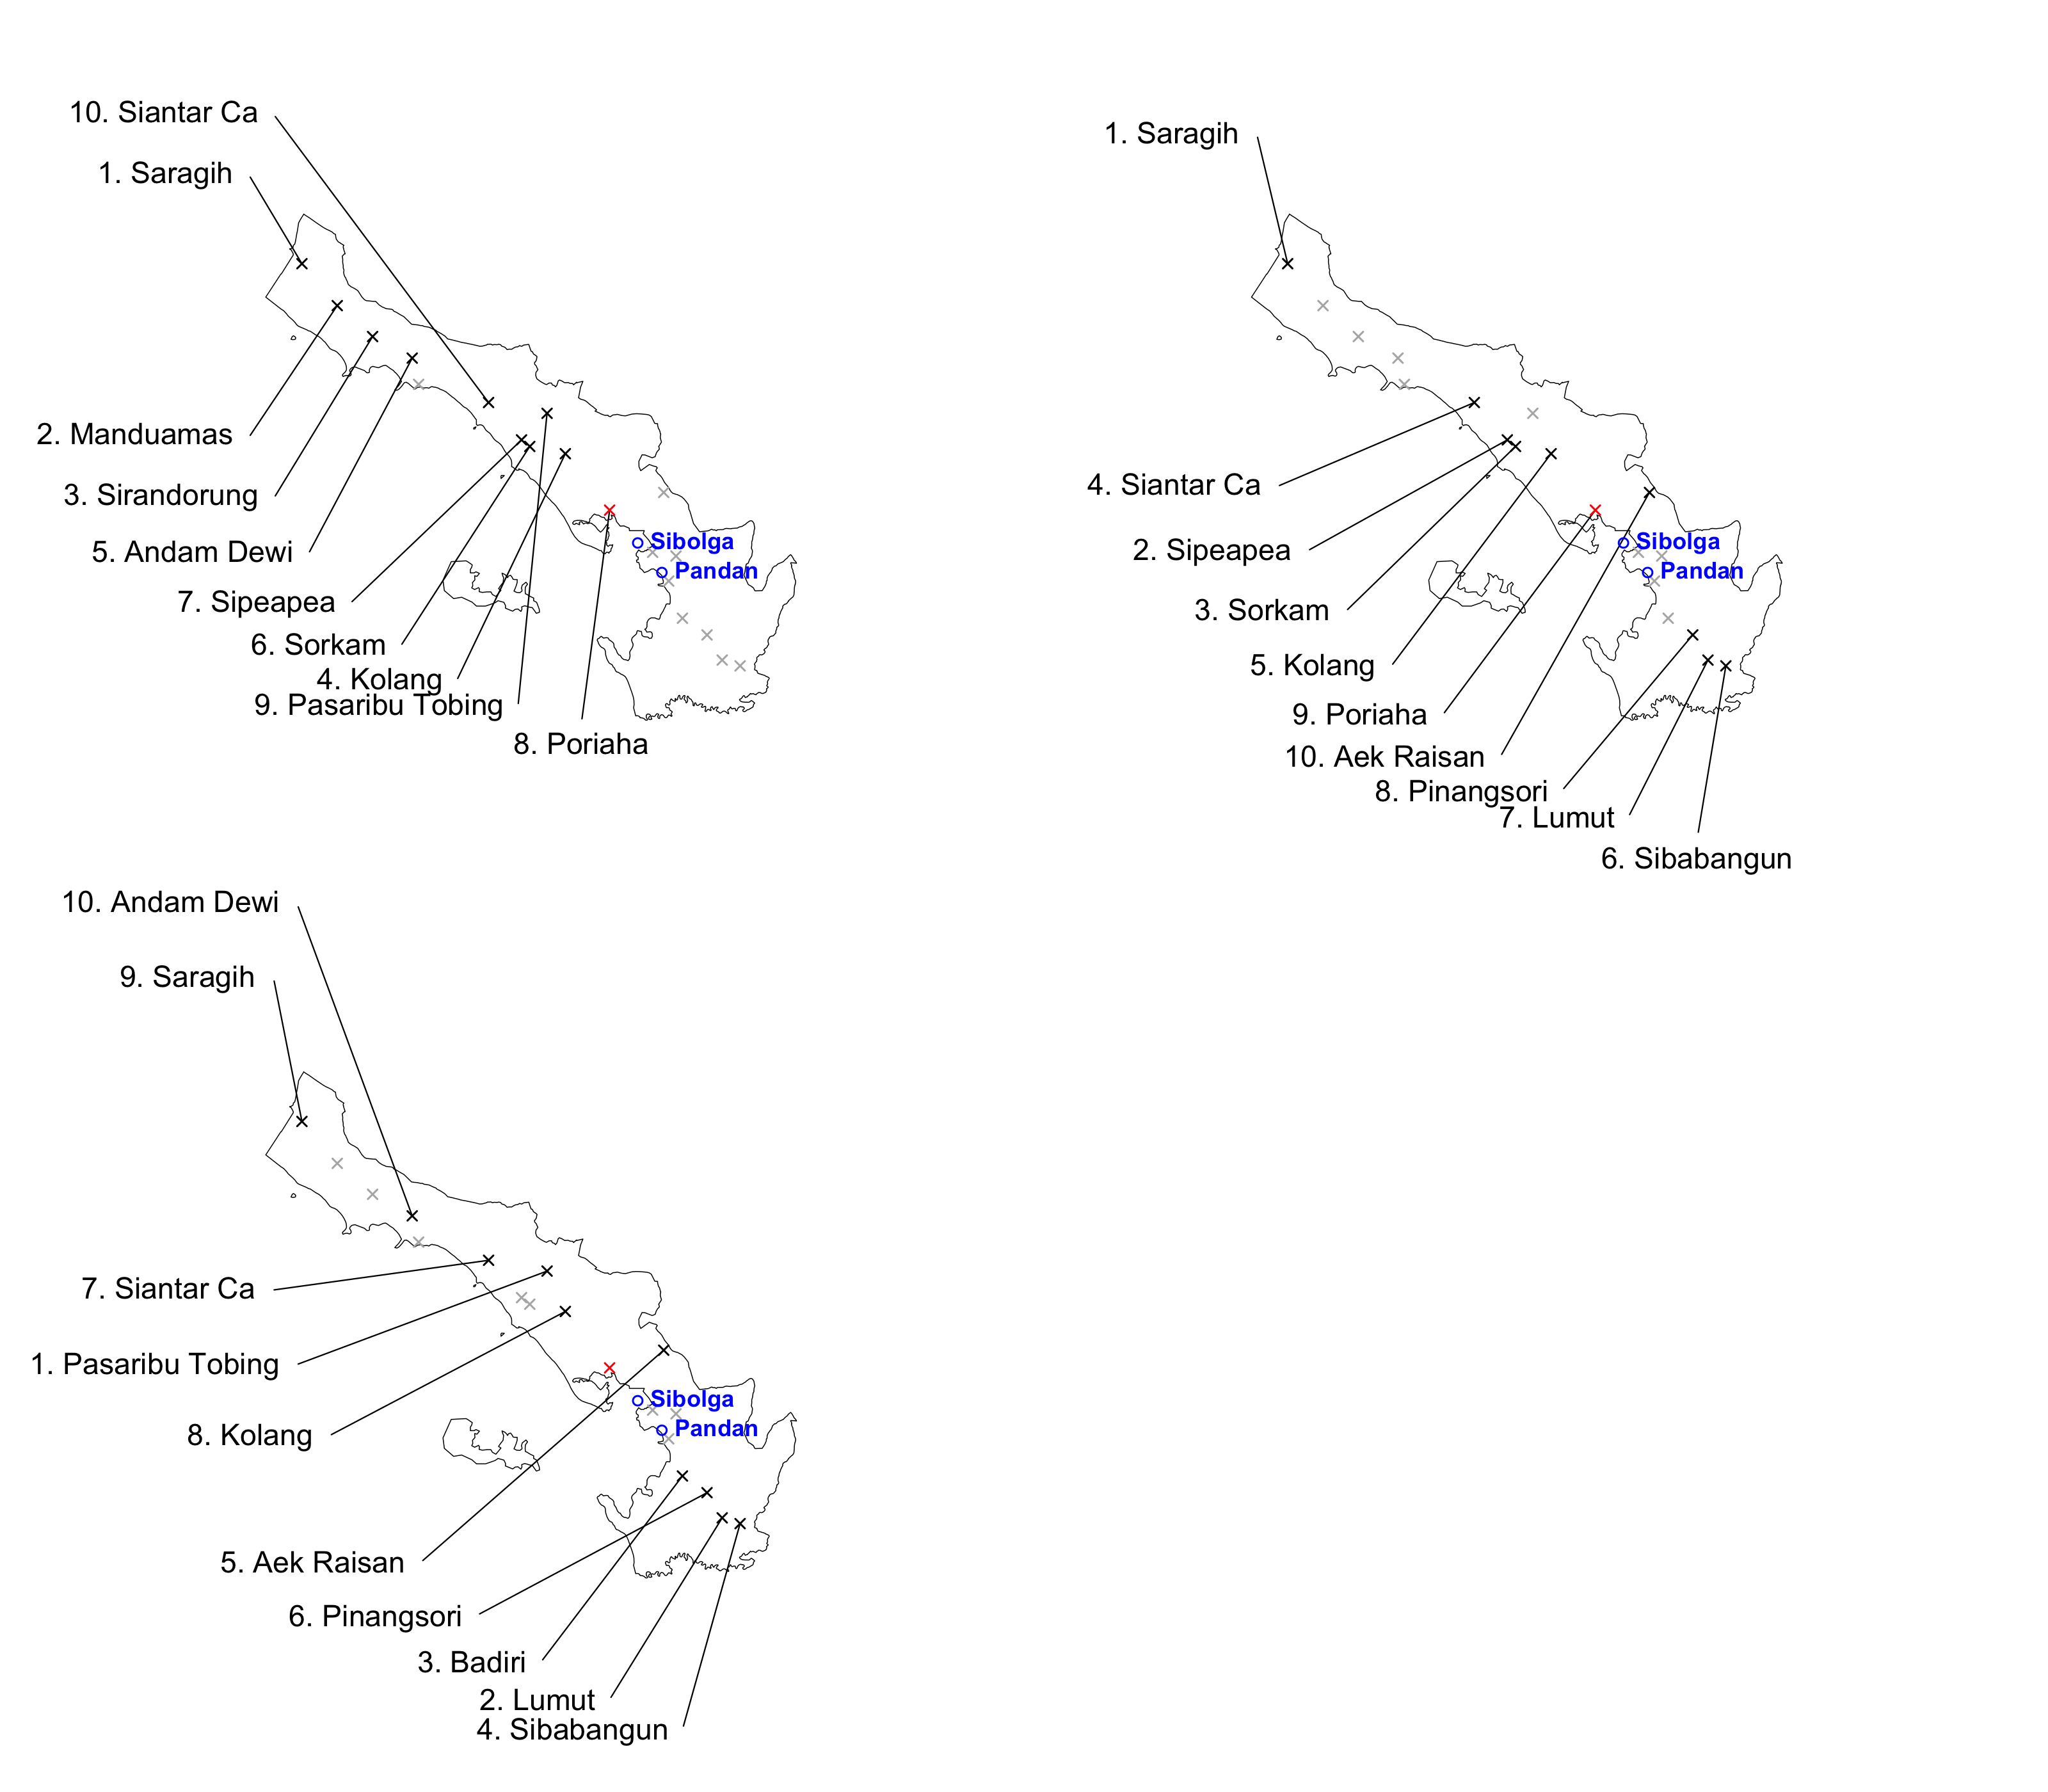
\includegraphics[width=\textwidth]{figs/tapanuli_tengah_all_rank_map.png}
\caption{Mapped best ranked sites in Tapanuli Tengah using catchment definitions of (a) distance-based 
  limits of 30 km (Table \ref{tab:tapanuli_tengah_dist}); (b) travel time-based limits of 100 
  minutes (Table \ref{tab:tapanuli_tengah_time}); and (c) tesselated catchments (Table 
  \ref{tab:tapanuli_tengah_stretch}). Site with ranks shaded in grey were suggested by surveillance study stakeholders. 
 Eco-constraints are indicated in green (pass) and purple (fail), summarised as ``Eco-constraints Present''.}
\label{fig:maps_tapanuli_tengah}
\end{figure}
\clearpage
\subsubsection{Dairi}
% latex table generated in R 4.3.1 by xtable 1.8-4 package
% Wed Sep  4 16:11:51 2024
\begin{table}[ht]
\centering
\begingroup\fontsize{8pt}{9pt}\selectfont
\begin{tabular}{C{0.03\textwidth}C{0.12\textwidth}C{0.09\textwidth}C{0.08\textwidth}C{0.08\textwidth}C{0.08\textwidth}C{0.07\textwidth}C{0.07\textwidth}C{0.07\textwidth}C{0.07\textwidth}}
 Rank & Name & Catchment Size & Objective Mean & Objective Std Dev & Eco-constraints  Present & Human Pop & Croplands & Oil Palm & Forest Loss \\ 
 {1} & Sopobutar & 130 & \cellcolor[HTML]{BD0026}\textcolor[HTML]{FFFFFF}{0.91} & \cellcolor[HTML]{BD0026}\textcolor[HTML]{FFFFFF}{0.58} & \cellcolor[HTML]{FD8D3C}\textcolor[HTML]{000000}{4} & \cellcolor[HTML]{90EE90}{******} & \cellcolor[HTML]{90EE90}{27.97} & \cellcolor[HTML]{90EE90}{37} & \cellcolor[HTML]{90EE90}{0.28} \\ 
  {2} & Parongil & 132 & \cellcolor[HTML]{BD0026}\textcolor[HTML]{FFFFFF}{0.88} & \cellcolor[HTML]{BD0026}\textcolor[HTML]{FFFFFF}{0.58} & \cellcolor[HTML]{FD8D3C}\textcolor[HTML]{000000}{4} & \cellcolor[HTML]{90EE90}{******} & \cellcolor[HTML]{90EE90}{19.94} & \cellcolor[HTML]{90EE90}{37} & \cellcolor[HTML]{90EE90}{0.28} \\ 
  {3} & Bakal Gajah & 135 & \cellcolor[HTML]{BD0026}\textcolor[HTML]{FFFFFF}{0.86} & \cellcolor[HTML]{BD0026}\textcolor[HTML]{FFFFFF}{0.58} & \cellcolor[HTML]{FD8D3C}\textcolor[HTML]{000000}{4} & \cellcolor[HTML]{90EE90}{******} & \cellcolor[HTML]{90EE90}{27.97} & \cellcolor[HTML]{90EE90}{37} & \cellcolor[HTML]{90EE90}{0.28} \\ 
  {4} & Buntu Raja & 133 & \cellcolor[HTML]{E31A1C}\textcolor[HTML]{FFFFFF}{0.81} & \cellcolor[HTML]{BD0026}\textcolor[HTML]{FFFFFF}{0.54} & \cellcolor[HTML]{FD8D3C}\textcolor[HTML]{000000}{4} & \cellcolor[HTML]{90EE90}{******} & \cellcolor[HTML]{90EE90}{19.94} & \cellcolor[HTML]{90EE90}{37} & \cellcolor[HTML]{90EE90}{0.28} \\ 
  {5} & Kentara & 135 & \cellcolor[HTML]{E31A1C}\textcolor[HTML]{FFFFFF}{0.79} & \cellcolor[HTML]{FC4E2A}\textcolor[HTML]{000000}{0.49} & \cellcolor[HTML]{FD8D3C}\textcolor[HTML]{000000}{4} & \cellcolor[HTML]{90EE90}{******} & \cellcolor[HTML]{90EE90}{11.96} & \cellcolor[HTML]{90EE90}{37} & \cellcolor[HTML]{90EE90}{0.28} \\ 
  {6} & Berampu & 129 & \cellcolor[HTML]{FC4E2A}\textcolor[HTML]{000000}{0.77} & \cellcolor[HTML]{FC4E2A}\textcolor[HTML]{000000}{0.45} & \cellcolor[HTML]{FD8D3C}\textcolor[HTML]{000000}{4} & \cellcolor[HTML]{90EE90}{******} & \cellcolor[HTML]{90EE90}{11.96} & \cellcolor[HTML]{90EE90}{37} & \cellcolor[HTML]{90EE90}{0.28} \\ 
  {7} & Batang Beruh & 129 & \cellcolor[HTML]{FC4E2A}\textcolor[HTML]{000000}{0.76} & \cellcolor[HTML]{FD8D3C}\textcolor[HTML]{000000}{0.44} & \cellcolor[HTML]{FD8D3C}\textcolor[HTML]{000000}{4} & \cellcolor[HTML]{90EE90}{******} & \cellcolor[HTML]{90EE90}{11.96} & \cellcolor[HTML]{90EE90}{37} & \cellcolor[HTML]{90EE90}{0.03} \\ 
  {8} & Huta Rakyat & 128 & \cellcolor[HTML]{FC4E2A}\textcolor[HTML]{000000}{0.76} & \cellcolor[HTML]{FC4E2A}\textcolor[HTML]{000000}{0.45} & \cellcolor[HTML]{FD8D3C}\textcolor[HTML]{000000}{4} & \cellcolor[HTML]{90EE90}{******} & \cellcolor[HTML]{90EE90}{11.96} & \cellcolor[HTML]{90EE90}{37} & \cellcolor[HTML]{90EE90}{0.05} \\ 
  {9} & Sitinjo & 127 & \cellcolor[HTML]{FC4E2A}\textcolor[HTML]{000000}{0.73} & \cellcolor[HTML]{FD8D3C}\textcolor[HTML]{000000}{0.43} & \cellcolor[HTML]{FD8D3C}\textcolor[HTML]{000000}{4} & \cellcolor[HTML]{90EE90}{******} & \cellcolor[HTML]{90EE90}{11.96} & \cellcolor[HTML]{90EE90}{37} & \cellcolor[HTML]{90EE90}{0.03} \\ 
  {10} & Sigalingging & 125 & \cellcolor[HTML]{FC4E2A}\textcolor[HTML]{000000}{0.73} & \cellcolor[HTML]{FD8D3C}\textcolor[HTML]{000000}{0.42} & \cellcolor[HTML]{FD8D3C}\textcolor[HTML]{000000}{4} & \cellcolor[HTML]{90EE90}{******} & \cellcolor[HTML]{90EE90}{ 3.99} & \cellcolor[HTML]{90EE90}{37} & \cellcolor[HTML]{90EE90}{0.03} \\ 
  {-} & Tiga Lingga & 130 & \cellcolor[HTML]{FD8D3C}\textcolor[HTML]{000000}{0.68} & \cellcolor[HTML]{E31A1C}\textcolor[HTML]{FFFFFF}{0.51} & \cellcolor[HTML]{FD8D3C}\textcolor[HTML]{000000}{4} & \cellcolor[HTML]{90EE90}{******} & \cellcolor[HTML]{90EE90}{27.97} & \cellcolor[HTML]{90EE90}{37} & \cellcolor[HTML]{90EE90}{0.28} \\ 
  \cellcolor{lightgray}{-} & Kilometer 11 & 130 & \cellcolor[HTML]{FD8D3C}\textcolor[HTML]{000000}{0.68} & \cellcolor[HTML]{FC4E2A}\textcolor[HTML]{000000}{0.45} & \cellcolor[HTML]{FD8D3C}\textcolor[HTML]{000000}{4} & \cellcolor[HTML]{90EE90}{******} & \cellcolor[HTML]{90EE90}{19.94} & \cellcolor[HTML]{90EE90}{37} & \cellcolor[HTML]{90EE90}{0.28} \\ 
  {-} & Pegagan Julu Ii & 124 & \cellcolor[HTML]{FEB24C}\textcolor[HTML]{000000}{0.63} & \cellcolor[HTML]{FEB24C}\textcolor[HTML]{000000}{0.40} & \cellcolor[HTML]{FD8D3C}\textcolor[HTML]{000000}{4} & \cellcolor[HTML]{90EE90}{******} & \cellcolor[HTML]{90EE90}{11.96} & \cellcolor[HTML]{90EE90}{37} & \cellcolor[HTML]{90EE90}{0.13} \\ 
  {-} & Tiga Baru & 124 & \cellcolor[HTML]{FEB24C}\textcolor[HTML]{000000}{0.60} & \cellcolor[HTML]{FEB24C}\textcolor[HTML]{000000}{0.38} & \cellcolor[HTML]{FD8D3C}\textcolor[HTML]{000000}{4} & \cellcolor[HTML]{90EE90}{******} & \cellcolor[HTML]{90EE90}{11.96} & \cellcolor[HTML]{90EE90}{37} & \cellcolor[HTML]{90EE90}{0.13} \\ 
  {-} & Silalahi & 124 & \cellcolor[HTML]{FED976}\textcolor[HTML]{000000}{0.51} & \cellcolor[HTML]{FED976}\textcolor[HTML]{000000}{0.31} & \cellcolor[HTML]{FD8D3C}\textcolor[HTML]{000000}{4} & \cellcolor[HTML]{90EE90}{******} & \cellcolor[HTML]{90EE90}{ 5.98} & \cellcolor[HTML]{90EE90}{37} & \cellcolor[HTML]{90EE90}{0.13} \\ 
  \end{tabular}
\endgroup
\caption{Dairi sites (distance catchments, 30 km)} 
\label{tab:dairi_dist}
\end{table}
% latex table generated in R 4.3.1 by xtable 1.8-4 package
% Wed Sep  4 16:11:51 2024
\begin{table}[ht]
\centering
\begingroup\fontsize{8pt}{9pt}\selectfont
\begin{tabular}{C{0.03\textwidth}C{0.12\textwidth}C{0.09\textwidth}C{0.08\textwidth}C{0.08\textwidth}C{0.08\textwidth}C{0.07\textwidth}C{0.07\textwidth}C{0.07\textwidth}C{0.07\textwidth}}
 Rank & Name & Catchment Size & Objective Mean & Objective Std Dev & Eco-constraints  Present & Human Pop & Croplands & Oil Palm & Forest Loss \\ 
 \cellcolor{lightgray}{1} & Kilometer 11 & 249 & \cellcolor[HTML]{BD0026}\textcolor[HTML]{FFFFFF}{0.50} & \cellcolor[HTML]{E31A1C}\textcolor[HTML]{FFFFFF}{0.38} & \cellcolor[HTML]{FD8D3C}\textcolor[HTML]{000000}{4} & \cellcolor[HTML]{90EE90}{*******} & \cellcolor[HTML]{90EE90}{61.91} & \cellcolor[HTML]{90EE90}{37} & \cellcolor[HTML]{90EE90}{0.13} \\ 
  {2} & Berampu & 239 & \cellcolor[HTML]{BD0026}\textcolor[HTML]{FFFFFF}{0.49} & \cellcolor[HTML]{E31A1C}\textcolor[HTML]{FFFFFF}{0.39} & \cellcolor[HTML]{FD8D3C}\textcolor[HTML]{000000}{4} & \cellcolor[HTML]{90EE90}{*******} & \cellcolor[HTML]{90EE90}{61.91} & \cellcolor[HTML]{90EE90}{37} & \cellcolor[HTML]{90EE90}{0.13} \\ 
  {3} & Kentara & 197 & \cellcolor[HTML]{BD0026}\textcolor[HTML]{FFFFFF}{0.49} & \cellcolor[HTML]{E31A1C}\textcolor[HTML]{FFFFFF}{0.37} & \cellcolor[HTML]{FD8D3C}\textcolor[HTML]{000000}{4} & \cellcolor[HTML]{90EE90}{******} & \cellcolor[HTML]{90EE90}{61.91} & \cellcolor[HTML]{90EE90}{37} & \cellcolor[HTML]{90EE90}{0.13} \\ 
  {4} & Huta Rakyat & 311 & \cellcolor[HTML]{E31A1C}\textcolor[HTML]{FFFFFF}{0.47} & \cellcolor[HTML]{BD0026}\textcolor[HTML]{FFFFFF}{0.40} & \cellcolor[HTML]{FD8D3C}\textcolor[HTML]{000000}{4} & \cellcolor[HTML]{90EE90}{*******} & \cellcolor[HTML]{90EE90}{67.95} & \cellcolor[HTML]{90EE90}{37} & \cellcolor[HTML]{90EE90}{0.13} \\ 
  {5} & Batang Beruh & 367 & \cellcolor[HTML]{FC4E2A}\textcolor[HTML]{000000}{0.46} & \cellcolor[HTML]{BD0026}\textcolor[HTML]{FFFFFF}{0.41} & \cellcolor[HTML]{FD8D3C}\textcolor[HTML]{000000}{4} & \cellcolor[HTML]{90EE90}{*******} & \cellcolor[HTML]{90EE90}{76.89} & \cellcolor[HTML]{90EE90}{37} & \cellcolor[HTML]{90EE90}{0.13} \\ 
  {6} & Buntu Raja & 166 & \cellcolor[HTML]{FC4E2A}\textcolor[HTML]{000000}{0.46} & \cellcolor[HTML]{FC4E2A}\textcolor[HTML]{000000}{0.35} & \cellcolor[HTML]{FD8D3C}\textcolor[HTML]{000000}{4} & \cellcolor[HTML]{90EE90}{******} & \cellcolor[HTML]{90EE90}{61.91} & \cellcolor[HTML]{90EE90}{37} & \cellcolor[HTML]{90EE90}{0.13} \\ 
  {7} & Tiga Baru & 221 & \cellcolor[HTML]{FC4E2A}\textcolor[HTML]{000000}{0.46} & \cellcolor[HTML]{E31A1C}\textcolor[HTML]{FFFFFF}{0.37} & \cellcolor[HTML]{FD8D3C}\textcolor[HTML]{000000}{4} & \cellcolor[HTML]{90EE90}{*******} & \cellcolor[HTML]{90EE90}{61.91} & \cellcolor[HTML]{90EE90}{37} & \cellcolor[HTML]{90EE90}{0.13} \\ 
  {8} & Sigalingging & 196 & \cellcolor[HTML]{FC4E2A}\textcolor[HTML]{000000}{0.45} & \cellcolor[HTML]{FD8D3C}\textcolor[HTML]{000000}{0.34} & \cellcolor[HTML]{FD8D3C}\textcolor[HTML]{000000}{4} & \cellcolor[HTML]{90EE90}{*******} & \cellcolor[HTML]{90EE90}{61.91} & \cellcolor[HTML]{90EE90}{37} & \cellcolor[HTML]{90EE90}{0.13} \\ 
  {9} & Tiga Lingga & 236 & \cellcolor[HTML]{FD8D3C}\textcolor[HTML]{000000}{0.44} & \cellcolor[HTML]{FC4E2A}\textcolor[HTML]{000000}{0.35} & \cellcolor[HTML]{FD8D3C}\textcolor[HTML]{000000}{4} & \cellcolor[HTML]{90EE90}{*******} & \cellcolor[HTML]{90EE90}{61.91} & \cellcolor[HTML]{90EE90}{37} & \cellcolor[HTML]{90EE90}{0.13} \\ 
  {10} & Sitinjo & 366 & \cellcolor[HTML]{FD8D3C}\textcolor[HTML]{000000}{0.44} & \cellcolor[HTML]{BD0026}\textcolor[HTML]{FFFFFF}{0.40} & \cellcolor[HTML]{FD8D3C}\textcolor[HTML]{000000}{4} & \cellcolor[HTML]{90EE90}{*******} & \cellcolor[HTML]{90EE90}{94.86} & \cellcolor[HTML]{90EE90}{37} & \cellcolor[HTML]{90EE90}{0.13} \\ 
  {-} & Sopobutar &  55 & \cellcolor[HTML]{FD8D3C}\textcolor[HTML]{000000}{0.43} & \cellcolor[HTML]{FED976}\textcolor[HTML]{000000}{0.29} & \cellcolor[HTML]{FD8D3C}\textcolor[HTML]{000000}{4} & \cellcolor[HTML]{90EE90}{******} & \cellcolor[HTML]{90EE90}{61.91} & \cellcolor[HTML]{90EE90}{37} & \cellcolor[HTML]{90EE90}{0.04} \\ 
  {-} & Pegagan Julu Ii & 400 & \cellcolor[HTML]{FEB24C}\textcolor[HTML]{000000}{0.43} & \cellcolor[HTML]{E31A1C}\textcolor[HTML]{FFFFFF}{0.38} & \cellcolor[HTML]{FD8D3C}\textcolor[HTML]{000000}{4} & \cellcolor[HTML]{90EE90}{*******} & \cellcolor[HTML]{90EE90}{94.86} & \cellcolor[HTML]{90EE90}{37} & \cellcolor[HTML]{90EE90}{0.13} \\ 
  {-} & Bakal Gajah & 105 & \cellcolor[HTML]{FEB24C}\textcolor[HTML]{000000}{0.42} & \cellcolor[HTML]{FEB24C}\textcolor[HTML]{000000}{0.32} & \cellcolor[HTML]{FD8D3C}\textcolor[HTML]{000000}{4} & \cellcolor[HTML]{90EE90}{******} & \cellcolor[HTML]{90EE90}{61.91} & \cellcolor[HTML]{90EE90}{37} & \cellcolor[HTML]{90EE90}{0.04} \\ 
  {-} & Parongil & 115 & \cellcolor[HTML]{FEB24C}\textcolor[HTML]{000000}{0.41} & \cellcolor[HTML]{FEB24C}\textcolor[HTML]{000000}{0.31} & \cellcolor[HTML]{FD8D3C}\textcolor[HTML]{000000}{4} & \cellcolor[HTML]{90EE90}{******} & \cellcolor[HTML]{90EE90}{61.91} & \cellcolor[HTML]{90EE90}{37} & \cellcolor[HTML]{90EE90}{0.13} \\ 
  {-} & Silalahi & 334 & \cellcolor[HTML]{FED976}\textcolor[HTML]{000000}{0.39} & \cellcolor[HTML]{FC4E2A}\textcolor[HTML]{000000}{0.36} & \cellcolor[HTML]{FD8D3C}\textcolor[HTML]{000000}{4} & \cellcolor[HTML]{90EE90}{*******} & \cellcolor[HTML]{90EE90}{94.86} & \cellcolor[HTML]{90EE90}{37} & \cellcolor[HTML]{90EE90}{0.13} \\ 
  \end{tabular}
\endgroup
\caption{Dairi sites (travel time catchments, 100 minutes)} 
\label{tab:dairi_time}
\end{table}
% latex table generated in R 4.3.1 by xtable 1.8-4 package
% Wed Sep  4 16:11:51 2024
\begin{table}[ht]
\centering
\begingroup\fontsize{8pt}{9pt}\selectfont
\begin{tabular}{C{0.03\textwidth}C{0.12\textwidth}C{0.09\textwidth}C{0.08\textwidth}C{0.08\textwidth}C{0.08\textwidth}C{0.07\textwidth}C{0.07\textwidth}C{0.07\textwidth}C{0.07\textwidth}}
 Rank & Name & Catchment Size & Objective Mean & Objective Std Dev & Eco-constraints  Present & Human Pop & Croplands & Oil Palm & Forest Loss \\ 
 {1} & Sopobutar &  21 & \cellcolor[HTML]{BD0026}\textcolor[HTML]{FFFFFF}{1.22} & \cellcolor[HTML]{BD0026}\textcolor[HTML]{FFFFFF}{0.49} & \cellcolor[HTML]{BD0026}\textcolor[HTML]{FFFFFF}{4} & \cellcolor[HTML]{90EE90}{*****} & \cellcolor[HTML]{90EE90}{ 6.00} & \cellcolor[HTML]{90EE90}{37.00} & \cellcolor[HTML]{90EE90}{0.10} \\ 
  {2} & Berampu &   3 & \cellcolor[HTML]{FC4E2A}\textcolor[HTML]{000000}{0.78} & \cellcolor[HTML]{BD0026}\textcolor[HTML]{FFFFFF}{0.55} & \cellcolor[HTML]{BD0026}\textcolor[HTML]{FFFFFF}{4} & \cellcolor[HTML]{90EE90}{*****} & \cellcolor[HTML]{90EE90}{ 3.99} & \cellcolor[HTML]{90EE90}{37.00} & \cellcolor[HTML]{90EE90}{0.01} \\ 
  {3} & Sigalingging &  11 & \cellcolor[HTML]{FD8D3C}\textcolor[HTML]{000000}{0.70} & \cellcolor[HTML]{FC4E2A}\textcolor[HTML]{000000}{0.32} & \cellcolor[HTML]{FD8D3C}\textcolor[HTML]{000000}{3} & \cellcolor[HTML]{90EE90}{*****} & \cellcolor[HTML]{9370D8}{ 0.00} & \cellcolor[HTML]{90EE90}{37.00} & \cellcolor[HTML]{90EE90}{0.03} \\ 
  {4} & Parongil &   3 & \cellcolor[HTML]{FD8D3C}\textcolor[HTML]{000000}{0.70} & \cellcolor[HTML]{FC4E2A}\textcolor[HTML]{000000}{0.34} & \cellcolor[HTML]{FED976}\textcolor[HTML]{000000}{2} & \cellcolor[HTML]{9370D8}{****} & \cellcolor[HTML]{9370D8}{ 0.00} & \cellcolor[HTML]{90EE90}{37.00} & \cellcolor[HTML]{90EE90}{0.02} \\ 
  {5} & Silalahi &   8 & \cellcolor[HTML]{FD8D3C}\textcolor[HTML]{000000}{0.64} & \cellcolor[HTML]{FC4E2A}\textcolor[HTML]{000000}{0.34} & \cellcolor[HTML]{BD0026}\textcolor[HTML]{FFFFFF}{4} & \cellcolor[HTML]{90EE90}{*****} & \cellcolor[HTML]{90EE90}{ 1.00} & \cellcolor[HTML]{90EE90}{19.08} & \cellcolor[HTML]{90EE90}{0.02} \\ 
  {6} & Tiga Baru &  10 & \cellcolor[HTML]{FD8D3C}\textcolor[HTML]{000000}{0.60} & \cellcolor[HTML]{FC4E2A}\textcolor[HTML]{000000}{0.33} & \cellcolor[HTML]{BD0026}\textcolor[HTML]{FFFFFF}{4} & \cellcolor[HTML]{90EE90}{*****} & \cellcolor[HTML]{90EE90}{ 0.00} & \cellcolor[HTML]{90EE90}{36.65} & \cellcolor[HTML]{90EE90}{0.03} \\ 
  {7} & Kentara &   2 & \cellcolor[HTML]{FEB24C}\textcolor[HTML]{000000}{0.53} & \cellcolor[HTML]{FC4E2A}\textcolor[HTML]{000000}{0.32} & \cellcolor[HTML]{FD8D3C}\textcolor[HTML]{000000}{3} & \cellcolor[HTML]{9370D8}{****} & \cellcolor[HTML]{90EE90}{ 1.99} & \cellcolor[HTML]{90EE90}{25.56} & \cellcolor[HTML]{90EE90}{0.01} \\ 
  {8} & Sitinjo &   3 & \cellcolor[HTML]{FEB24C}\textcolor[HTML]{000000}{0.48} & \cellcolor[HTML]{FD8D3C}\textcolor[HTML]{000000}{0.22} & \cellcolor[HTML]{FD8D3C}\textcolor[HTML]{000000}{3} & \cellcolor[HTML]{90EE90}{*****} & \cellcolor[HTML]{9370D8}{ 0.00} & \cellcolor[HTML]{90EE90}{37.00} & \cellcolor[HTML]{90EE90}{0.01} \\ 
  {9} & Tiga Lingga &  15 & \cellcolor[HTML]{FEB24C}\textcolor[HTML]{000000}{0.44} & \cellcolor[HTML]{FD8D3C}\textcolor[HTML]{000000}{0.21} & \cellcolor[HTML]{BD0026}\textcolor[HTML]{FFFFFF}{4} & \cellcolor[HTML]{90EE90}{*****} & \cellcolor[HTML]{90EE90}{27.97} & \cellcolor[HTML]{90EE90}{37.00} & \cellcolor[HTML]{90EE90}{0.02} \\ 
  {10} & Bakal Gajah &   2 & \cellcolor[HTML]{FEB24C}\textcolor[HTML]{000000}{0.42} & \cellcolor[HTML]{FEB24C}\textcolor[HTML]{000000}{0.14} & \cellcolor[HTML]{FED976}\textcolor[HTML]{000000}{2} & \cellcolor[HTML]{9370D8}{****} & \cellcolor[HTML]{9370D8}{ 0.00} & \cellcolor[HTML]{90EE90}{37.00} & \cellcolor[HTML]{90EE90}{0.02} \\ 
  \cellcolor{lightgray}{-} & Kilometer 11 &   6 & \cellcolor[HTML]{FED976}\textcolor[HTML]{000000}{0.37} & \cellcolor[HTML]{FD8D3C}\textcolor[HTML]{000000}{0.28} & \cellcolor[HTML]{BD0026}\textcolor[HTML]{FFFFFF}{4} & \cellcolor[HTML]{90EE90}{*****} & \cellcolor[HTML]{90EE90}{ 0.00} & \cellcolor[HTML]{90EE90}{37.00} & \cellcolor[HTML]{90EE90}{0.01} \\ 
  {-} & Pegagan Julu Ii &   4 & \cellcolor[HTML]{FED976}\textcolor[HTML]{000000}{0.30} & \cellcolor[HTML]{FED976}\textcolor[HTML]{000000}{0.10} & \cellcolor[HTML]{FD8D3C}\textcolor[HTML]{000000}{3} & \cellcolor[HTML]{90EE90}{*****} & \cellcolor[HTML]{9370D8}{ 0.00} & \cellcolor[HTML]{90EE90}{36.40} & \cellcolor[HTML]{90EE90}{0.03} \\ 
  {-} & Batang Beruh &   3 & \cellcolor[HTML]{FED976}\textcolor[HTML]{000000}{0.25} & \cellcolor[HTML]{FED976}\textcolor[HTML]{000000}{0.11} & \cellcolor[HTML]{BD0026}\textcolor[HTML]{FFFFFF}{4} & \cellcolor[HTML]{90EE90}{*****} & \cellcolor[HTML]{90EE90}{ 1.00} & \cellcolor[HTML]{90EE90}{36.95} & \cellcolor[HTML]{90EE90}{0.01} \\ 
  {-} & Buntu Raja &   3 & \cellcolor[HTML]{FED976}\textcolor[HTML]{000000}{0.24} & \cellcolor[HTML]{FED976}\textcolor[HTML]{000000}{0.04} & \cellcolor[HTML]{BD0026}\textcolor[HTML]{FFFFFF}{4} & \cellcolor[HTML]{90EE90}{*****} & \cellcolor[HTML]{90EE90}{11.96} & \cellcolor[HTML]{90EE90}{37.00} & \cellcolor[HTML]{90EE90}{0.02} \\ 
  {-} & Huta Rakyat &   1 & \cellcolor[HTML]{FED976}\textcolor[HTML]{000000}{0.20} & \cellcolor[HTML]{FFFFFF}\textcolor[HTML]{000000}{  NA} & \cellcolor[HTML]{BD0026}\textcolor[HTML]{FFFFFF}{4} & \cellcolor[HTML]{90EE90}{*****} & \cellcolor[HTML]{90EE90}{ 0.01} & \cellcolor[HTML]{90EE90}{36.87} & \cellcolor[HTML]{90EE90}{0.00} \\ 
  \end{tabular}
\endgroup
\caption{Dairi sites (``closest point'' catchments)} 
\label{tab:dairi_stretch}
\end{table}
\begin{figure}
\centering
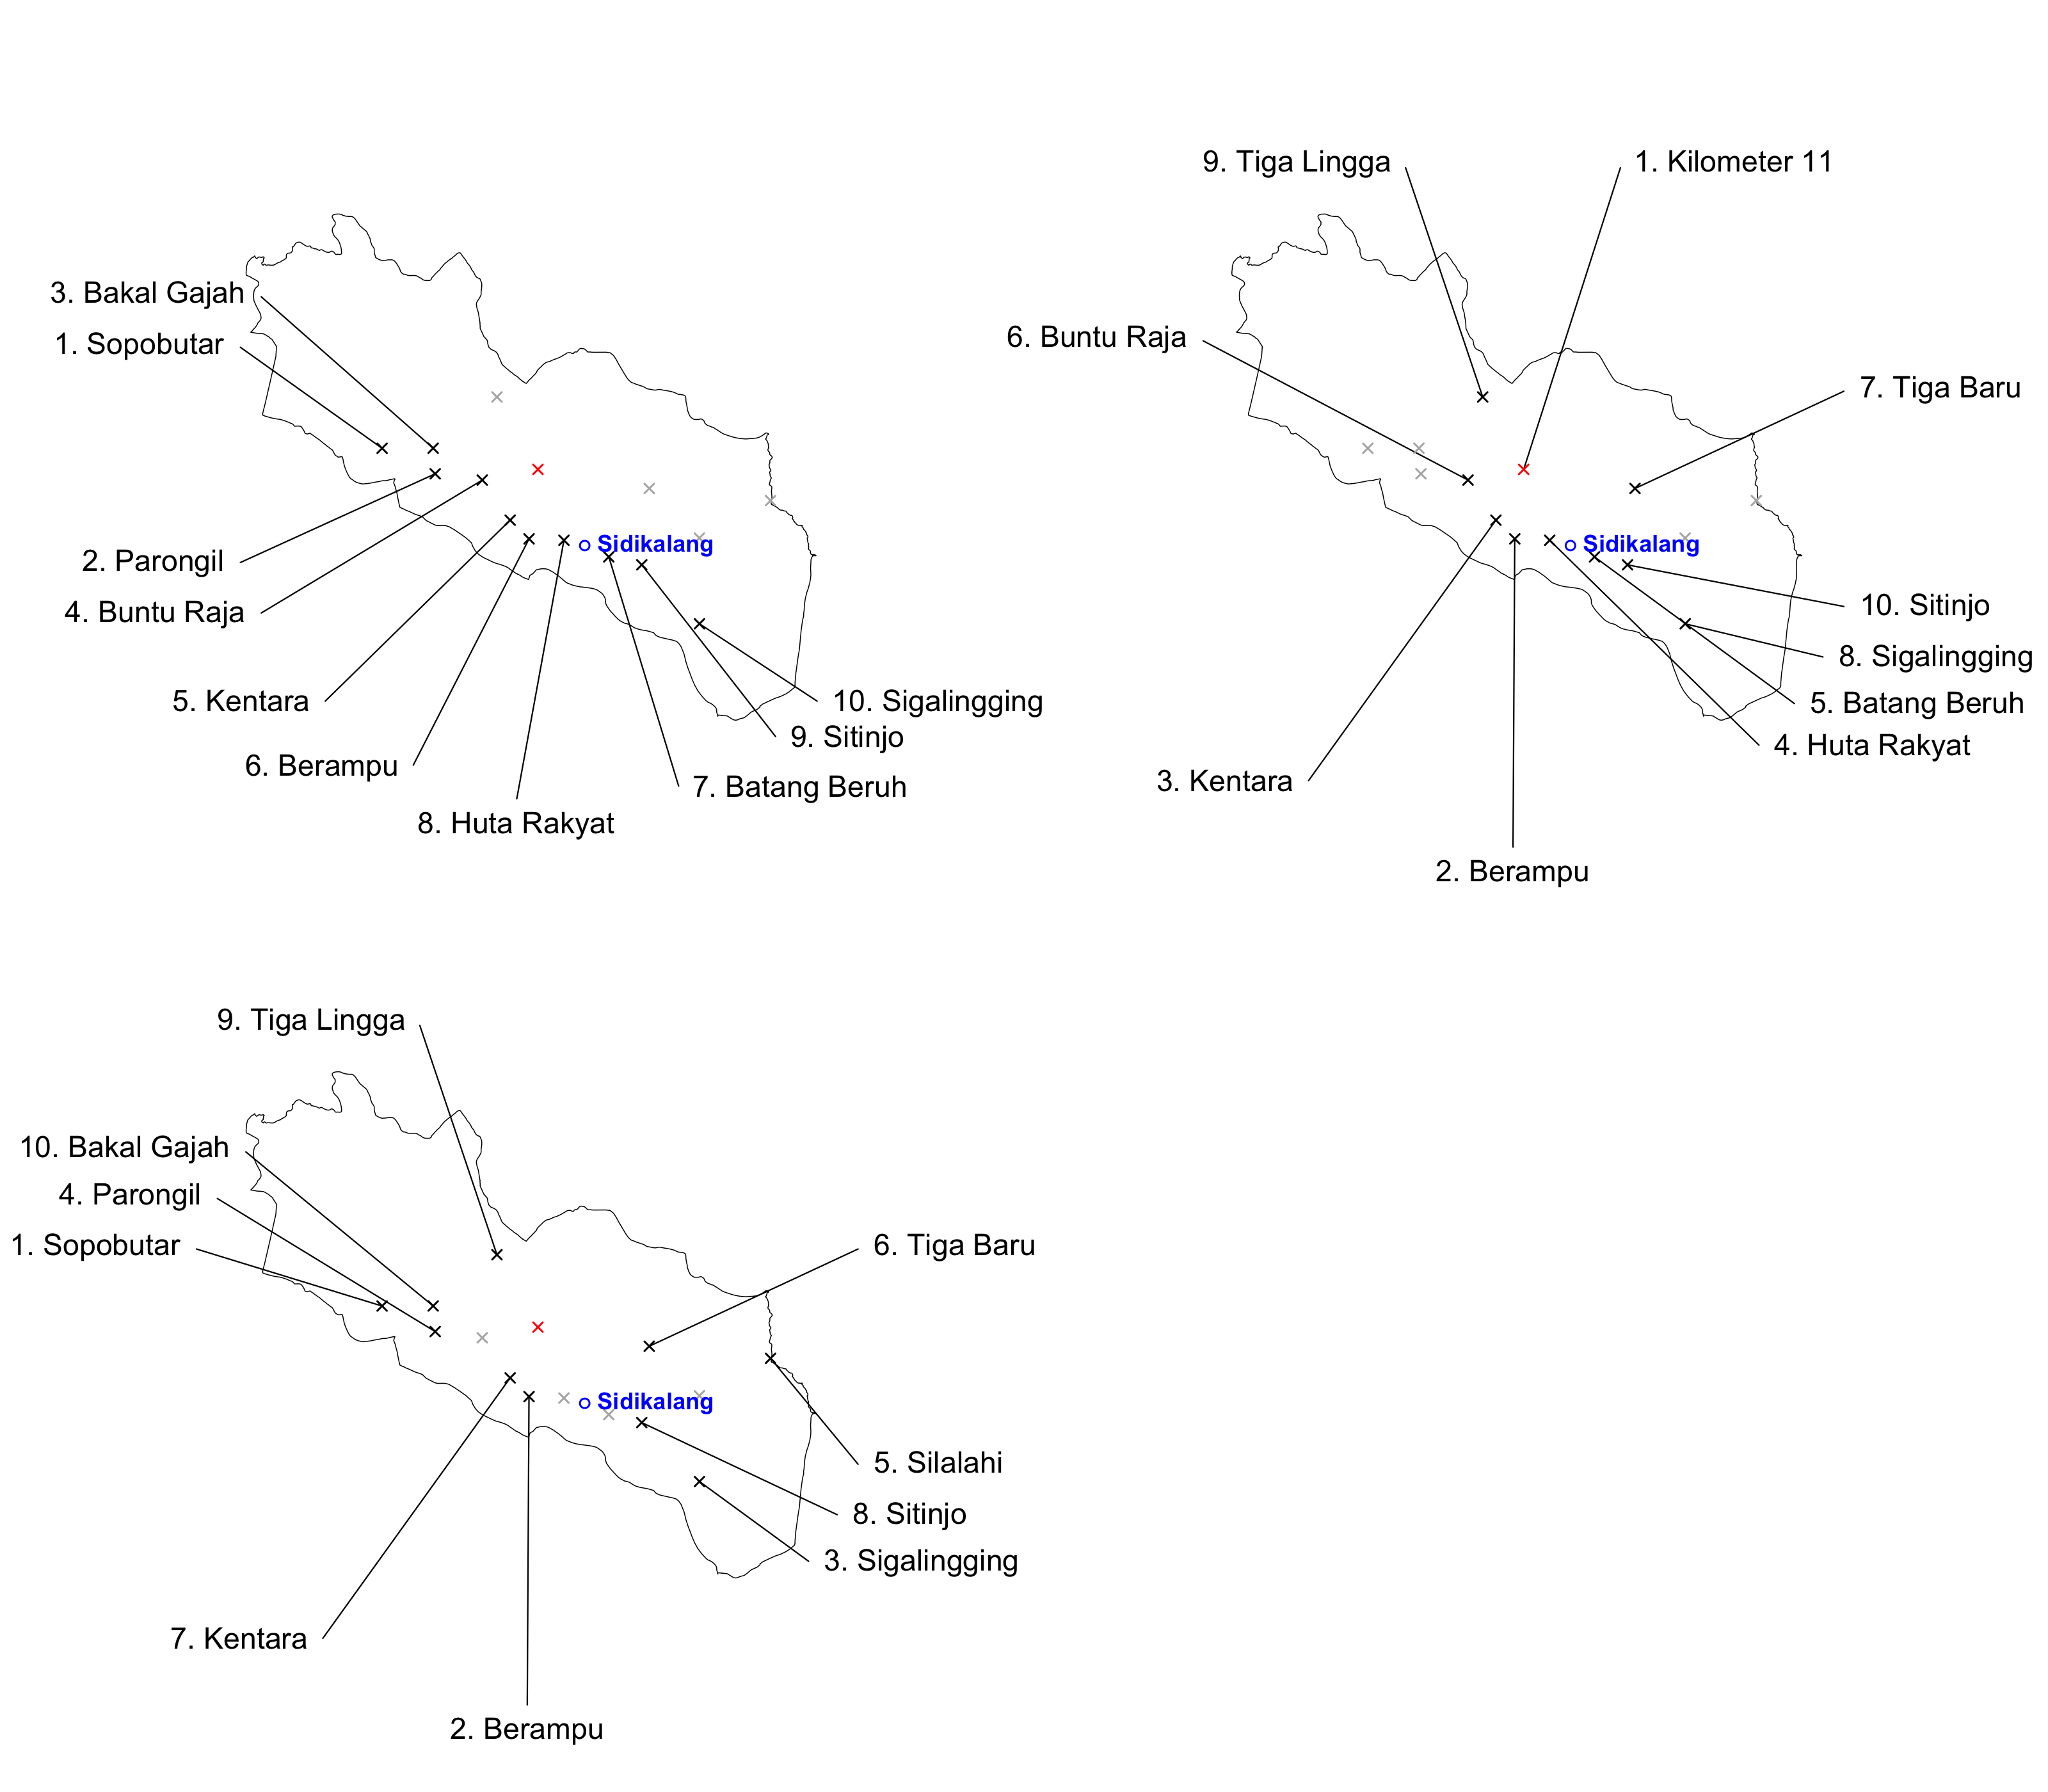
\includegraphics[width=\textwidth]{figs/dairi_all_rank_map.png}
\caption{Mapped best ranked sites in Dairi using catchment definitions of (a) distance-based 
  limits of 30 km (Table \ref{tab:dairi_dist}); (b) travel time-based limits of 100 
  minutes (Table \ref{tab:dairi_time}); and (c) tesselated catchments (Table 
  \ref{tab:dairi_stretch}). Site with ranks shaded in grey were suggested by surveillance study stakeholders. 
 Eco-constraints are indicated in green (pass) and purple (fail), summarised as ``Eco-constraints Present''.}
\label{fig:maps_dairi}
\end{figure}
\clearpage
\subsubsection{Langkat}
% latex table generated in R 4.3.1 by xtable 1.8-4 package
% Wed Sep  4 16:11:51 2024
\begin{table}[ht]
\centering
\begingroup\fontsize{8pt}{9pt}\selectfont
\begin{tabular}{C{0.03\textwidth}C{0.12\textwidth}C{0.09\textwidth}C{0.08\textwidth}C{0.08\textwidth}C{0.08\textwidth}C{0.07\textwidth}C{0.07\textwidth}C{0.07\textwidth}C{0.07\textwidth}}
 Rank & Name & Catchment Size & Objective Mean & Objective Std Dev & Eco-constraints  Present & Human Pop & Croplands & Oil Palm & Forest Loss \\ 
 {1} & Bukit Lawang & 135 & \cellcolor[HTML]{BD0026}\textcolor[HTML]{FFFFFF}{0.96} & \cellcolor[HTML]{FC4E2A}\textcolor[HTML]{000000}{0.36} & \cellcolor[HTML]{FD8D3C}\textcolor[HTML]{000000}{4} & \cellcolor[HTML]{90EE90}{******} & \cellcolor[HTML]{90EE90}{ 0.04} & \cellcolor[HTML]{90EE90}{36.83} & \cellcolor[HTML]{90EE90}{0.27} \\ 
  {2} & Stabat Lama & 130 & \cellcolor[HTML]{BD0026}\textcolor[HTML]{FFFFFF}{0.96} & \cellcolor[HTML]{FC4E2A}\textcolor[HTML]{000000}{0.33} & \cellcolor[HTML]{FD8D3C}\textcolor[HTML]{000000}{4} & \cellcolor[HTML]{90EE90}{******} & \cellcolor[HTML]{90EE90}{22.03} & \cellcolor[HTML]{90EE90}{37.00} & \cellcolor[HTML]{90EE90}{0.27} \\ 
  {3} & Bahorok & 134 & \cellcolor[HTML]{BD0026}\textcolor[HTML]{FFFFFF}{0.94} & \cellcolor[HTML]{FC4E2A}\textcolor[HTML]{000000}{0.36} & \cellcolor[HTML]{FD8D3C}\textcolor[HTML]{000000}{4} & \cellcolor[HTML]{90EE90}{******} & \cellcolor[HTML]{90EE90}{ 2.99} & \cellcolor[HTML]{90EE90}{36.83} & \cellcolor[HTML]{90EE90}{0.27} \\ 
  {4} & Tanjung Beringin & 134 & \cellcolor[HTML]{BD0026}\textcolor[HTML]{FFFFFF}{0.90} & \cellcolor[HTML]{FC4E2A}\textcolor[HTML]{000000}{0.36} & \cellcolor[HTML]{FD8D3C}\textcolor[HTML]{000000}{4} & \cellcolor[HTML]{90EE90}{******} & \cellcolor[HTML]{90EE90}{ 2.99} & \cellcolor[HTML]{90EE90}{37.00} & \cellcolor[HTML]{90EE90}{0.27} \\ 
  {5} & Tanjung Langkat & 132 & \cellcolor[HTML]{BD0026}\textcolor[HTML]{FFFFFF}{0.82} & \cellcolor[HTML]{FC4E2A}\textcolor[HTML]{000000}{0.39} & \cellcolor[HTML]{FD8D3C}\textcolor[HTML]{000000}{4} & \cellcolor[HTML]{90EE90}{******} & \cellcolor[HTML]{90EE90}{ 7.97} & \cellcolor[HTML]{90EE90}{37.00} & \cellcolor[HTML]{90EE90}{0.27} \\ 
  \cellcolor{lightgray}{6} & Ujung Bandar & 132 & \cellcolor[HTML]{E31A1C}\textcolor[HTML]{FFFFFF}{0.79} & \cellcolor[HTML]{FC4E2A}\textcolor[HTML]{000000}{0.37} & \cellcolor[HTML]{FD8D3C}\textcolor[HTML]{000000}{4} & \cellcolor[HTML]{90EE90}{******} & \cellcolor[HTML]{90EE90}{13.95} & \cellcolor[HTML]{90EE90}{37.00} & \cellcolor[HTML]{90EE90}{0.27} \\ 
  \cellcolor{lightgray}{7} & Klinik Siti & 133 & \cellcolor[HTML]{E31A1C}\textcolor[HTML]{FFFFFF}{0.77} & \cellcolor[HTML]{E31A1C}\textcolor[HTML]{FFFFFF}{0.40} & \cellcolor[HTML]{FD8D3C}\textcolor[HTML]{000000}{4} & \cellcolor[HTML]{90EE90}{******} & \cellcolor[HTML]{90EE90}{ 7.97} & \cellcolor[HTML]{90EE90}{37.00} & \cellcolor[HTML]{90EE90}{0.27} \\ 
  {8} & Marike & 131 & \cellcolor[HTML]{E31A1C}\textcolor[HTML]{FFFFFF}{0.77} & \cellcolor[HTML]{FC4E2A}\textcolor[HTML]{000000}{0.39} & \cellcolor[HTML]{FD8D3C}\textcolor[HTML]{000000}{4} & \cellcolor[HTML]{90EE90}{******} & \cellcolor[HTML]{90EE90}{13.95} & \cellcolor[HTML]{90EE90}{37.00} & \cellcolor[HTML]{90EE90}{0.27} \\ 
  {9} & Serapit & 133 & \cellcolor[HTML]{E31A1C}\textcolor[HTML]{FFFFFF}{0.70} & \cellcolor[HTML]{E31A1C}\textcolor[HTML]{FFFFFF}{0.45} & \cellcolor[HTML]{FD8D3C}\textcolor[HTML]{000000}{4} & \cellcolor[HTML]{90EE90}{******} & \cellcolor[HTML]{90EE90}{13.97} & \cellcolor[HTML]{90EE90}{37.00} & \cellcolor[HTML]{90EE90}{0.27} \\ 
  \cellcolor{lightgray}{10} & Desa Bunga Rinte & 132 & \cellcolor[HTML]{E31A1C}\textcolor[HTML]{FFFFFF}{0.69} & \cellcolor[HTML]{E31A1C}\textcolor[HTML]{FFFFFF}{0.39} & \cellcolor[HTML]{FD8D3C}\textcolor[HTML]{000000}{4} & \cellcolor[HTML]{90EE90}{******} & \cellcolor[HTML]{90EE90}{17.96} & \cellcolor[HTML]{90EE90}{37.00} & \cellcolor[HTML]{90EE90}{0.27} \\ 
  {-} & Sei Bambam & 130 & \cellcolor[HTML]{FC4E2A}\textcolor[HTML]{000000}{0.65} & \cellcolor[HTML]{E31A1C}\textcolor[HTML]{FFFFFF}{0.46} & \cellcolor[HTML]{FD8D3C}\textcolor[HTML]{000000}{4} & \cellcolor[HTML]{90EE90}{******} & \cellcolor[HTML]{90EE90}{42.87} & \cellcolor[HTML]{90EE90}{37.00} & \cellcolor[HTML]{90EE90}{0.23} \\ 
  {-} & Besitang & 117 & \cellcolor[HTML]{FC4E2A}\textcolor[HTML]{000000}{0.64} & \cellcolor[HTML]{BD0026}\textcolor[HTML]{FFFFFF}{0.53} & \cellcolor[HTML]{FD8D3C}\textcolor[HTML]{000000}{4} & \cellcolor[HTML]{90EE90}{******} & \cellcolor[HTML]{90EE90}{64.91} & \cellcolor[HTML]{90EE90}{37.00} & \cellcolor[HTML]{90EE90}{0.35} \\ 
  {-} & Kuala & 131 & \cellcolor[HTML]{FC4E2A}\textcolor[HTML]{000000}{0.63} & \cellcolor[HTML]{E31A1C}\textcolor[HTML]{FFFFFF}{0.44} & \cellcolor[HTML]{FD8D3C}\textcolor[HTML]{000000}{4} & \cellcolor[HTML]{90EE90}{*******} & \cellcolor[HTML]{90EE90}{24.92} & \cellcolor[HTML]{90EE90}{37.00} & \cellcolor[HTML]{90EE90}{0.27} \\ 
  {-} & Sawit Seberang & 130 & \cellcolor[HTML]{FD8D3C}\textcolor[HTML]{000000}{0.51} & \cellcolor[HTML]{E31A1C}\textcolor[HTML]{FFFFFF}{0.45} & \cellcolor[HTML]{FD8D3C}\textcolor[HTML]{000000}{4} & \cellcolor[HTML]{90EE90}{******} & \cellcolor[HTML]{90EE90}{64.91} & \cellcolor[HTML]{90EE90}{37.00} & \cellcolor[HTML]{90EE90}{0.23} \\ 
  {-} & Namu Ukur & 132 & \cellcolor[HTML]{FD8D3C}\textcolor[HTML]{000000}{0.50} & \cellcolor[HTML]{E31A1C}\textcolor[HTML]{FFFFFF}{0.43} & \cellcolor[HTML]{FD8D3C}\textcolor[HTML]{000000}{4} & \cellcolor[HTML]{90EE90}{*******} & \cellcolor[HTML]{90EE90}{24.92} & \cellcolor[HTML]{90EE90}{37.00} & \cellcolor[HTML]{90EE90}{0.27} \\ 
  {-} & Tangkahan Durian & 112 & \cellcolor[HTML]{FD8D3C}\textcolor[HTML]{000000}{0.48} & \cellcolor[HTML]{E31A1C}\textcolor[HTML]{FFFFFF}{0.42} & \cellcolor[HTML]{FD8D3C}\textcolor[HTML]{000000}{4} & \cellcolor[HTML]{90EE90}{******} & \cellcolor[HTML]{90EE90}{64.91} & \cellcolor[HTML]{90EE90}{37.00} & \cellcolor[HTML]{90EE90}{0.35} \\ 
  {-} & Namu Trasi & 130 & \cellcolor[HTML]{FD8D3C}\textcolor[HTML]{000000}{0.45} & \cellcolor[HTML]{E31A1C}\textcolor[HTML]{FFFFFF}{0.41} & \cellcolor[HTML]{FD8D3C}\textcolor[HTML]{000000}{4} & \cellcolor[HTML]{90EE90}{*******} & \cellcolor[HTML]{90EE90}{24.92} & \cellcolor[HTML]{90EE90}{37.00} & \cellcolor[HTML]{90EE90}{0.27} \\ 
  {-} & Selesei & 134 & \cellcolor[HTML]{FD8D3C}\textcolor[HTML]{000000}{0.44} & \cellcolor[HTML]{E31A1C}\textcolor[HTML]{FFFFFF}{0.41} & \cellcolor[HTML]{FD8D3C}\textcolor[HTML]{000000}{4} & \cellcolor[HTML]{90EE90}{*******} & \cellcolor[HTML]{90EE90}{24.92} & \cellcolor[HTML]{90EE90}{37.00} & \cellcolor[HTML]{90EE90}{0.27} \\ 
  {-} & Pangkalan Susu &  98 & \cellcolor[HTML]{FEB24C}\textcolor[HTML]{000000}{0.40} & \cellcolor[HTML]{FC4E2A}\textcolor[HTML]{000000}{0.33} & \cellcolor[HTML]{FD8D3C}\textcolor[HTML]{000000}{4} & \cellcolor[HTML]{90EE90}{******} & \cellcolor[HTML]{90EE90}{64.91} & \cellcolor[HTML]{90EE90}{37.00} & \cellcolor[HTML]{90EE90}{0.35} \\ 
  {-} & Tanjung Selamat & 123 & \cellcolor[HTML]{FEB24C}\textcolor[HTML]{000000}{0.38} & \cellcolor[HTML]{FC4E2A}\textcolor[HTML]{000000}{0.39} & \cellcolor[HTML]{FD8D3C}\textcolor[HTML]{000000}{4} & \cellcolor[HTML]{90EE90}{******} & \cellcolor[HTML]{90EE90}{64.91} & \cellcolor[HTML]{90EE90}{37.00} & \cellcolor[HTML]{90EE90}{0.23} \\ 
  {-} & Pangkalan Brandan &  98 & \cellcolor[HTML]{FEB24C}\textcolor[HTML]{000000}{0.37} & \cellcolor[HTML]{FC4E2A}\textcolor[HTML]{000000}{0.34} & \cellcolor[HTML]{FD8D3C}\textcolor[HTML]{000000}{4} & \cellcolor[HTML]{90EE90}{******} & \cellcolor[HTML]{90EE90}{64.91} & \cellcolor[HTML]{90EE90}{37.00} & \cellcolor[HTML]{90EE90}{0.35} \\ 
  {-} & Desa Lama &  93 & \cellcolor[HTML]{FEB24C}\textcolor[HTML]{000000}{0.31} & \cellcolor[HTML]{FD8D3C}\textcolor[HTML]{000000}{0.26} & \cellcolor[HTML]{FD8D3C}\textcolor[HTML]{000000}{4} & \cellcolor[HTML]{90EE90}{******} & \cellcolor[HTML]{90EE90}{66.90} & \cellcolor[HTML]{90EE90}{37.00} & \cellcolor[HTML]{90EE90}{0.16} \\ 
  {-} & Sambi Rejo & 126 & \cellcolor[HTML]{FEB24C}\textcolor[HTML]{000000}{0.28} & \cellcolor[HTML]{FD8D3C}\textcolor[HTML]{000000}{0.31} & \cellcolor[HTML]{FD8D3C}\textcolor[HTML]{000000}{4} & \cellcolor[HTML]{90EE90}{*******} & \cellcolor[HTML]{90EE90}{28.93} & \cellcolor[HTML]{90EE90}{37.00} & \cellcolor[HTML]{90EE90}{0.27} \\ 
  {-} & Securai &  81 & \cellcolor[HTML]{FEB24C}\textcolor[HTML]{000000}{0.27} & \cellcolor[HTML]{FD8D3C}\textcolor[HTML]{000000}{0.27} & \cellcolor[HTML]{FD8D3C}\textcolor[HTML]{000000}{4} & \cellcolor[HTML]{90EE90}{******} & \cellcolor[HTML]{90EE90}{64.91} & \cellcolor[HTML]{90EE90}{37.00} & \cellcolor[HTML]{90EE90}{0.23} \\ 
  {-} & Gebang & 103 & \cellcolor[HTML]{FED976}\textcolor[HTML]{000000}{0.24} & \cellcolor[HTML]{FD8D3C}\textcolor[HTML]{000000}{0.26} & \cellcolor[HTML]{FD8D3C}\textcolor[HTML]{000000}{4} & \cellcolor[HTML]{90EE90}{******} & \cellcolor[HTML]{90EE90}{64.91} & \cellcolor[HTML]{90EE90}{37.00} & \cellcolor[HTML]{90EE90}{0.23} \\ 
  {-} & Stabat & 123 & \cellcolor[HTML]{FED976}\textcolor[HTML]{000000}{0.24} & \cellcolor[HTML]{FD8D3C}\textcolor[HTML]{000000}{0.27} & \cellcolor[HTML]{FD8D3C}\textcolor[HTML]{000000}{4} & \cellcolor[HTML]{90EE90}{*******} & \cellcolor[HTML]{90EE90}{42.87} & \cellcolor[HTML]{90EE90}{37.00} & \cellcolor[HTML]{90EE90}{0.27} \\ 
  {-} & Karang Rejo & 120 & \cellcolor[HTML]{FED976}\textcolor[HTML]{000000}{0.19} & \cellcolor[HTML]{FEB24C}\textcolor[HTML]{000000}{0.20} & \cellcolor[HTML]{FD8D3C}\textcolor[HTML]{000000}{4} & \cellcolor[HTML]{90EE90}{*******} & \cellcolor[HTML]{90EE90}{69.79} & \cellcolor[HTML]{90EE90}{37.00} & \cellcolor[HTML]{90EE90}{0.27} \\ 
  {-} & Hinai Kiri & 107 & \cellcolor[HTML]{FED976}\textcolor[HTML]{000000}{0.18} & \cellcolor[HTML]{FEB24C}\textcolor[HTML]{000000}{0.21} & \cellcolor[HTML]{FD8D3C}\textcolor[HTML]{000000}{4} & \cellcolor[HTML]{90EE90}{*******} & \cellcolor[HTML]{90EE90}{64.91} & \cellcolor[HTML]{90EE90}{37.00} & \cellcolor[HTML]{90EE90}{0.23} \\ 
  {-} & Pantai Cermin &  88 & \cellcolor[HTML]{FED976}\textcolor[HTML]{000000}{0.18} & \cellcolor[HTML]{FEB24C}\textcolor[HTML]{000000}{0.21} & \cellcolor[HTML]{FD8D3C}\textcolor[HTML]{000000}{4} & \cellcolor[HTML]{90EE90}{******} & \cellcolor[HTML]{90EE90}{64.91} & \cellcolor[HTML]{90EE90}{37.00} & \cellcolor[HTML]{90EE90}{0.23} \\ 
  {-} & Desa Teluk & 109 & \cellcolor[HTML]{FED976}\textcolor[HTML]{000000}{0.14} & \cellcolor[HTML]{FED976}\textcolor[HTML]{000000}{0.14} & \cellcolor[HTML]{FD8D3C}\textcolor[HTML]{000000}{4} & \cellcolor[HTML]{90EE90}{*******} & \cellcolor[HTML]{90EE90}{69.79} & \cellcolor[HTML]{90EE90}{37.00} & \cellcolor[HTML]{90EE90}{0.23} \\ 
  {-} & Secanggang &  92 & \cellcolor[HTML]{FED976}\textcolor[HTML]{000000}{0.12} & \cellcolor[HTML]{FED976}\textcolor[HTML]{000000}{0.12} & \cellcolor[HTML]{FD8D3C}\textcolor[HTML]{000000}{4} & \cellcolor[HTML]{90EE90}{*******} & \cellcolor[HTML]{90EE90}{69.79} & \cellcolor[HTML]{90EE90}{37.00} & \cellcolor[HTML]{90EE90}{0.23} \\ 
  \end{tabular}
\endgroup
\caption{Langkat sites (distance catchments, 30 km)} 
\label{tab:langkat_dist}
\end{table}
% latex table generated in R 4.3.1 by xtable 1.8-4 package
% Wed Sep  4 16:11:51 2024
\begin{table}[ht]
\centering
\begingroup\fontsize{8pt}{9pt}\selectfont
\begin{tabular}{C{0.03\textwidth}C{0.12\textwidth}C{0.09\textwidth}C{0.08\textwidth}C{0.08\textwidth}C{0.08\textwidth}C{0.07\textwidth}C{0.07\textwidth}C{0.07\textwidth}C{0.07\textwidth}}
 Rank & Name & Catchment Size & Objective Mean & Objective Std Dev & Eco-constraints  Present & Human Pop & Croplands & Oil Palm & Forest Loss \\ 
 \cellcolor{lightgray}{1} & Ujung Bandar &  32 & \cellcolor[HTML]{BD0026}\textcolor[HTML]{FFFFFF}{0.79} & \cellcolor[HTML]{FD8D3C}\textcolor[HTML]{000000}{0.31} & \cellcolor[HTML]{FED976}\textcolor[HTML]{000000}{3} & \cellcolor[HTML]{90EE90}{*****} & \cellcolor[HTML]{9370D8}{ 0.00} & \cellcolor[HTML]{90EE90}{36.93} & \cellcolor[HTML]{90EE90}{0.27} \\ 
  {2} & Bukit Lawang &  81 & \cellcolor[HTML]{BD0026}\textcolor[HTML]{FFFFFF}{0.70} & \cellcolor[HTML]{E31A1C}\textcolor[HTML]{FFFFFF}{0.36} & \cellcolor[HTML]{FED976}\textcolor[HTML]{000000}{3} & \cellcolor[HTML]{90EE90}{******} & \cellcolor[HTML]{9370D8}{ 0.00} & \cellcolor[HTML]{90EE90}{37.00} & \cellcolor[HTML]{90EE90}{0.27} \\ 
  {3} & Stabat Lama &  83 & \cellcolor[HTML]{E31A1C}\textcolor[HTML]{FFFFFF}{0.67} & \cellcolor[HTML]{BD0026}\textcolor[HTML]{FFFFFF}{0.40} & \cellcolor[HTML]{BD0026}\textcolor[HTML]{FFFFFF}{4} & \cellcolor[HTML]{90EE90}{******} & \cellcolor[HTML]{90EE90}{13.97} & \cellcolor[HTML]{90EE90}{37.00} & \cellcolor[HTML]{90EE90}{0.27} \\ 
  \cellcolor{lightgray}{4} & Desa Bunga Rinte &  56 & \cellcolor[HTML]{E31A1C}\textcolor[HTML]{FFFFFF}{0.61} & \cellcolor[HTML]{BD0026}\textcolor[HTML]{FFFFFF}{0.42} & \cellcolor[HTML]{BD0026}\textcolor[HTML]{FFFFFF}{4} & \cellcolor[HTML]{90EE90}{******} & \cellcolor[HTML]{90EE90}{24.92} & \cellcolor[HTML]{90EE90}{37.00} & \cellcolor[HTML]{90EE90}{0.27} \\ 
  {5} & Marike &  66 & \cellcolor[HTML]{FC4E2A}\textcolor[HTML]{000000}{0.59} & \cellcolor[HTML]{BD0026}\textcolor[HTML]{FFFFFF}{0.40} & \cellcolor[HTML]{BD0026}\textcolor[HTML]{FFFFFF}{4} & \cellcolor[HTML]{90EE90}{******} & \cellcolor[HTML]{90EE90}{15.96} & \cellcolor[HTML]{90EE90}{37.00} & \cellcolor[HTML]{90EE90}{0.27} \\ 
  {6} & Bahorok & 118 & \cellcolor[HTML]{FC4E2A}\textcolor[HTML]{000000}{0.52} & \cellcolor[HTML]{BD0026}\textcolor[HTML]{FFFFFF}{0.42} & \cellcolor[HTML]{BD0026}\textcolor[HTML]{FFFFFF}{4} & \cellcolor[HTML]{90EE90}{*******} & \cellcolor[HTML]{90EE90}{24.92} & \cellcolor[HTML]{90EE90}{37.00} & \cellcolor[HTML]{90EE90}{0.27} \\ 
  {7} & Tanjung Beringin & 156 & \cellcolor[HTML]{FD8D3C}\textcolor[HTML]{000000}{0.42} & \cellcolor[HTML]{BD0026}\textcolor[HTML]{FFFFFF}{0.41} & \cellcolor[HTML]{BD0026}\textcolor[HTML]{FFFFFF}{4} & \cellcolor[HTML]{90EE90}{*******} & \cellcolor[HTML]{90EE90}{67.95} & \cellcolor[HTML]{90EE90}{37.00} & \cellcolor[HTML]{90EE90}{0.27} \\ 
  {8} & Serapit & 220 & \cellcolor[HTML]{FEB24C}\textcolor[HTML]{000000}{0.39} & \cellcolor[HTML]{BD0026}\textcolor[HTML]{FFFFFF}{0.40} & \cellcolor[HTML]{BD0026}\textcolor[HTML]{FFFFFF}{4} & \cellcolor[HTML]{90EE90}{*******} & \cellcolor[HTML]{90EE90}{94.86} & \cellcolor[HTML]{90EE90}{37.00} & \cellcolor[HTML]{90EE90}{0.27} \\ 
  {9} & Tanjung Langkat & 237 & \cellcolor[HTML]{FEB24C}\textcolor[HTML]{000000}{0.37} & \cellcolor[HTML]{BD0026}\textcolor[HTML]{FFFFFF}{0.40} & \cellcolor[HTML]{BD0026}\textcolor[HTML]{FFFFFF}{4} & \cellcolor[HTML]{90EE90}{*******} & \cellcolor[HTML]{90EE90}{94.86} & \cellcolor[HTML]{90EE90}{37.00} & \cellcolor[HTML]{90EE90}{0.27} \\ 
  {10} & Sei Bambam & 199 & \cellcolor[HTML]{FEB24C}\textcolor[HTML]{000000}{0.35} & \cellcolor[HTML]{E31A1C}\textcolor[HTML]{FFFFFF}{0.38} & \cellcolor[HTML]{BD0026}\textcolor[HTML]{FFFFFF}{4} & \cellcolor[HTML]{90EE90}{*******} & \cellcolor[HTML]{90EE90}{67.95} & \cellcolor[HTML]{90EE90}{37.00} & \cellcolor[HTML]{90EE90}{0.27} \\ 
  \cellcolor{lightgray}{-} & Klinik Siti & 260 & \cellcolor[HTML]{FEB24C}\textcolor[HTML]{000000}{0.35} & \cellcolor[HTML]{E31A1C}\textcolor[HTML]{FFFFFF}{0.37} & \cellcolor[HTML]{BD0026}\textcolor[HTML]{FFFFFF}{4} & \cellcolor[HTML]{90EE90}{*******} & \cellcolor[HTML]{90EE90}{98.95} & \cellcolor[HTML]{90EE90}{37.00} & \cellcolor[HTML]{90EE90}{0.27} \\ 
  {-} & Kuala & 224 & \cellcolor[HTML]{FEB24C}\textcolor[HTML]{000000}{0.34} & \cellcolor[HTML]{E31A1C}\textcolor[HTML]{FFFFFF}{0.38} & \cellcolor[HTML]{BD0026}\textcolor[HTML]{FFFFFF}{4} & \cellcolor[HTML]{90EE90}{*******} & \cellcolor[HTML]{90EE90}{94.86} & \cellcolor[HTML]{90EE90}{37.00} & \cellcolor[HTML]{90EE90}{0.27} \\ 
  {-} & Namu Ukur & 389 & \cellcolor[HTML]{FED976}\textcolor[HTML]{000000}{0.32} & \cellcolor[HTML]{FC4E2A}\textcolor[HTML]{000000}{0.33} & \cellcolor[HTML]{BD0026}\textcolor[HTML]{FFFFFF}{4} & \cellcolor[HTML]{90EE90}{*******} & \cellcolor[HTML]{90EE90}{98.95} & \cellcolor[HTML]{90EE90}{37.00} & \cellcolor[HTML]{90EE90}{0.27} \\ 
  {-} & Selesei & 419 & \cellcolor[HTML]{FED976}\textcolor[HTML]{000000}{0.32} & \cellcolor[HTML]{FC4E2A}\textcolor[HTML]{000000}{0.32} & \cellcolor[HTML]{BD0026}\textcolor[HTML]{FFFFFF}{4} & \cellcolor[HTML]{90EE90}{*******} & \cellcolor[HTML]{90EE90}{98.95} & \cellcolor[HTML]{90EE90}{37.00} & \cellcolor[HTML]{90EE90}{0.27} \\ 
  {-} & Namu Trasi & 445 & \cellcolor[HTML]{FED976}\textcolor[HTML]{000000}{0.31} & \cellcolor[HTML]{FD8D3C}\textcolor[HTML]{000000}{0.31} & \cellcolor[HTML]{BD0026}\textcolor[HTML]{FFFFFF}{4} & \cellcolor[HTML]{90EE90}{*******} & \cellcolor[HTML]{90EE90}{98.95} & \cellcolor[HTML]{90EE90}{37.00} & \cellcolor[HTML]{90EE90}{0.27} \\ 
  {-} & Stabat & 525 & \cellcolor[HTML]{FED976}\textcolor[HTML]{000000}{0.31} & \cellcolor[HTML]{FD8D3C}\textcolor[HTML]{000000}{0.30} & \cellcolor[HTML]{BD0026}\textcolor[HTML]{FFFFFF}{4} & \cellcolor[HTML]{90EE90}{*******} & \cellcolor[HTML]{90EE90}{98.95} & \cellcolor[HTML]{90EE90}{37.00} & \cellcolor[HTML]{90EE90}{0.27} \\ 
  {-} & Sambi Rejo & 479 & \cellcolor[HTML]{FED976}\textcolor[HTML]{000000}{0.31} & \cellcolor[HTML]{FD8D3C}\textcolor[HTML]{000000}{0.30} & \cellcolor[HTML]{BD0026}\textcolor[HTML]{FFFFFF}{4} & \cellcolor[HTML]{90EE90}{*******} & \cellcolor[HTML]{90EE90}{98.95} & \cellcolor[HTML]{90EE90}{37.00} & \cellcolor[HTML]{90EE90}{0.27} \\ 
  {-} & Karang Rejo & 522 & \cellcolor[HTML]{FED976}\textcolor[HTML]{000000}{0.30} & \cellcolor[HTML]{FD8D3C}\textcolor[HTML]{000000}{0.30} & \cellcolor[HTML]{BD0026}\textcolor[HTML]{FFFFFF}{4} & \cellcolor[HTML]{90EE90}{*******} & \cellcolor[HTML]{90EE90}{98.95} & \cellcolor[HTML]{90EE90}{37.00} & \cellcolor[HTML]{90EE90}{0.27} \\ 
  {-} & Sawit Seberang & 249 & \cellcolor[HTML]{FED976}\textcolor[HTML]{000000}{0.30} & \cellcolor[HTML]{FC4E2A}\textcolor[HTML]{000000}{0.32} & \cellcolor[HTML]{BD0026}\textcolor[HTML]{FFFFFF}{4} & \cellcolor[HTML]{90EE90}{*******} & \cellcolor[HTML]{90EE90}{94.86} & \cellcolor[HTML]{90EE90}{37.00} & \cellcolor[HTML]{90EE90}{0.27} \\ 
  {-} & Gebang & 468 & \cellcolor[HTML]{FED976}\textcolor[HTML]{000000}{0.30} & \cellcolor[HTML]{FD8D3C}\textcolor[HTML]{000000}{0.29} & \cellcolor[HTML]{BD0026}\textcolor[HTML]{FFFFFF}{4} & \cellcolor[HTML]{90EE90}{*******} & \cellcolor[HTML]{90EE90}{98.95} & \cellcolor[HTML]{90EE90}{37.00} & \cellcolor[HTML]{90EE90}{0.27} \\ 
  {-} & Pangkalan Brandan & 418 & \cellcolor[HTML]{FED976}\textcolor[HTML]{000000}{0.29} & \cellcolor[HTML]{FD8D3C}\textcolor[HTML]{000000}{0.31} & \cellcolor[HTML]{BD0026}\textcolor[HTML]{FFFFFF}{4} & \cellcolor[HTML]{90EE90}{*******} & \cellcolor[HTML]{90EE90}{98.95} & \cellcolor[HTML]{90EE90}{37.00} & \cellcolor[HTML]{90EE90}{0.27} \\ 
  {-} & Tangkahan Durian & 405 & \cellcolor[HTML]{FED976}\textcolor[HTML]{000000}{0.29} & \cellcolor[HTML]{FD8D3C}\textcolor[HTML]{000000}{0.31} & \cellcolor[HTML]{BD0026}\textcolor[HTML]{FFFFFF}{4} & \cellcolor[HTML]{90EE90}{*******} & \cellcolor[HTML]{90EE90}{98.95} & \cellcolor[HTML]{90EE90}{37.00} & \cellcolor[HTML]{90EE90}{0.27} \\ 
  {-} & Tanjung Selamat & 324 & \cellcolor[HTML]{FED976}\textcolor[HTML]{000000}{0.29} & \cellcolor[HTML]{FD8D3C}\textcolor[HTML]{000000}{0.31} & \cellcolor[HTML]{BD0026}\textcolor[HTML]{FFFFFF}{4} & \cellcolor[HTML]{90EE90}{*******} & \cellcolor[HTML]{90EE90}{98.95} & \cellcolor[HTML]{90EE90}{37.00} & \cellcolor[HTML]{90EE90}{0.27} \\ 
  {-} & Besitang & 381 & \cellcolor[HTML]{FED976}\textcolor[HTML]{000000}{0.28} & \cellcolor[HTML]{FD8D3C}\textcolor[HTML]{000000}{0.31} & \cellcolor[HTML]{BD0026}\textcolor[HTML]{FFFFFF}{4} & \cellcolor[HTML]{90EE90}{*******} & \cellcolor[HTML]{90EE90}{98.95} & \cellcolor[HTML]{90EE90}{37.00} & \cellcolor[HTML]{90EE90}{0.27} \\ 
  {-} & Hinai Kiri & 371 & \cellcolor[HTML]{FED976}\textcolor[HTML]{000000}{0.26} & \cellcolor[HTML]{FEB24C}\textcolor[HTML]{000000}{0.27} & \cellcolor[HTML]{BD0026}\textcolor[HTML]{FFFFFF}{4} & \cellcolor[HTML]{90EE90}{*******} & \cellcolor[HTML]{90EE90}{98.95} & \cellcolor[HTML]{90EE90}{37.00} & \cellcolor[HTML]{90EE90}{0.27} \\ 
  {-} & Pantai Cermin & 349 & \cellcolor[HTML]{FED976}\textcolor[HTML]{000000}{0.25} & \cellcolor[HTML]{FEB24C}\textcolor[HTML]{000000}{0.26} & \cellcolor[HTML]{BD0026}\textcolor[HTML]{FFFFFF}{4} & \cellcolor[HTML]{90EE90}{*******} & \cellcolor[HTML]{90EE90}{98.95} & \cellcolor[HTML]{90EE90}{37.00} & \cellcolor[HTML]{90EE90}{0.27} \\ 
  {-} & Securai & 336 & \cellcolor[HTML]{FED976}\textcolor[HTML]{000000}{0.25} & \cellcolor[HTML]{FEB24C}\textcolor[HTML]{000000}{0.25} & \cellcolor[HTML]{BD0026}\textcolor[HTML]{FFFFFF}{4} & \cellcolor[HTML]{90EE90}{*******} & \cellcolor[HTML]{90EE90}{98.95} & \cellcolor[HTML]{90EE90}{37.00} & \cellcolor[HTML]{90EE90}{0.27} \\ 
  {-} & Desa Teluk & 323 & \cellcolor[HTML]{FED976}\textcolor[HTML]{000000}{0.24} & \cellcolor[HTML]{FEB24C}\textcolor[HTML]{000000}{0.24} & \cellcolor[HTML]{BD0026}\textcolor[HTML]{FFFFFF}{4} & \cellcolor[HTML]{90EE90}{*******} & \cellcolor[HTML]{90EE90}{98.95} & \cellcolor[HTML]{90EE90}{37.00} & \cellcolor[HTML]{90EE90}{0.27} \\ 
  {-} & Desa Lama &  96 & \cellcolor[HTML]{FED976}\textcolor[HTML]{000000}{0.23} & \cellcolor[HTML]{FED976}\textcolor[HTML]{000000}{0.20} & \cellcolor[HTML]{BD0026}\textcolor[HTML]{FFFFFF}{4} & \cellcolor[HTML]{90EE90}{******} & \cellcolor[HTML]{90EE90}{66.90} & \cellcolor[HTML]{90EE90}{37.00} & \cellcolor[HTML]{90EE90}{0.16} \\ 
  {-} & Pangkalan Susu & 232 & \cellcolor[HTML]{FED976}\textcolor[HTML]{000000}{0.23} & \cellcolor[HTML]{FED976}\textcolor[HTML]{000000}{0.23} & \cellcolor[HTML]{BD0026}\textcolor[HTML]{FFFFFF}{4} & \cellcolor[HTML]{90EE90}{*******} & \cellcolor[HTML]{90EE90}{66.90} & \cellcolor[HTML]{90EE90}{37.00} & \cellcolor[HTML]{90EE90}{0.23} \\ 
  {-} & Secanggang & 286 & \cellcolor[HTML]{FED976}\textcolor[HTML]{000000}{0.23} & \cellcolor[HTML]{FED976}\textcolor[HTML]{000000}{0.23} & \cellcolor[HTML]{BD0026}\textcolor[HTML]{FFFFFF}{4} & \cellcolor[HTML]{90EE90}{*******} & \cellcolor[HTML]{90EE90}{98.95} & \cellcolor[HTML]{90EE90}{37.00} & \cellcolor[HTML]{90EE90}{0.27} \\ 
  \end{tabular}
\endgroup
\caption{Langkat sites (travel time catchments, 100 minutes)} 
\label{tab:langkat_time}
\end{table}
% latex table generated in R 4.3.1 by xtable 1.8-4 package
% Wed Sep  4 16:11:51 2024
\begin{table}[ht]
\centering
\begingroup\fontsize{8pt}{9pt}\selectfont
\begin{tabular}{C{0.03\textwidth}C{0.12\textwidth}C{0.09\textwidth}C{0.08\textwidth}C{0.08\textwidth}C{0.08\textwidth}C{0.07\textwidth}C{0.07\textwidth}C{0.07\textwidth}C{0.07\textwidth}}
 Rank & Name & Catchment Size & Objective Mean & Objective Std Dev & Eco-constraints  Present & Human Pop & Croplands & Oil Palm & Forest Loss \\ 
 \cellcolor{lightgray}{1} & Ujung Bandar &  11 & \cellcolor[HTML]{BD0026}\textcolor[HTML]{FFFFFF}{1.17} & \cellcolor[HTML]{FC4E2A}\textcolor[HTML]{000000}{0.31} & \cellcolor[HTML]{BD0026}\textcolor[HTML]{FFFFFF}{4} & \cellcolor[HTML]{90EE90}{*****} & \cellcolor[HTML]{90EE90}{ 0.00} & \cellcolor[HTML]{90EE90}{33.93} & \cellcolor[HTML]{90EE90}{0.04} \\ 
  {2} & Bukit Lawang &  47 & \cellcolor[HTML]{BD0026}\textcolor[HTML]{FFFFFF}{1.11} & \cellcolor[HTML]{FC4E2A}\textcolor[HTML]{000000}{0.31} & \cellcolor[HTML]{FD8D3C}\textcolor[HTML]{000000}{3} & \cellcolor[HTML]{90EE90}{*****} & \cellcolor[HTML]{9370D8}{ 0.00} & \cellcolor[HTML]{90EE90}{36.83} & \cellcolor[HTML]{90EE90}{0.13} \\ 
  {3} & Stabat Lama &  28 & \cellcolor[HTML]{BD0026}\textcolor[HTML]{FFFFFF}{1.10} & \cellcolor[HTML]{FD8D3C}\textcolor[HTML]{000000}{0.22} & \cellcolor[HTML]{BD0026}\textcolor[HTML]{FFFFFF}{4} & \cellcolor[HTML]{90EE90}{*****} & \cellcolor[HTML]{90EE90}{ 0.04} & \cellcolor[HTML]{90EE90}{34.73} & \cellcolor[HTML]{90EE90}{0.05} \\ 
  \cellcolor{lightgray}{4} & Desa Bunga Rinte &  17 & \cellcolor[HTML]{BD0026}\textcolor[HTML]{FFFFFF}{1.05} & \cellcolor[HTML]{FC4E2A}\textcolor[HTML]{000000}{0.25} & \cellcolor[HTML]{FD8D3C}\textcolor[HTML]{000000}{3} & \cellcolor[HTML]{90EE90}{*****} & \cellcolor[HTML]{9370D8}{ 0.00} & \cellcolor[HTML]{90EE90}{34.08} & \cellcolor[HTML]{90EE90}{0.05} \\ 
  {5} & Marike &   3 & \cellcolor[HTML]{BD0026}\textcolor[HTML]{FFFFFF}{1.00} & \cellcolor[HTML]{FD8D3C}\textcolor[HTML]{000000}{0.19} & \cellcolor[HTML]{FED976}\textcolor[HTML]{000000}{2} & \cellcolor[HTML]{9370D8}{****} & \cellcolor[HTML]{9370D8}{ 0.00} & \cellcolor[HTML]{90EE90}{29.93} & \cellcolor[HTML]{90EE90}{0.02} \\ 
  {6} & Tanjung Langkat &   2 & \cellcolor[HTML]{E31A1C}\textcolor[HTML]{FFFFFF}{0.98} & \cellcolor[HTML]{BD0026}\textcolor[HTML]{FFFFFF}{0.40} & \cellcolor[HTML]{FED976}\textcolor[HTML]{000000}{2} & \cellcolor[HTML]{9370D8}{****} & \cellcolor[HTML]{9370D8}{ 0.00} & \cellcolor[HTML]{90EE90}{33.33} & \cellcolor[HTML]{90EE90}{0.06} \\ 
  {7} & Sei Bambam &  30 & \cellcolor[HTML]{E31A1C}\textcolor[HTML]{FFFFFF}{0.97} & \cellcolor[HTML]{BD0026}\textcolor[HTML]{FFFFFF}{0.41} & \cellcolor[HTML]{FD8D3C}\textcolor[HTML]{000000}{3} & \cellcolor[HTML]{90EE90}{*****} & \cellcolor[HTML]{9370D8}{ 0.00} & \cellcolor[HTML]{90EE90}{34.75} & \cellcolor[HTML]{90EE90}{0.14} \\ 
  {8} & Serapit &   8 & \cellcolor[HTML]{E31A1C}\textcolor[HTML]{FFFFFF}{0.81} & \cellcolor[HTML]{FC4E2A}\textcolor[HTML]{000000}{0.25} & \cellcolor[HTML]{FD8D3C}\textcolor[HTML]{000000}{3} & \cellcolor[HTML]{90EE90}{*****} & \cellcolor[HTML]{9370D8}{ 0.00} & \cellcolor[HTML]{90EE90}{27.00} & \cellcolor[HTML]{90EE90}{0.11} \\ 
  {9} & Tanjung Beringin &   4 & \cellcolor[HTML]{E31A1C}\textcolor[HTML]{FFFFFF}{0.80} & \cellcolor[HTML]{FD8D3C}\textcolor[HTML]{000000}{0.22} & \cellcolor[HTML]{FD8D3C}\textcolor[HTML]{000000}{3} & \cellcolor[HTML]{90EE90}{*****} & \cellcolor[HTML]{9370D8}{ 0.00} & \cellcolor[HTML]{90EE90}{31.00} & \cellcolor[HTML]{90EE90}{0.02} \\ 
  {10} & Besitang &  26 & \cellcolor[HTML]{FC4E2A}\textcolor[HTML]{000000}{0.77} & \cellcolor[HTML]{BD0026}\textcolor[HTML]{FFFFFF}{0.47} & \cellcolor[HTML]{FD8D3C}\textcolor[HTML]{000000}{3} & \cellcolor[HTML]{90EE90}{*****} & \cellcolor[HTML]{9370D8}{ 0.00} & \cellcolor[HTML]{90EE90}{33.88} & \cellcolor[HTML]{90EE90}{0.16} \\ 
  \cellcolor{lightgray}{-} & Klinik Siti &   3 & \cellcolor[HTML]{FC4E2A}\textcolor[HTML]{000000}{0.70} & \cellcolor[HTML]{FED976}\textcolor[HTML]{000000}{0.08} & \cellcolor[HTML]{FED976}\textcolor[HTML]{000000}{2} & \cellcolor[HTML]{9370D8}{****} & \cellcolor[HTML]{9370D8}{ 0.00} & \cellcolor[HTML]{90EE90}{34.37} & \cellcolor[HTML]{90EE90}{0.04} \\ 
  {-} & Sawit Seberang &   9 & \cellcolor[HTML]{FD8D3C}\textcolor[HTML]{000000}{0.61} & \cellcolor[HTML]{E31A1C}\textcolor[HTML]{FFFFFF}{0.35} & \cellcolor[HTML]{FD8D3C}\textcolor[HTML]{000000}{3} & \cellcolor[HTML]{90EE90}{*****} & \cellcolor[HTML]{9370D8}{ 0.00} & \cellcolor[HTML]{90EE90}{36.72} & \cellcolor[HTML]{90EE90}{0.21} \\ 
  {-} & Kuala &   6 & \cellcolor[HTML]{FD8D3C}\textcolor[HTML]{000000}{0.56} & \cellcolor[HTML]{FEB24C}\textcolor[HTML]{000000}{0.13} & \cellcolor[HTML]{FD8D3C}\textcolor[HTML]{000000}{3} & \cellcolor[HTML]{90EE90}{*****} & \cellcolor[HTML]{9370D8}{ 0.00} & \cellcolor[HTML]{90EE90}{30.16} & \cellcolor[HTML]{90EE90}{0.27} \\ 
  {-} & Tangkahan Durian &  11 & \cellcolor[HTML]{FD8D3C}\textcolor[HTML]{000000}{0.52} & \cellcolor[HTML]{FD8D3C}\textcolor[HTML]{000000}{0.24} & \cellcolor[HTML]{BD0026}\textcolor[HTML]{FFFFFF}{4} & \cellcolor[HTML]{90EE90}{*****} & \cellcolor[HTML]{90EE90}{ 4.98} & \cellcolor[HTML]{90EE90}{34.28} & \cellcolor[HTML]{90EE90}{0.10} \\ 
  {-} & Bahorok &   2 & \cellcolor[HTML]{FD8D3C}\textcolor[HTML]{000000}{0.51} & \cellcolor[HTML]{FEB24C}\textcolor[HTML]{000000}{0.15} & \cellcolor[HTML]{FED976}\textcolor[HTML]{000000}{2} & \cellcolor[HTML]{9370D8}{****} & \cellcolor[HTML]{9370D8}{ 0.00} & \cellcolor[HTML]{90EE90}{28.82} & \cellcolor[HTML]{90EE90}{0.05} \\ 
  {-} & Namu Ukur &   6 & \cellcolor[HTML]{FEB24C}\textcolor[HTML]{000000}{0.42} & \cellcolor[HTML]{FEB24C}\textcolor[HTML]{000000}{0.09} & \cellcolor[HTML]{FD8D3C}\textcolor[HTML]{000000}{3} & \cellcolor[HTML]{90EE90}{*****} & \cellcolor[HTML]{9370D8}{ 0.00} & \cellcolor[HTML]{90EE90}{36.18} & \cellcolor[HTML]{90EE90}{0.05} \\ 
  {-} & Selesei &   7 & \cellcolor[HTML]{FEB24C}\textcolor[HTML]{000000}{0.27} & \cellcolor[HTML]{FEB24C}\textcolor[HTML]{000000}{0.12} & \cellcolor[HTML]{FD8D3C}\textcolor[HTML]{000000}{3} & \cellcolor[HTML]{90EE90}{*****} & \cellcolor[HTML]{9370D8}{ 0.00} & \cellcolor[HTML]{90EE90}{37.00} & \cellcolor[HTML]{90EE90}{0.12} \\ 
  {-} & Desa Lama &  12 & \cellcolor[HTML]{FEB24C}\textcolor[HTML]{000000}{0.25} & \cellcolor[HTML]{FEB24C}\textcolor[HTML]{000000}{0.12} & \cellcolor[HTML]{BD0026}\textcolor[HTML]{FFFFFF}{4} & \cellcolor[HTML]{90EE90}{*****} & \cellcolor[HTML]{90EE90}{ 1.00} & \cellcolor[HTML]{90EE90}{34.45} & \cellcolor[HTML]{90EE90}{0.06} \\ 
  {-} & Namu Trasi &   1 & \cellcolor[HTML]{FED976}\textcolor[HTML]{000000}{0.22} & \cellcolor[HTML]{FFFFFF}\textcolor[HTML]{000000}{  NA} & \cellcolor[HTML]{FD8D3C}\textcolor[HTML]{000000}{3} & \cellcolor[HTML]{90EE90}{*****} & \cellcolor[HTML]{9370D8}{ 0.00} & \cellcolor[HTML]{90EE90}{35.74} & \cellcolor[HTML]{90EE90}{0.01} \\ 
  {-} & Sambi Rejo &   3 & \cellcolor[HTML]{FED976}\textcolor[HTML]{000000}{0.16} & \cellcolor[HTML]{FED976}\textcolor[HTML]{000000}{0.05} & \cellcolor[HTML]{BD0026}\textcolor[HTML]{FFFFFF}{4} & \cellcolor[HTML]{90EE90}{*****} & \cellcolor[HTML]{90EE90}{ 3.99} & \cellcolor[HTML]{90EE90}{15.63} & \cellcolor[HTML]{90EE90}{0.05} \\ 
  {-} & Pantai Cermin &   7 & \cellcolor[HTML]{FED976}\textcolor[HTML]{000000}{0.16} & \cellcolor[HTML]{FED976}\textcolor[HTML]{000000}{0.06} & \cellcolor[HTML]{BD0026}\textcolor[HTML]{FFFFFF}{4} & \cellcolor[HTML]{90EE90}{*****} & \cellcolor[HTML]{90EE90}{ 9.98} & \cellcolor[HTML]{90EE90}{35.00} & \cellcolor[HTML]{90EE90}{0.03} \\ 
  {-} & Pangkalan Susu &   5 & \cellcolor[HTML]{FED976}\textcolor[HTML]{000000}{0.15} & \cellcolor[HTML]{FEB24C}\textcolor[HTML]{000000}{0.12} & \cellcolor[HTML]{BD0026}\textcolor[HTML]{FFFFFF}{4} & \cellcolor[HTML]{90EE90}{*****} & \cellcolor[HTML]{90EE90}{39.89} & \cellcolor[HTML]{90EE90}{36.24} & \cellcolor[HTML]{90EE90}{0.15} \\ 
  {-} & Tanjung Selamat &   7 & \cellcolor[HTML]{FED976}\textcolor[HTML]{000000}{0.15} & \cellcolor[HTML]{FEB24C}\textcolor[HTML]{000000}{0.10} & \cellcolor[HTML]{FD8D3C}\textcolor[HTML]{000000}{3} & \cellcolor[HTML]{90EE90}{*****} & \cellcolor[HTML]{9370D8}{ 0.00} & \cellcolor[HTML]{90EE90}{34.42} & \cellcolor[HTML]{90EE90}{0.23} \\ 
  {-} & Secanggang &   6 & \cellcolor[HTML]{FED976}\textcolor[HTML]{000000}{0.12} & \cellcolor[HTML]{FED976}\textcolor[HTML]{000000}{0.05} & \cellcolor[HTML]{BD0026}\textcolor[HTML]{FFFFFF}{4} & \cellcolor[HTML]{90EE90}{*****} & \cellcolor[HTML]{90EE90}{28.93} & \cellcolor[HTML]{90EE90}{36.00} & \cellcolor[HTML]{90EE90}{0.01} \\ 
  {-} & Pangkalan Brandan &   5 & \cellcolor[HTML]{FED976}\textcolor[HTML]{000000}{0.12} & \cellcolor[HTML]{FEB24C}\textcolor[HTML]{000000}{0.10} & \cellcolor[HTML]{BD0026}\textcolor[HTML]{FFFFFF}{4} & \cellcolor[HTML]{90EE90}{*****} & \cellcolor[HTML]{90EE90}{35.91} & \cellcolor[HTML]{90EE90}{37.00} & \cellcolor[HTML]{90EE90}{0.03} \\ 
  {-} & Desa Teluk &   4 & \cellcolor[HTML]{FED976}\textcolor[HTML]{000000}{0.09} & \cellcolor[HTML]{FED976}\textcolor[HTML]{000000}{0.04} & \cellcolor[HTML]{BD0026}\textcolor[HTML]{FFFFFF}{4} & \cellcolor[HTML]{90EE90}{*****} & \cellcolor[HTML]{90EE90}{20.94} & \cellcolor[HTML]{90EE90}{36.73} & \cellcolor[HTML]{90EE90}{0.01} \\ 
  {-} & Gebang &   5 & \cellcolor[HTML]{FED976}\textcolor[HTML]{000000}{0.09} & \cellcolor[HTML]{FED976}\textcolor[HTML]{000000}{0.06} & \cellcolor[HTML]{BD0026}\textcolor[HTML]{FFFFFF}{4} & \cellcolor[HTML]{90EE90}{*****} & \cellcolor[HTML]{90EE90}{ 1.00} & \cellcolor[HTML]{90EE90}{35.22} & \cellcolor[HTML]{90EE90}{0.10} \\ 
  {-} & Securai &   7 & \cellcolor[HTML]{FED976}\textcolor[HTML]{000000}{0.08} & \cellcolor[HTML]{FED976}\textcolor[HTML]{000000}{0.03} & \cellcolor[HTML]{BD0026}\textcolor[HTML]{FFFFFF}{4} & \cellcolor[HTML]{90EE90}{*****} & \cellcolor[HTML]{90EE90}{64.91} & \cellcolor[HTML]{90EE90}{36.35} & \cellcolor[HTML]{90EE90}{0.01} \\ 
  {-} & Karang Rejo &   2 & \cellcolor[HTML]{FED976}\textcolor[HTML]{000000}{0.08} & \cellcolor[HTML]{FED976}\textcolor[HTML]{000000}{0.01} & \cellcolor[HTML]{BD0026}\textcolor[HTML]{FFFFFF}{4} & \cellcolor[HTML]{90EE90}{*****} & \cellcolor[HTML]{90EE90}{ 6.99} & \cellcolor[HTML]{90EE90}{35.17} & \cellcolor[HTML]{90EE90}{0.03} \\ 
  {-} & Stabat &   6 & \cellcolor[HTML]{FED976}\textcolor[HTML]{000000}{0.07} & \cellcolor[HTML]{FED976}\textcolor[HTML]{000000}{0.02} & \cellcolor[HTML]{BD0026}\textcolor[HTML]{FFFFFF}{4} & \cellcolor[HTML]{90EE90}{*****} & \cellcolor[HTML]{90EE90}{10.97} & \cellcolor[HTML]{90EE90}{36.62} & \cellcolor[HTML]{90EE90}{0.02} \\ 
  {-} & Hinai Kiri &   2 & \cellcolor[HTML]{FED976}\textcolor[HTML]{000000}{0.06} & \cellcolor[HTML]{FED976}\textcolor[HTML]{000000}{0.04} & \cellcolor[HTML]{BD0026}\textcolor[HTML]{FFFFFF}{4} & \cellcolor[HTML]{90EE90}{*****} & \cellcolor[HTML]{90EE90}{14.96} & \cellcolor[HTML]{90EE90}{36.82} & \cellcolor[HTML]{90EE90}{0.10} \\ 
  \end{tabular}
\endgroup
\caption{Langkat sites (``closest point'' catchments)} 
\label{tab:langkat_stretch}
\end{table}
\begin{figure}
\centering
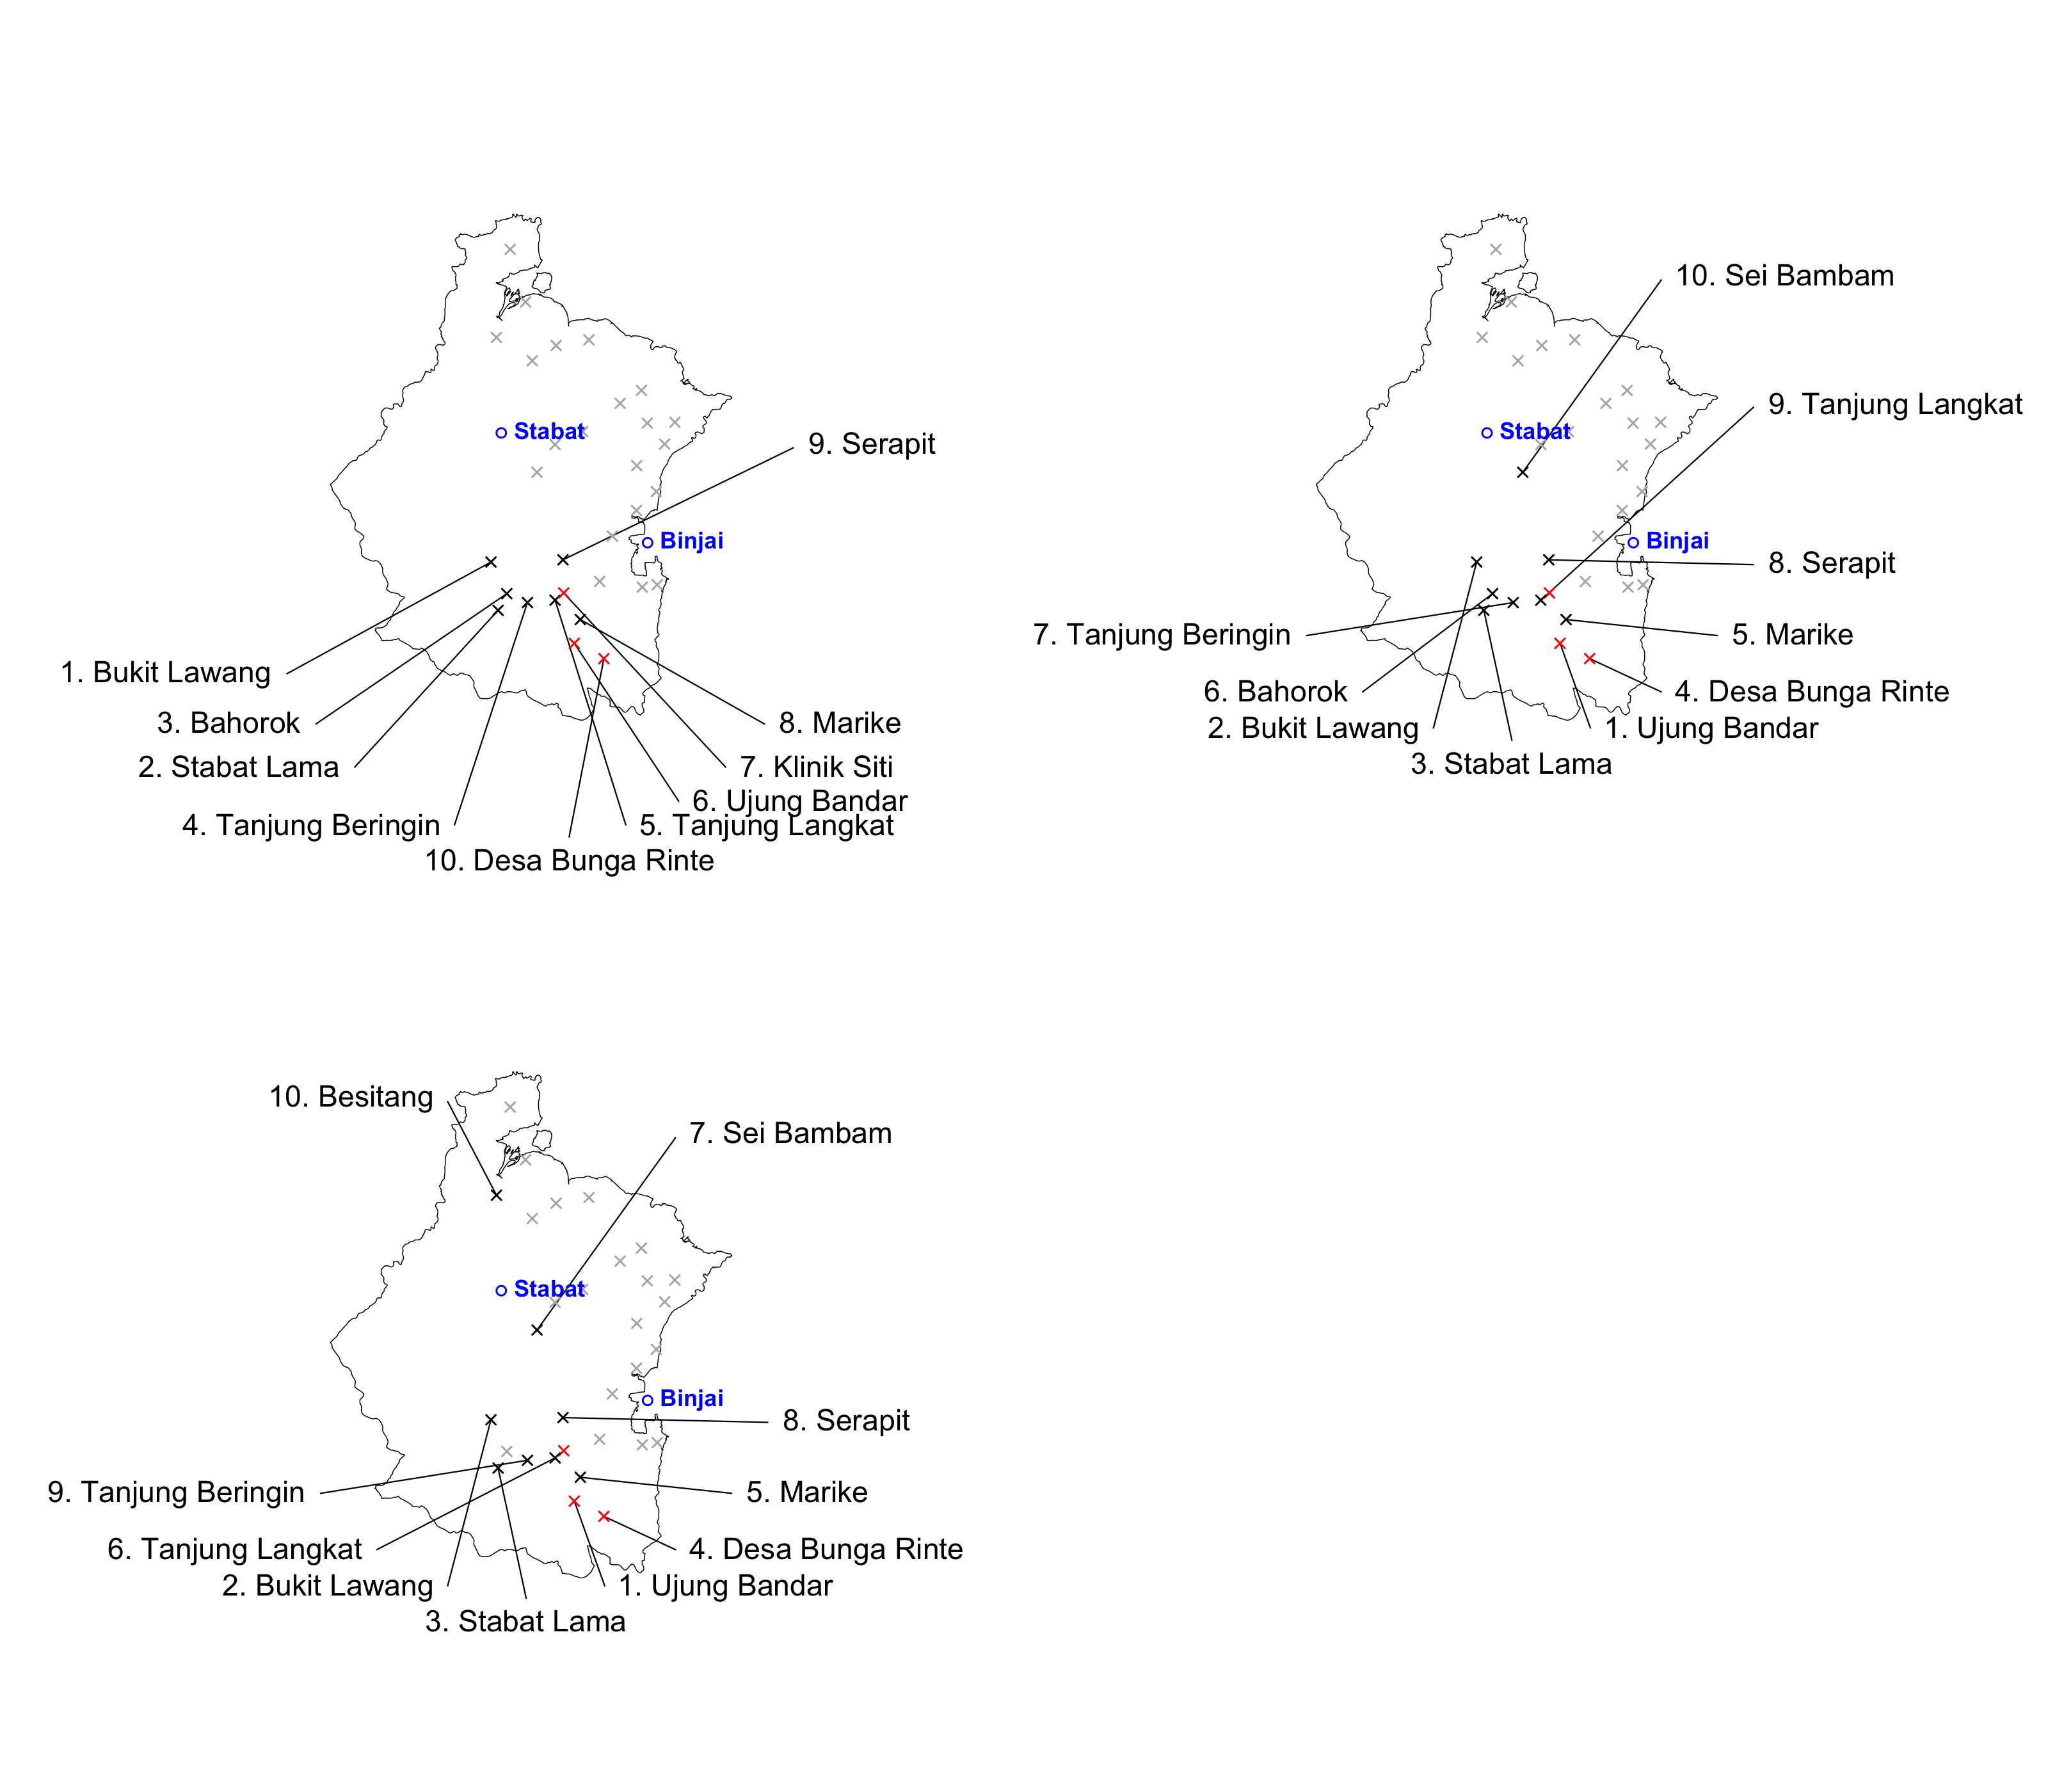
\includegraphics[width=\textwidth]{figs/langkat_all_rank_map.png}
\caption{Mapped best ranked sites in Langkat using catchment definitions of (a) distance-based 
  limits of 30 km (Table \ref{tab:langkat_dist}); (b) travel time-based limits of 100 
  minutes (Table \ref{tab:langkat_time}); and (c) tesselated catchments (Table 
  \ref{tab:langkat_stretch}). Site with ranks shaded in grey were suggested by surveillance study stakeholders. 
 Eco-constraints are indicated in green (pass) and purple (fail), summarised as ``Eco-constraints Present''.}
\label{fig:maps_langkat}
\end{figure}
\clearpage
\subsubsection{Pakpak Bharat}
% latex table generated in R 4.3.1 by xtable 1.8-4 package
% Wed Sep  4 16:11:51 2024
\begin{table}[ht]
\centering
\begingroup\fontsize{8pt}{9pt}\selectfont
\begin{tabular}{C{0.03\textwidth}C{0.12\textwidth}C{0.09\textwidth}C{0.08\textwidth}C{0.08\textwidth}C{0.08\textwidth}C{0.07\textwidth}C{0.07\textwidth}C{0.07\textwidth}C{0.07\textwidth}}
 Rank & Name & Catchment Size & Objective Mean & Objective Std Dev & Eco-constraints  Present & Human Pop & Croplands & Oil Palm & Forest Loss \\ 
 {1} & Sibagindar & 132 & \cellcolor[HTML]{BD0026}\textcolor[HTML]{FFFFFF}{1.04} & \cellcolor[HTML]{FEB24C}\textcolor[HTML]{000000}{0.44} & \cellcolor[HTML]{FD8D3C}\textcolor[HTML]{000000}{4} & \cellcolor[HTML]{90EE90}{******} & \cellcolor[HTML]{90EE90}{ 1.00} & \cellcolor[HTML]{90EE90}{37} & \cellcolor[HTML]{90EE90}{0.29} \\ 
  {2} & Kecupak & 130 & \cellcolor[HTML]{E31A1C}\textcolor[HTML]{FFFFFF}{1.01} & \cellcolor[HTML]{FC4E2A}\textcolor[HTML]{000000}{0.46} & \cellcolor[HTML]{FD8D3C}\textcolor[HTML]{000000}{4} & \cellcolor[HTML]{90EE90}{******} & \cellcolor[HTML]{90EE90}{ 3.99} & \cellcolor[HTML]{90EE90}{37} & \cellcolor[HTML]{90EE90}{0.07} \\ 
  {3} & Singgabur & 132 & \cellcolor[HTML]{E31A1C}\textcolor[HTML]{FFFFFF}{0.98} & \cellcolor[HTML]{FED976}\textcolor[HTML]{000000}{0.42} & \cellcolor[HTML]{FD8D3C}\textcolor[HTML]{000000}{4} & \cellcolor[HTML]{90EE90}{******} & \cellcolor[HTML]{90EE90}{ 3.99} & \cellcolor[HTML]{90EE90}{37} & \cellcolor[HTML]{90EE90}{0.05} \\ 
  {4} & Salak & 134 & \cellcolor[HTML]{E31A1C}\textcolor[HTML]{FFFFFF}{0.98} & \cellcolor[HTML]{FC4E2A}\textcolor[HTML]{000000}{0.46} & \cellcolor[HTML]{FD8D3C}\textcolor[HTML]{000000}{4} & \cellcolor[HTML]{90EE90}{******} & \cellcolor[HTML]{90EE90}{ 3.99} & \cellcolor[HTML]{90EE90}{37} & \cellcolor[HTML]{90EE90}{0.07} \\ 
  {5} & Siempat Rube & 133 & \cellcolor[HTML]{FC4E2A}\textcolor[HTML]{000000}{0.95} & \cellcolor[HTML]{FEB24C}\textcolor[HTML]{000000}{0.44} & \cellcolor[HTML]{FD8D3C}\textcolor[HTML]{000000}{4} & \cellcolor[HTML]{90EE90}{******} & \cellcolor[HTML]{90EE90}{ 3.99} & \cellcolor[HTML]{90EE90}{37} & \cellcolor[HTML]{90EE90}{0.05} \\ 
  {6} & Tinada & 132 & \cellcolor[HTML]{FD8D3C}\textcolor[HTML]{000000}{0.93} & \cellcolor[HTML]{FC4E2A}\textcolor[HTML]{000000}{0.46} & \cellcolor[HTML]{FD8D3C}\textcolor[HTML]{000000}{4} & \cellcolor[HTML]{90EE90}{******} & \cellcolor[HTML]{90EE90}{11.96} & \cellcolor[HTML]{90EE90}{37} & \cellcolor[HTML]{90EE90}{0.07} \\ 
  {7} & Sukaramai & 132 & \cellcolor[HTML]{FED976}\textcolor[HTML]{000000}{0.88} & \cellcolor[HTML]{E31A1C}\textcolor[HTML]{FFFFFF}{0.47} & \cellcolor[HTML]{FD8D3C}\textcolor[HTML]{000000}{4} & \cellcolor[HTML]{90EE90}{******} & \cellcolor[HTML]{90EE90}{11.96} & \cellcolor[HTML]{90EE90}{37} & \cellcolor[HTML]{90EE90}{0.07} \\ 
  {8} & Sibande & 132 & \cellcolor[HTML]{FED976}\textcolor[HTML]{000000}{0.86} & \cellcolor[HTML]{BD0026}\textcolor[HTML]{FFFFFF}{0.50} & \cellcolor[HTML]{FD8D3C}\textcolor[HTML]{000000}{4} & \cellcolor[HTML]{90EE90}{******} & \cellcolor[HTML]{90EE90}{11.96} & \cellcolor[HTML]{90EE90}{37} & \cellcolor[HTML]{90EE90}{0.28} \\ 
  \end{tabular}
\endgroup
\caption{Pakpak Bharat sites (distance catchments, 30 km)} 
\label{tab:pakpak_bharat_dist}
\end{table}
% latex table generated in R 4.3.1 by xtable 1.8-4 package
% Wed Sep  4 16:11:51 2024
\begin{table}[ht]
\centering
\begingroup\fontsize{8pt}{9pt}\selectfont
\begin{tabular}{C{0.03\textwidth}C{0.12\textwidth}C{0.09\textwidth}C{0.08\textwidth}C{0.08\textwidth}C{0.08\textwidth}C{0.07\textwidth}C{0.07\textwidth}C{0.07\textwidth}C{0.07\textwidth}}
 Rank & Name & Catchment Size & Objective Mean & Objective Std Dev & Eco-constraints  Present & Human Pop & Croplands & Oil Palm & Forest Loss \\ 
 {1} & Sibagindar &   5 & \cellcolor[HTML]{BD0026}\textcolor[HTML]{FFFFFF}{1.32} & \cellcolor[HTML]{FED976}\textcolor[HTML]{000000}{0.33} & \cellcolor[HTML]{FED976}\textcolor[HTML]{000000}{2} & \cellcolor[HTML]{9370D8}{****} & \cellcolor[HTML]{9370D8}{ 0.00} & \cellcolor[HTML]{90EE90}{33.14} & \cellcolor[HTML]{90EE90}{0.05} \\ 
  {2} & Singgabur & 108 & \cellcolor[HTML]{FED976}\textcolor[HTML]{000000}{0.67} & \cellcolor[HTML]{BD0026}\textcolor[HTML]{FFFFFF}{0.49} & \cellcolor[HTML]{BD0026}\textcolor[HTML]{FFFFFF}{4} & \cellcolor[HTML]{90EE90}{******} & \cellcolor[HTML]{90EE90}{11.96} & \cellcolor[HTML]{90EE90}{37.00} & \cellcolor[HTML]{90EE90}{0.08} \\ 
  {3} & Tinada & 220 & \cellcolor[HTML]{FED976}\textcolor[HTML]{000000}{0.63} & \cellcolor[HTML]{E31A1C}\textcolor[HTML]{FFFFFF}{0.45} & \cellcolor[HTML]{BD0026}\textcolor[HTML]{FFFFFF}{4} & \cellcolor[HTML]{90EE90}{******} & \cellcolor[HTML]{90EE90}{19.94} & \cellcolor[HTML]{90EE90}{37.00} & \cellcolor[HTML]{90EE90}{0.13} \\ 
  {4} & Siempat Rube & 195 & \cellcolor[HTML]{FED976}\textcolor[HTML]{000000}{0.63} & \cellcolor[HTML]{E31A1C}\textcolor[HTML]{FFFFFF}{0.46} & \cellcolor[HTML]{BD0026}\textcolor[HTML]{FFFFFF}{4} & \cellcolor[HTML]{90EE90}{******} & \cellcolor[HTML]{90EE90}{19.94} & \cellcolor[HTML]{90EE90}{37.00} & \cellcolor[HTML]{90EE90}{0.13} \\ 
  {5} & Kecupak & 141 & \cellcolor[HTML]{FED976}\textcolor[HTML]{000000}{0.62} & \cellcolor[HTML]{BD0026}\textcolor[HTML]{FFFFFF}{0.46} & \cellcolor[HTML]{BD0026}\textcolor[HTML]{FFFFFF}{4} & \cellcolor[HTML]{90EE90}{******} & \cellcolor[HTML]{90EE90}{17.96} & \cellcolor[HTML]{90EE90}{37.00} & \cellcolor[HTML]{90EE90}{0.13} \\ 
  {6} & Sibande & 248 & \cellcolor[HTML]{FED976}\textcolor[HTML]{000000}{0.62} & \cellcolor[HTML]{E31A1C}\textcolor[HTML]{FFFFFF}{0.46} & \cellcolor[HTML]{BD0026}\textcolor[HTML]{FFFFFF}{4} & \cellcolor[HTML]{90EE90}{*******} & \cellcolor[HTML]{90EE90}{61.91} & \cellcolor[HTML]{90EE90}{37.00} & \cellcolor[HTML]{90EE90}{0.23} \\ 
  {7} & Salak & 190 & \cellcolor[HTML]{FED976}\textcolor[HTML]{000000}{0.62} & \cellcolor[HTML]{E31A1C}\textcolor[HTML]{FFFFFF}{0.45} & \cellcolor[HTML]{BD0026}\textcolor[HTML]{FFFFFF}{4} & \cellcolor[HTML]{90EE90}{******} & \cellcolor[HTML]{90EE90}{19.94} & \cellcolor[HTML]{90EE90}{37.00} & \cellcolor[HTML]{90EE90}{0.13} \\ 
  {8} & Sukaramai & 266 & \cellcolor[HTML]{FED976}\textcolor[HTML]{000000}{0.60} & \cellcolor[HTML]{E31A1C}\textcolor[HTML]{FFFFFF}{0.46} & \cellcolor[HTML]{BD0026}\textcolor[HTML]{FFFFFF}{4} & \cellcolor[HTML]{90EE90}{*******} & \cellcolor[HTML]{90EE90}{61.91} & \cellcolor[HTML]{90EE90}{37.00} & \cellcolor[HTML]{90EE90}{0.13} \\ 
  \end{tabular}
\endgroup
\caption{Pakpak Bharat sites (travel time catchments, 100 minutes)} 
\label{tab:pakpak_bharat_time}
\end{table}
% latex table generated in R 4.3.1 by xtable 1.8-4 package
% Wed Sep  4 16:11:51 2024
\begin{table}[ht]
\centering
\begingroup\fontsize{8pt}{9pt}\selectfont
\begin{tabular}{C{0.03\textwidth}C{0.12\textwidth}C{0.09\textwidth}C{0.08\textwidth}C{0.08\textwidth}C{0.08\textwidth}C{0.07\textwidth}C{0.07\textwidth}C{0.07\textwidth}C{0.07\textwidth}}
 Rank & Name & Catchment Size & Objective Mean & Objective Std Dev & Eco-constraints  Present & Human Pop & Croplands & Oil Palm & Forest Loss \\ 
 {1} & Sibagindar &  20 & \cellcolor[HTML]{BD0026}\textcolor[HTML]{FFFFFF}{1.31} & \cellcolor[HTML]{FD8D3C}\textcolor[HTML]{000000}{0.34} & \cellcolor[HTML]{FD8D3C}\textcolor[HTML]{000000}{2} & \cellcolor[HTML]{9370D8}{****} & \cellcolor[HTML]{9370D8}{0} & \cellcolor[HTML]{90EE90}{33.14} & \cellcolor[HTML]{90EE90}{0.05} \\ 
  {2} & Kecupak &   6 & \cellcolor[HTML]{BD0026}\textcolor[HTML]{FFFFFF}{1.29} & \cellcolor[HTML]{FEB24C}\textcolor[HTML]{000000}{0.34} & \cellcolor[HTML]{FD8D3C}\textcolor[HTML]{000000}{2} & \cellcolor[HTML]{9370D8}{****} & \cellcolor[HTML]{9370D8}{0} & \cellcolor[HTML]{90EE90}{ 9.27} & \cellcolor[HTML]{90EE90}{0.02} \\ 
  {3} & Tinada &   3 & \cellcolor[HTML]{FC4E2A}\textcolor[HTML]{000000}{1.15} & \cellcolor[HTML]{E31A1C}\textcolor[HTML]{FFFFFF}{0.45} & \cellcolor[HTML]{FD8D3C}\textcolor[HTML]{000000}{2} & \cellcolor[HTML]{9370D8}{****} & \cellcolor[HTML]{9370D8}{0} & \cellcolor[HTML]{90EE90}{36.72} & \cellcolor[HTML]{90EE90}{0.03} \\ 
  {4} & Sibande &  15 & \cellcolor[HTML]{FC4E2A}\textcolor[HTML]{000000}{1.14} & \cellcolor[HTML]{BD0026}\textcolor[HTML]{FFFFFF}{0.55} & \cellcolor[HTML]{FD8D3C}\textcolor[HTML]{000000}{2} & \cellcolor[HTML]{9370D8}{****} & \cellcolor[HTML]{9370D8}{0} & \cellcolor[HTML]{90EE90}{29.15} & \cellcolor[HTML]{90EE90}{0.03} \\ 
  {5} & Singgabur &   7 & \cellcolor[HTML]{FC4E2A}\textcolor[HTML]{000000}{1.13} & \cellcolor[HTML]{FD8D3C}\textcolor[HTML]{000000}{0.37} & \cellcolor[HTML]{FD8D3C}\textcolor[HTML]{000000}{2} & \cellcolor[HTML]{9370D8}{****} & \cellcolor[HTML]{9370D8}{0} & \cellcolor[HTML]{90EE90}{31.45} & \cellcolor[HTML]{90EE90}{0.01} \\ 
  {6} & Sukaramai &   4 & \cellcolor[HTML]{FEB24C}\textcolor[HTML]{000000}{0.96} & \cellcolor[HTML]{FED976}\textcolor[HTML]{000000}{0.24} & \cellcolor[HTML]{FD8D3C}\textcolor[HTML]{000000}{2} & \cellcolor[HTML]{9370D8}{****} & \cellcolor[HTML]{9370D8}{0} & \cellcolor[HTML]{90EE90}{35.38} & \cellcolor[HTML]{90EE90}{0.02} \\ 
  {7} & Siempat Rube &   3 & \cellcolor[HTML]{FED976}\textcolor[HTML]{000000}{0.89} & \cellcolor[HTML]{FED976}\textcolor[HTML]{000000}{0.27} & \cellcolor[HTML]{FD8D3C}\textcolor[HTML]{000000}{2} & \cellcolor[HTML]{9370D8}{****} & \cellcolor[HTML]{9370D8}{0} & \cellcolor[HTML]{90EE90}{37.00} & \cellcolor[HTML]{90EE90}{0.03} \\ 
  {8} & Salak &   2 & \cellcolor[HTML]{FED976}\textcolor[HTML]{000000}{0.86} & \cellcolor[HTML]{FEB24C}\textcolor[HTML]{000000}{0.30} & \cellcolor[HTML]{FD8D3C}\textcolor[HTML]{000000}{2} & \cellcolor[HTML]{9370D8}{****} & \cellcolor[HTML]{9370D8}{0} & \cellcolor[HTML]{90EE90}{27.04} & \cellcolor[HTML]{90EE90}{0.02} \\ 
  \end{tabular}
\endgroup
\caption{Pakpak Bharat sites (``closest point'' catchments)} 
\label{tab:pakpak_bharat_stretch}
\end{table}
\begin{figure}
\centering
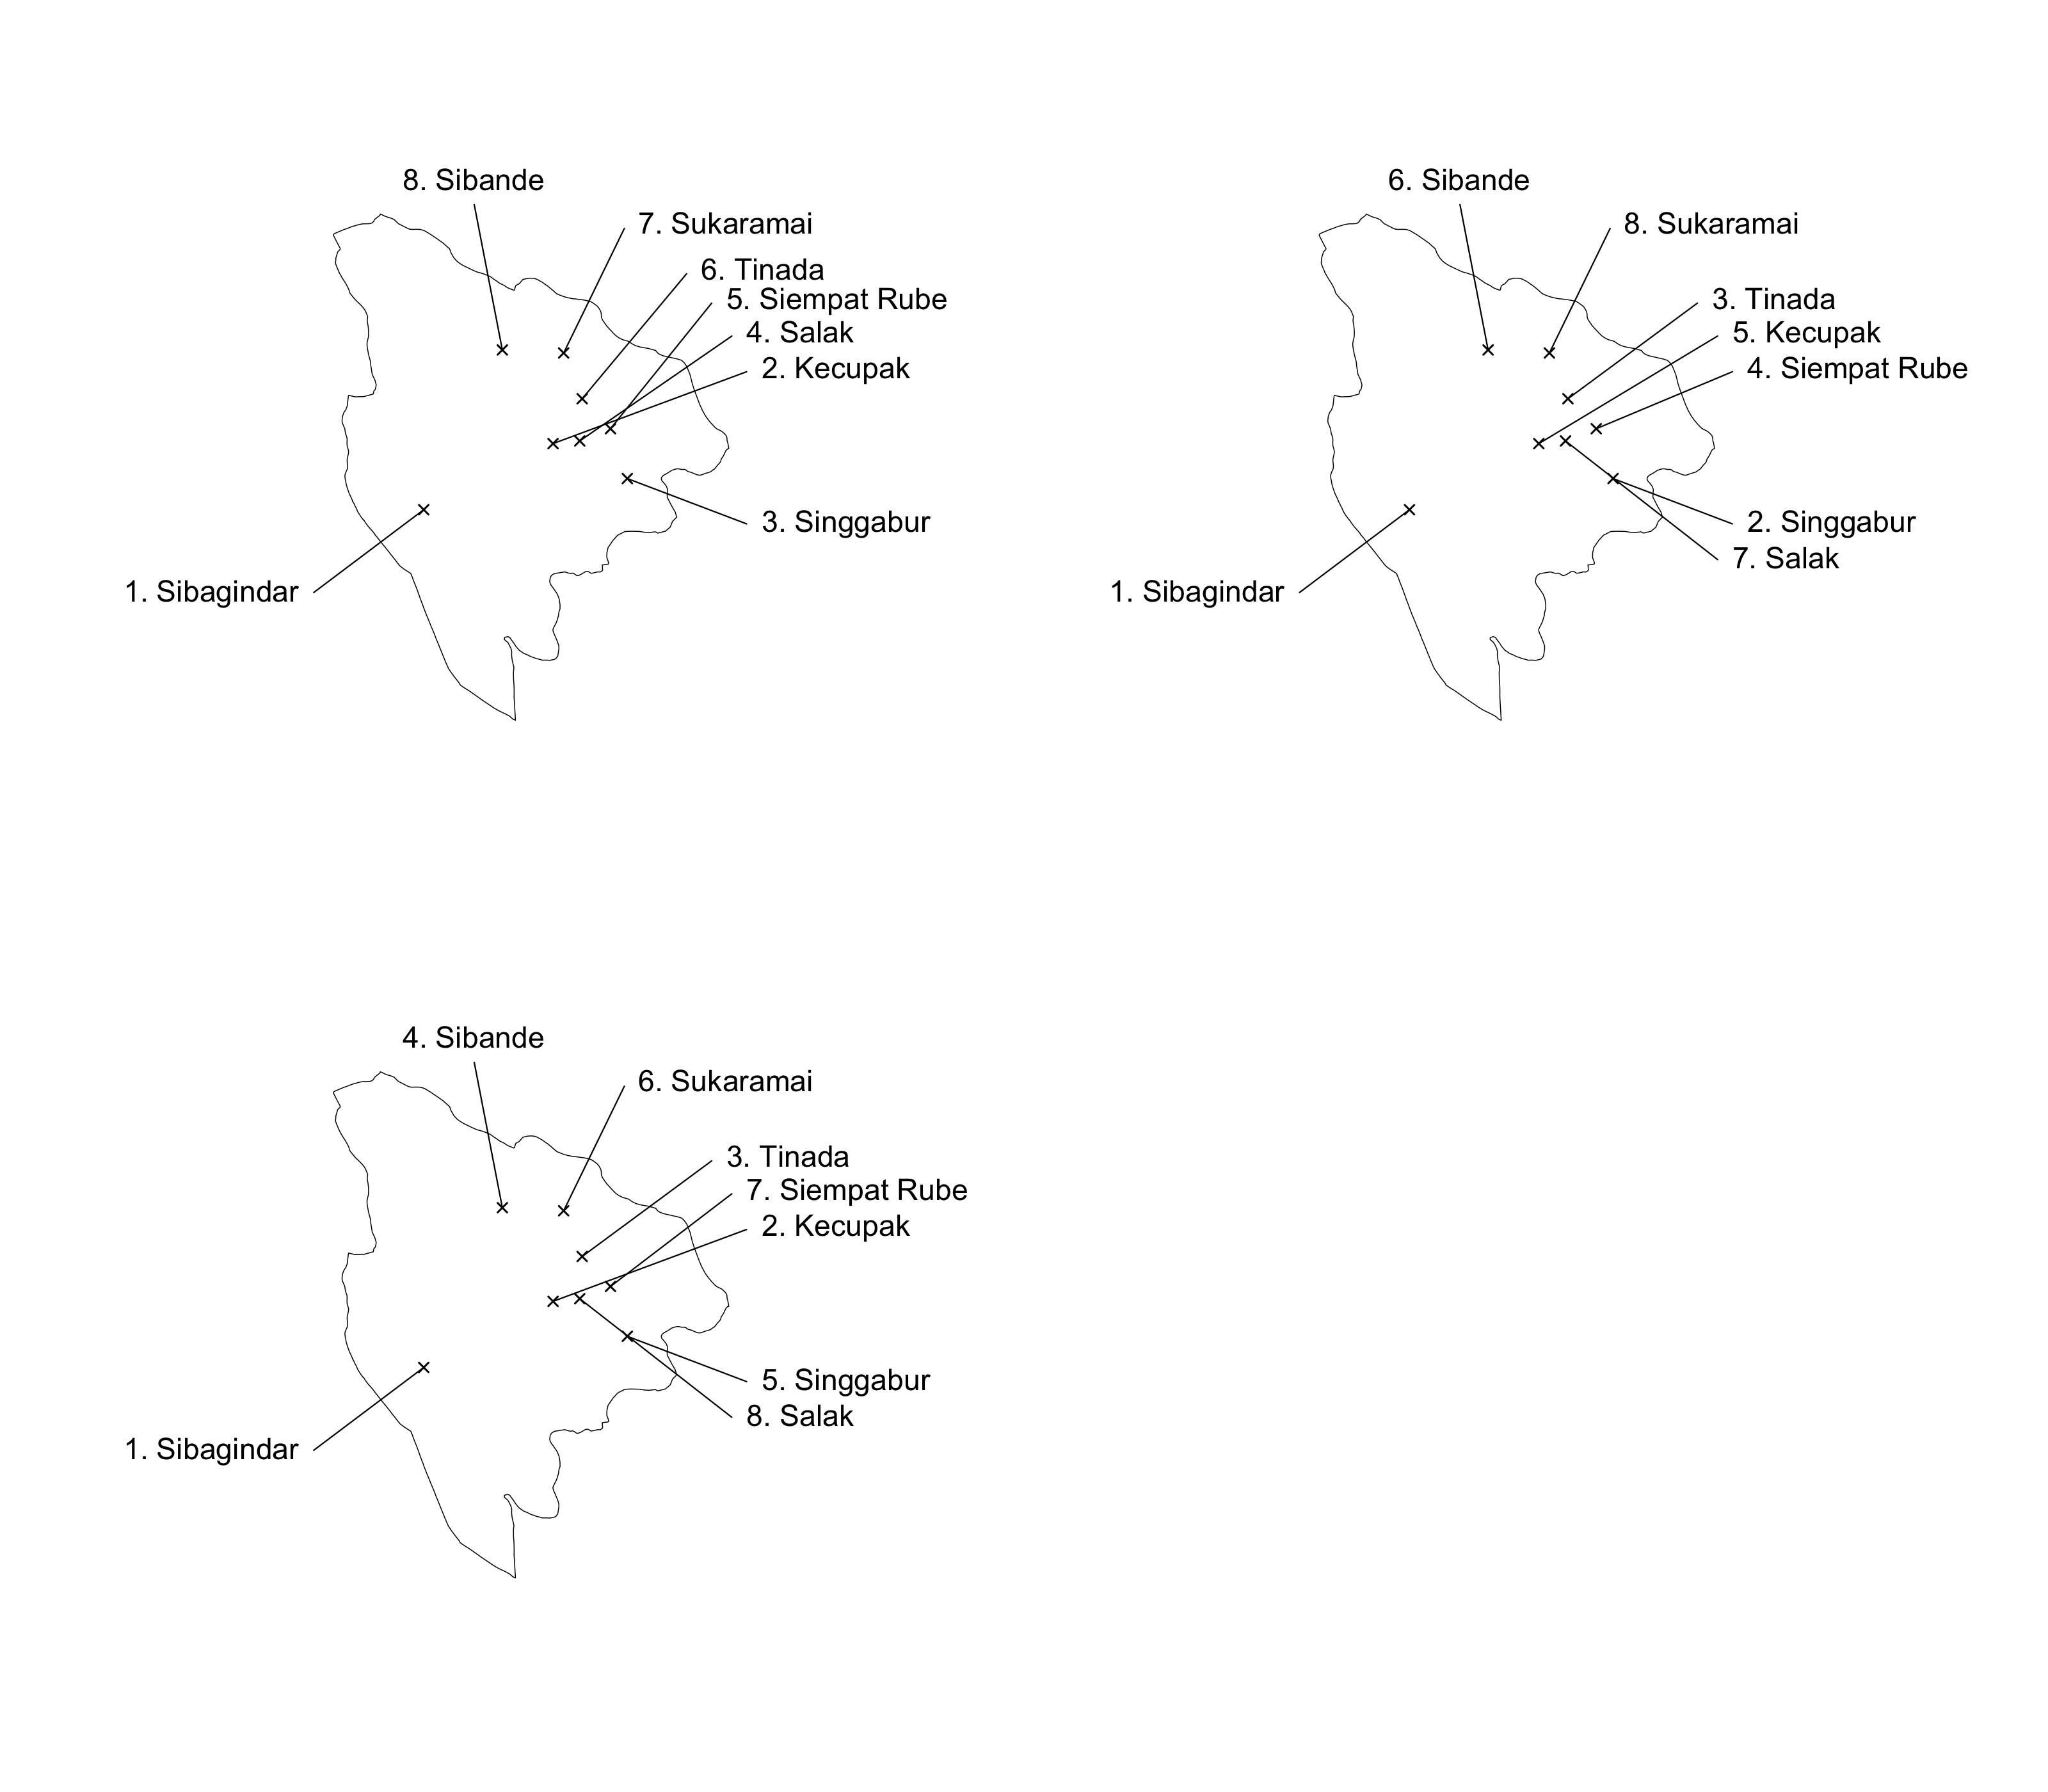
\includegraphics[width=\textwidth]{figs/pakpak_bharat_all_rank_map.png}
\caption{Mapped best ranked sites in Pakpak Bharat using catchment definitions of (a) distance-based 
  limits of 30 km (Table \ref{tab:pakpak_bharat_dist}); (b) travel time-based limits of 100 
  minutes (Table \ref{tab:pakpak_bharat_time}); and (c) tesselated catchments (Table 
  \ref{tab:pakpak_bharat_stretch}). Site with ranks shaded in grey were suggested by surveillance study stakeholders. 
 Eco-constraints are indicated in green (pass) and purple (fail), summarised as ``Eco-constraints Present''.}
\label{fig:maps_pakpak_bharat}
\end{figure}
\clearpage
\subsubsection{Malinau}
% latex table generated in R 4.3.1 by xtable 1.8-4 package
% Wed Sep  4 16:11:51 2024
\begin{table}[ht]
\centering
\begingroup\fontsize{8pt}{9pt}\selectfont
\begin{tabular}{C{0.03\textwidth}C{0.12\textwidth}C{0.09\textwidth}C{0.08\textwidth}C{0.08\textwidth}C{0.08\textwidth}C{0.07\textwidth}C{0.07\textwidth}C{0.07\textwidth}C{0.07\textwidth}}
 Rank & Name & Catchment Size & Objective Mean & Objective Std Dev & Eco-constraints  Present & Human Pop & Croplands & Oil Palm & Forest Loss \\ 
 {1} & Sungaiboh & 114 & \cellcolor[HTML]{BD0026}\textcolor[HTML]{FFFFFF}{1.49} & \cellcolor[HTML]{E31A1C}\textcolor[HTML]{FFFFFF}{0.32} & \cellcolor[HTML]{FD8D3C}\textcolor[HTML]{000000}{2} & \cellcolor[HTML]{9370D8}{****} & \cellcolor[HTML]{9370D8}{0} & \cellcolor[HTML]{90EE90}{20.68} & \cellcolor[HTML]{90EE90}{0.06} \\ 
  {2} & Longampung & 117 & \cellcolor[HTML]{BD0026}\textcolor[HTML]{FFFFFF}{1.41} & \cellcolor[HTML]{FD8D3C}\textcolor[HTML]{000000}{0.28} & \cellcolor[HTML]{BD0026}\textcolor[HTML]{FFFFFF}{3} & \cellcolor[HTML]{90EE90}{*****} & \cellcolor[HTML]{9370D8}{0} & \cellcolor[HTML]{90EE90}{21.80} & \cellcolor[HTML]{90EE90}{0.05} \\ 
  {3} & Longnawang &  96 & \cellcolor[HTML]{E31A1C}\textcolor[HTML]{FFFFFF}{1.35} & \cellcolor[HTML]{FEB24C}\textcolor[HTML]{000000}{0.26} & \cellcolor[HTML]{BD0026}\textcolor[HTML]{FFFFFF}{3} & \cellcolor[HTML]{90EE90}{*****} & \cellcolor[HTML]{9370D8}{0} & \cellcolor[HTML]{90EE90}{21.80} & \cellcolor[HTML]{90EE90}{0.09} \\ 
  {4} & Longberang & 113 & \cellcolor[HTML]{E31A1C}\textcolor[HTML]{FFFFFF}{1.32} & \cellcolor[HTML]{BD0026}\textcolor[HTML]{FFFFFF}{0.36} & \cellcolor[HTML]{FED976}\textcolor[HTML]{000000}{1} & \cellcolor[HTML]{9370D8}{****} & \cellcolor[HTML]{9370D8}{0} & \cellcolor[HTML]{9370D8}{ 0.00} & \cellcolor[HTML]{90EE90}{0.01} \\ 
  {5} & Longsule & 115 & \cellcolor[HTML]{E31A1C}\textcolor[HTML]{FFFFFF}{1.31} & \cellcolor[HTML]{FED976}\textcolor[HTML]{000000}{0.23} & \cellcolor[HTML]{FD8D3C}\textcolor[HTML]{000000}{2} & \cellcolor[HTML]{9370D8}{****} & \cellcolor[HTML]{9370D8}{0} & \cellcolor[HTML]{90EE90}{20.68} & \cellcolor[HTML]{90EE90}{0.04} \\ 
  {6} & Longalango & 103 & \cellcolor[HTML]{FC4E2A}\textcolor[HTML]{000000}{1.27} & \cellcolor[HTML]{FC4E2A}\textcolor[HTML]{000000}{0.29} & \cellcolor[HTML]{BD0026}\textcolor[HTML]{FFFFFF}{3} & \cellcolor[HTML]{90EE90}{*****} & \cellcolor[HTML]{9370D8}{0} & \cellcolor[HTML]{90EE90}{26.82} & \cellcolor[HTML]{90EE90}{0.02} \\ 
  {7} & Longloreh & 111 & \cellcolor[HTML]{FC4E2A}\textcolor[HTML]{000000}{1.24} & \cellcolor[HTML]{FEB24C}\textcolor[HTML]{000000}{0.24} & \cellcolor[HTML]{FD8D3C}\textcolor[HTML]{000000}{2} & \cellcolor[HTML]{9370D8}{****} & \cellcolor[HTML]{9370D8}{0} & \cellcolor[HTML]{90EE90}{26.57} & \cellcolor[HTML]{90EE90}{0.14} \\ 
  {8} & Sehati & 112 & \cellcolor[HTML]{FD8D3C}\textcolor[HTML]{000000}{1.16} & \cellcolor[HTML]{FED976}\textcolor[HTML]{000000}{0.21} & \cellcolor[HTML]{BD0026}\textcolor[HTML]{FFFFFF}{3} & \cellcolor[HTML]{90EE90}{*****} & \cellcolor[HTML]{9370D8}{0} & \cellcolor[HTML]{90EE90}{36.50} & \cellcolor[HTML]{90EE90}{0.14} \\ 
  \cellcolor{lightgray}{9} & Pulau Sapi & 114 & \cellcolor[HTML]{FD8D3C}\textcolor[HTML]{000000}{1.16} & \cellcolor[HTML]{FC4E2A}\textcolor[HTML]{000000}{0.29} & \cellcolor[HTML]{BD0026}\textcolor[HTML]{FFFFFF}{3} & \cellcolor[HTML]{90EE90}{*****} & \cellcolor[HTML]{9370D8}{0} & \cellcolor[HTML]{90EE90}{37.00} & \cellcolor[HTML]{90EE90}{0.13} \\ 
  {10} & Setulang & 116 & \cellcolor[HTML]{FD8D3C}\textcolor[HTML]{000000}{1.15} & \cellcolor[HTML]{FEB24C}\textcolor[HTML]{000000}{0.26} & \cellcolor[HTML]{BD0026}\textcolor[HTML]{FFFFFF}{3} & \cellcolor[HTML]{90EE90}{*****} & \cellcolor[HTML]{9370D8}{0} & \cellcolor[HTML]{90EE90}{37.00} & \cellcolor[HTML]{90EE90}{0.13} \\ 
  {-} & Tanjunglapang & 114 & \cellcolor[HTML]{FD8D3C}\textcolor[HTML]{000000}{1.10} & \cellcolor[HTML]{FC4E2A}\textcolor[HTML]{000000}{0.30} & \cellcolor[HTML]{BD0026}\textcolor[HTML]{FFFFFF}{3} & \cellcolor[HTML]{90EE90}{*****} & \cellcolor[HTML]{9370D8}{0} & \cellcolor[HTML]{90EE90}{37.00} & \cellcolor[HTML]{90EE90}{0.17} \\ 
  {-} & Sesua & 115 & \cellcolor[HTML]{FD8D3C}\textcolor[HTML]{000000}{1.10} & \cellcolor[HTML]{FC4E2A}\textcolor[HTML]{000000}{0.29} & \cellcolor[HTML]{BD0026}\textcolor[HTML]{FFFFFF}{3} & \cellcolor[HTML]{90EE90}{*****} & \cellcolor[HTML]{9370D8}{0} & \cellcolor[HTML]{90EE90}{37.00} & \cellcolor[HTML]{90EE90}{0.17} \\ 
  \cellcolor{lightgray}{-} & RSUD Malinau & 114 & \cellcolor[HTML]{FD8D3C}\textcolor[HTML]{000000}{1.09} & \cellcolor[HTML]{E31A1C}\textcolor[HTML]{FFFFFF}{0.32} & \cellcolor[HTML]{BD0026}\textcolor[HTML]{FFFFFF}{3} & \cellcolor[HTML]{90EE90}{*****} & \cellcolor[HTML]{9370D8}{0} & \cellcolor[HTML]{90EE90}{37.00} & \cellcolor[HTML]{90EE90}{0.17} \\ 
  \cellcolor{lightgray}{-} & Malinau Kota & 116 & \cellcolor[HTML]{FD8D3C}\textcolor[HTML]{000000}{1.08} & \cellcolor[HTML]{E31A1C}\textcolor[HTML]{FFFFFF}{0.32} & \cellcolor[HTML]{BD0026}\textcolor[HTML]{FFFFFF}{3} & \cellcolor[HTML]{90EE90}{*****} & \cellcolor[HTML]{9370D8}{0} & \cellcolor[HTML]{90EE90}{37.00} & \cellcolor[HTML]{90EE90}{0.17} \\ 
  \cellcolor{lightgray}{-} & Sekatak & 111 & \cellcolor[HTML]{FED976}\textcolor[HTML]{000000}{0.87} & \cellcolor[HTML]{E31A1C}\textcolor[HTML]{FFFFFF}{0.33} & \cellcolor[HTML]{BD0026}\textcolor[HTML]{FFFFFF}{3} & \cellcolor[HTML]{90EE90}{*****} & \cellcolor[HTML]{9370D8}{0} & \cellcolor[HTML]{90EE90}{35.17} & \cellcolor[HTML]{90EE90}{0.25} \\ 
  \end{tabular}
\endgroup
\caption{Malinau sites (distance catchments, 30 km)} 
\label{tab:malinau_dist}
\end{table}
% latex table generated in R 4.3.1 by xtable 1.8-4 package
% Wed Sep  4 16:11:51 2024
\begin{table}[ht]
\centering
\begingroup\fontsize{8pt}{9pt}\selectfont
\begin{tabular}{C{0.03\textwidth}C{0.12\textwidth}C{0.09\textwidth}C{0.08\textwidth}C{0.08\textwidth}C{0.08\textwidth}C{0.07\textwidth}C{0.07\textwidth}C{0.07\textwidth}C{0.07\textwidth}}
 Rank & Name & Catchment Size & Objective Mean & Objective Std Dev & Eco-constraints  Present & Human Pop & Croplands & Oil Palm & Forest Loss \\ 
 {1} & Sungaiboh &  48 & \cellcolor[HTML]{BD0026}\textcolor[HTML]{FFFFFF}{1.51} & \cellcolor[HTML]{FD8D3C}\textcolor[HTML]{000000}{0.27} & \cellcolor[HTML]{FEB24C}\textcolor[HTML]{000000}{1} & \cellcolor[HTML]{9370D8}{****} & \cellcolor[HTML]{9370D8}{0} & \cellcolor[HTML]{9370D8}{ 0.00} & \cellcolor[HTML]{90EE90}{0.01} \\ 
  {2} & Longampung &  46 & \cellcolor[HTML]{BD0026}\textcolor[HTML]{FFFFFF}{1.47} & \cellcolor[HTML]{FC4E2A}\textcolor[HTML]{000000}{0.31} & \cellcolor[HTML]{FC4E2A}\textcolor[HTML]{000000}{2} & \cellcolor[HTML]{9370D8}{****} & \cellcolor[HTML]{9370D8}{0} & \cellcolor[HTML]{90EE90}{20.68} & \cellcolor[HTML]{90EE90}{0.05} \\ 
  {3} & Longalango &  18 & \cellcolor[HTML]{FC4E2A}\textcolor[HTML]{000000}{1.25} & \cellcolor[HTML]{BD0026}\textcolor[HTML]{FFFFFF}{0.39} & \cellcolor[HTML]{FC4E2A}\textcolor[HTML]{000000}{2} & \cellcolor[HTML]{9370D8}{****} & \cellcolor[HTML]{9370D8}{0} & \cellcolor[HTML]{90EE90}{26.82} & \cellcolor[HTML]{90EE90}{0.01} \\ 
  {4} & Longnawang &  14 & \cellcolor[HTML]{FD8D3C}\textcolor[HTML]{000000}{1.21} & \cellcolor[HTML]{FED976}\textcolor[HTML]{000000}{0.20} & \cellcolor[HTML]{FC4E2A}\textcolor[HTML]{000000}{2} & \cellcolor[HTML]{9370D8}{****} & \cellcolor[HTML]{9370D8}{0} & \cellcolor[HTML]{90EE90}{21.80} & \cellcolor[HTML]{90EE90}{0.09} \\ 
  {5} & Longloreh &  16 & \cellcolor[HTML]{FD8D3C}\textcolor[HTML]{000000}{1.19} & \cellcolor[HTML]{FEB24C}\textcolor[HTML]{000000}{0.24} & \cellcolor[HTML]{FC4E2A}\textcolor[HTML]{000000}{2} & \cellcolor[HTML]{9370D8}{****} & \cellcolor[HTML]{9370D8}{0} & \cellcolor[HTML]{90EE90}{26.57} & \cellcolor[HTML]{90EE90}{0.14} \\ 
  {6} & Longsule &   1 & \cellcolor[HTML]{FD8D3C}\textcolor[HTML]{000000}{1.16} & \cellcolor[HTML]{FFFFFF}\textcolor[HTML]{000000}{  NA} & \cellcolor[HTML]{FED976}\textcolor[HTML]{000000}{0} & \cellcolor[HTML]{9370D8}{**} & \cellcolor[HTML]{9370D8}{0} & \cellcolor[HTML]{9370D8}{ 0.00} & \cellcolor[HTML]{9370D8}{0.00} \\ 
  \cellcolor{lightgray}{7} & Pulau Sapi & 166 & \cellcolor[HTML]{FEB24C}\textcolor[HTML]{000000}{1.05} & \cellcolor[HTML]{FC4E2A}\textcolor[HTML]{000000}{0.32} & \cellcolor[HTML]{BD0026}\textcolor[HTML]{FFFFFF}{3} & \cellcolor[HTML]{90EE90}{*****} & \cellcolor[HTML]{9370D8}{0} & \cellcolor[HTML]{90EE90}{37.00} & \cellcolor[HTML]{90EE90}{0.19} \\ 
  {8} & Setulang & 120 & \cellcolor[HTML]{FED976}\textcolor[HTML]{000000}{1.05} & \cellcolor[HTML]{FC4E2A}\textcolor[HTML]{000000}{0.31} & \cellcolor[HTML]{BD0026}\textcolor[HTML]{FFFFFF}{3} & \cellcolor[HTML]{90EE90}{*****} & \cellcolor[HTML]{9370D8}{0} & \cellcolor[HTML]{90EE90}{37.00} & \cellcolor[HTML]{90EE90}{0.19} \\ 
  {9} & Tanjunglapang & 202 & \cellcolor[HTML]{FED976}\textcolor[HTML]{000000}{1.04} & \cellcolor[HTML]{E31A1C}\textcolor[HTML]{FFFFFF}{0.35} & \cellcolor[HTML]{BD0026}\textcolor[HTML]{FFFFFF}{3} & \cellcolor[HTML]{90EE90}{*****} & \cellcolor[HTML]{9370D8}{0} & \cellcolor[HTML]{90EE90}{37.00} & \cellcolor[HTML]{90EE90}{0.19} \\ 
  {10} & Sesua & 203 & \cellcolor[HTML]{FED976}\textcolor[HTML]{000000}{1.04} & \cellcolor[HTML]{E31A1C}\textcolor[HTML]{FFFFFF}{0.35} & \cellcolor[HTML]{BD0026}\textcolor[HTML]{FFFFFF}{3} & \cellcolor[HTML]{90EE90}{*****} & \cellcolor[HTML]{9370D8}{0} & \cellcolor[HTML]{90EE90}{37.00} & \cellcolor[HTML]{90EE90}{0.19} \\ 
  {-} & Longberang &   1 & \cellcolor[HTML]{FED976}\textcolor[HTML]{000000}{1.03} & \cellcolor[HTML]{FFFFFF}\textcolor[HTML]{000000}{  NA} & \cellcolor[HTML]{FEB24C}\textcolor[HTML]{000000}{1} & \cellcolor[HTML]{9370D8}{**} & \cellcolor[HTML]{9370D8}{0} & \cellcolor[HTML]{9370D8}{ 0.00} & \cellcolor[HTML]{90EE90}{0.01} \\ 
  {-} & Sehati &  43 & \cellcolor[HTML]{FED976}\textcolor[HTML]{000000}{1.03} & \cellcolor[HTML]{FC4E2A}\textcolor[HTML]{000000}{0.32} & \cellcolor[HTML]{BD0026}\textcolor[HTML]{FFFFFF}{3} & \cellcolor[HTML]{90EE90}{*****} & \cellcolor[HTML]{9370D8}{0} & \cellcolor[HTML]{90EE90}{37.00} & \cellcolor[HTML]{90EE90}{0.14} \\ 
  \cellcolor{lightgray}{-} & RSUD Malinau & 215 & \cellcolor[HTML]{FED976}\textcolor[HTML]{000000}{1.02} & \cellcolor[HTML]{E31A1C}\textcolor[HTML]{FFFFFF}{0.35} & \cellcolor[HTML]{BD0026}\textcolor[HTML]{FFFFFF}{3} & \cellcolor[HTML]{90EE90}{******} & \cellcolor[HTML]{9370D8}{0} & \cellcolor[HTML]{90EE90}{37.00} & \cellcolor[HTML]{90EE90}{0.19} \\ 
  \cellcolor{lightgray}{-} & Malinau Kota & 224 & \cellcolor[HTML]{FED976}\textcolor[HTML]{000000}{1.02} & \cellcolor[HTML]{E31A1C}\textcolor[HTML]{FFFFFF}{0.35} & \cellcolor[HTML]{BD0026}\textcolor[HTML]{FFFFFF}{3} & \cellcolor[HTML]{90EE90}{******} & \cellcolor[HTML]{9370D8}{0} & \cellcolor[HTML]{90EE90}{37.00} & \cellcolor[HTML]{90EE90}{0.25} \\ 
  \cellcolor{lightgray}{-} & Sekatak & 226 & \cellcolor[HTML]{FED976}\textcolor[HTML]{000000}{0.96} & \cellcolor[HTML]{E31A1C}\textcolor[HTML]{FFFFFF}{0.33} & \cellcolor[HTML]{BD0026}\textcolor[HTML]{FFFFFF}{3} & \cellcolor[HTML]{90EE90}{******} & \cellcolor[HTML]{9370D8}{0} & \cellcolor[HTML]{90EE90}{37.00} & \cellcolor[HTML]{90EE90}{0.25} \\ 
  \end{tabular}
\endgroup
\caption{Malinau sites (travel time catchments, 100 minutes)} 
\label{tab:malinau_time}
\end{table}
% latex table generated in R 4.3.1 by xtable 1.8-4 package
% Wed Sep  4 16:11:51 2024
\begin{table}[ht]
\centering
\begingroup\fontsize{8pt}{9pt}\selectfont
\begin{tabular}{C{0.03\textwidth}C{0.12\textwidth}C{0.09\textwidth}C{0.08\textwidth}C{0.08\textwidth}C{0.08\textwidth}C{0.07\textwidth}C{0.07\textwidth}C{0.07\textwidth}C{0.07\textwidth}}
 Rank & Name & Catchment Size & Objective Mean & Objective Std Dev & Eco-constraints  Present & Human Pop & Croplands & Oil Palm & Forest Loss \\ 
 {1} & Sungaiboh & 199 & \cellcolor[HTML]{BD0026}\textcolor[HTML]{FFFFFF}{1.49} & \cellcolor[HTML]{E31A1C}\textcolor[HTML]{FFFFFF}{0.34} & \cellcolor[HTML]{BD0026}\textcolor[HTML]{FFFFFF}{3} & \cellcolor[HTML]{90EE90}{*****} & \cellcolor[HTML]{9370D8}{0} & \cellcolor[HTML]{90EE90}{13.26} & \cellcolor[HTML]{90EE90}{0.06} \\ 
  {2} & Longampung &  99 & \cellcolor[HTML]{BD0026}\textcolor[HTML]{FFFFFF}{1.41} & \cellcolor[HTML]{FC4E2A}\textcolor[HTML]{000000}{0.30} & \cellcolor[HTML]{FED976}\textcolor[HTML]{000000}{2} & \cellcolor[HTML]{9370D8}{****} & \cellcolor[HTML]{9370D8}{0} & \cellcolor[HTML]{90EE90}{20.68} & \cellcolor[HTML]{90EE90}{0.04} \\ 
  {3} & Longnawang & 157 & \cellcolor[HTML]{E31A1C}\textcolor[HTML]{FFFFFF}{1.37} & \cellcolor[HTML]{FD8D3C}\textcolor[HTML]{000000}{0.26} & \cellcolor[HTML]{BD0026}\textcolor[HTML]{FFFFFF}{3} & \cellcolor[HTML]{90EE90}{*****} & \cellcolor[HTML]{9370D8}{0} & \cellcolor[HTML]{90EE90}{21.80} & \cellcolor[HTML]{90EE90}{0.09} \\ 
  {4} & Longberang & 141 & \cellcolor[HTML]{E31A1C}\textcolor[HTML]{FFFFFF}{1.34} & \cellcolor[HTML]{BD0026}\textcolor[HTML]{FFFFFF}{0.36} & \cellcolor[HTML]{FED976}\textcolor[HTML]{000000}{2} & \cellcolor[HTML]{9370D8}{****} & \cellcolor[HTML]{9370D8}{0} & \cellcolor[HTML]{90EE90}{10.03} & \cellcolor[HTML]{90EE90}{0.01} \\ 
  {5} & Longalango & 334 & \cellcolor[HTML]{E31A1C}\textcolor[HTML]{FFFFFF}{1.31} & \cellcolor[HTML]{FEB24C}\textcolor[HTML]{000000}{0.22} & \cellcolor[HTML]{BD0026}\textcolor[HTML]{FFFFFF}{3} & \cellcolor[HTML]{90EE90}{*****} & \cellcolor[HTML]{9370D8}{0} & \cellcolor[HTML]{90EE90}{13.37} & \cellcolor[HTML]{90EE90}{0.05} \\ 
  {6} & Longsule & 543 & \cellcolor[HTML]{E31A1C}\textcolor[HTML]{FFFFFF}{1.30} & \cellcolor[HTML]{FED976}\textcolor[HTML]{000000}{0.19} & \cellcolor[HTML]{BD0026}\textcolor[HTML]{FFFFFF}{3} & \cellcolor[HTML]{90EE90}{*****} & \cellcolor[HTML]{9370D8}{0} & \cellcolor[HTML]{90EE90}{ 5.76} & \cellcolor[HTML]{90EE90}{0.01} \\ 
  {7} & Longloreh & 463 & \cellcolor[HTML]{FC4E2A}\textcolor[HTML]{000000}{1.24} & \cellcolor[HTML]{E31A1C}\textcolor[HTML]{FFFFFF}{0.32} & \cellcolor[HTML]{BD0026}\textcolor[HTML]{FFFFFF}{3} & \cellcolor[HTML]{90EE90}{*****} & \cellcolor[HTML]{9370D8}{0} & \cellcolor[HTML]{90EE90}{31.90} & \cellcolor[HTML]{90EE90}{0.14} \\ 
  \cellcolor{lightgray}{8} & Pulau Sapi &  25 & \cellcolor[HTML]{FC4E2A}\textcolor[HTML]{000000}{1.24} & \cellcolor[HTML]{FEB24C}\textcolor[HTML]{000000}{0.21} & \cellcolor[HTML]{FED976}\textcolor[HTML]{000000}{2} & \cellcolor[HTML]{9370D8}{****} & \cellcolor[HTML]{9370D8}{0} & \cellcolor[HTML]{90EE90}{23.77} & \cellcolor[HTML]{90EE90}{0.09} \\ 
  {9} & Setulang &  41 & \cellcolor[HTML]{FC4E2A}\textcolor[HTML]{000000}{1.23} & \cellcolor[HTML]{FD8D3C}\textcolor[HTML]{000000}{0.25} & \cellcolor[HTML]{FED976}\textcolor[HTML]{000000}{2} & \cellcolor[HTML]{9370D8}{****} & \cellcolor[HTML]{9370D8}{0} & \cellcolor[HTML]{90EE90}{21.84} & \cellcolor[HTML]{90EE90}{0.05} \\ 
  {10} & Tanjunglapang &   5 & \cellcolor[HTML]{FD8D3C}\textcolor[HTML]{000000}{1.14} & \cellcolor[HTML]{FD8D3C}\textcolor[HTML]{000000}{0.25} & \cellcolor[HTML]{FED976}\textcolor[HTML]{000000}{2} & \cellcolor[HTML]{9370D8}{****} & \cellcolor[HTML]{9370D8}{0} & \cellcolor[HTML]{90EE90}{31.80} & \cellcolor[HTML]{90EE90}{0.07} \\ 
  {-} & Sehati &  43 & \cellcolor[HTML]{FD8D3C}\textcolor[HTML]{000000}{1.13} & \cellcolor[HTML]{FED976}\textcolor[HTML]{000000}{0.17} & \cellcolor[HTML]{FED976}\textcolor[HTML]{000000}{2} & \cellcolor[HTML]{9370D8}{****} & \cellcolor[HTML]{9370D8}{0} & \cellcolor[HTML]{90EE90}{18.54} & \cellcolor[HTML]{90EE90}{0.05} \\ 
  \cellcolor{lightgray}{-} & RSUD Malinau &  14 & \cellcolor[HTML]{FD8D3C}\textcolor[HTML]{000000}{1.13} & \cellcolor[HTML]{FEB24C}\textcolor[HTML]{000000}{0.21} & \cellcolor[HTML]{FED976}\textcolor[HTML]{000000}{2} & \cellcolor[HTML]{9370D8}{****} & \cellcolor[HTML]{9370D8}{0} & \cellcolor[HTML]{90EE90}{33.55} & \cellcolor[HTML]{90EE90}{0.10} \\ 
  {-} & Sesua &   7 & \cellcolor[HTML]{FED976}\textcolor[HTML]{000000}{0.91} & \cellcolor[HTML]{E31A1C}\textcolor[HTML]{FFFFFF}{0.34} & \cellcolor[HTML]{FED976}\textcolor[HTML]{000000}{2} & \cellcolor[HTML]{9370D8}{****} & \cellcolor[HTML]{9370D8}{0} & \cellcolor[HTML]{90EE90}{36.50} & \cellcolor[HTML]{90EE90}{0.05} \\ 
  \cellcolor{lightgray}{-} & Malinau Kota &  12 & \cellcolor[HTML]{FED976}\textcolor[HTML]{000000}{0.90} & \cellcolor[HTML]{BD0026}\textcolor[HTML]{FFFFFF}{0.38} & \cellcolor[HTML]{FED976}\textcolor[HTML]{000000}{2} & \cellcolor[HTML]{9370D8}{****} & \cellcolor[HTML]{9370D8}{0} & \cellcolor[HTML]{90EE90}{37.00} & \cellcolor[HTML]{90EE90}{0.08} \\ 
  \cellcolor{lightgray}{-} & Sekatak & 390 & \cellcolor[HTML]{FED976}\textcolor[HTML]{000000}{0.83} & \cellcolor[HTML]{BD0026}\textcolor[HTML]{FFFFFF}{0.37} & \cellcolor[HTML]{BD0026}\textcolor[HTML]{FFFFFF}{3} & \cellcolor[HTML]{90EE90}{******} & \cellcolor[HTML]{9370D8}{0} & \cellcolor[HTML]{90EE90}{36.92} & \cellcolor[HTML]{90EE90}{0.33} \\ 
  \end{tabular}
\endgroup
\caption{Malinau sites (``closest point'' catchments)} 
\label{tab:malinau_stretch}
\end{table}
\begin{figure}
\centering
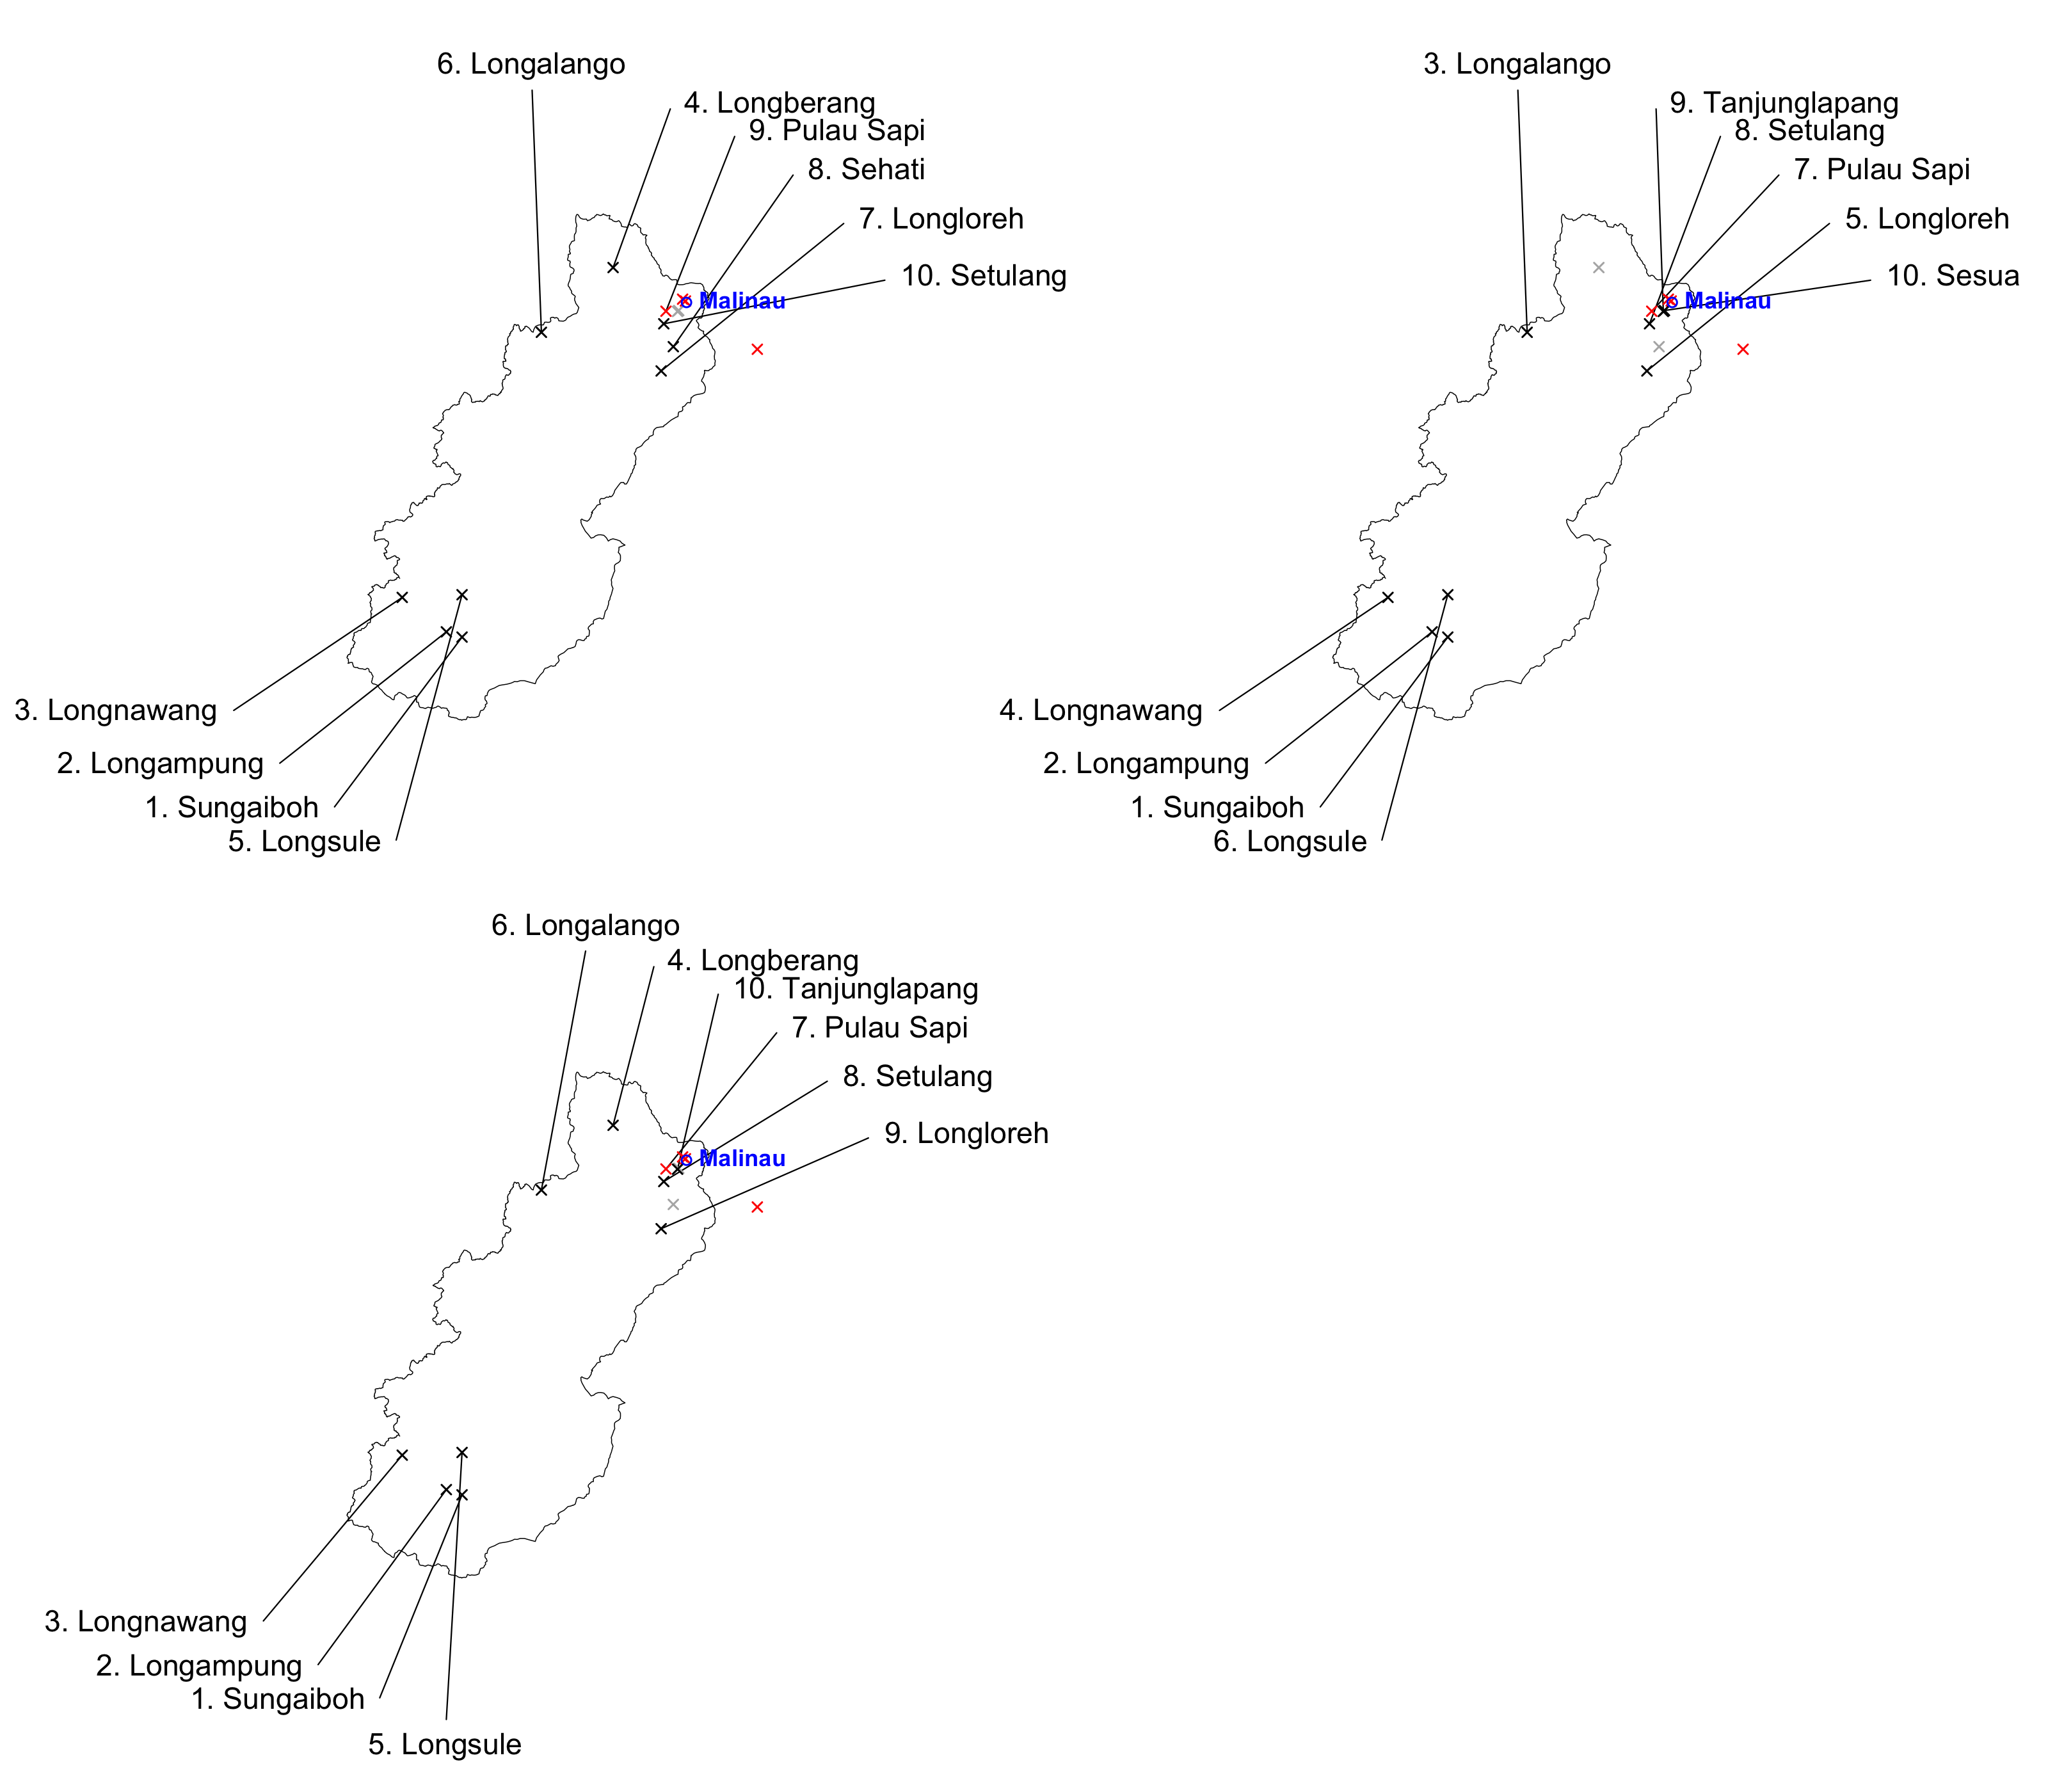
\includegraphics[width=\textwidth]{figs/malinau_all_rank_map.png}
\caption{Mapped best ranked sites in Malinau using catchment definitions of (a) distance-based 
  limits of 30 km (Table \ref{tab:malinau_dist}); (b) travel time-based limits of 100 
  minutes (Table \ref{tab:malinau_time}); and (c) tesselated catchments (Table 
  \ref{tab:malinau_stretch}). Site with ranks shaded in grey were suggested by surveillance study stakeholders. 
 Eco-constraints are indicated in green (pass) and purple (fail), summarised as ``Eco-constraints Present''.}
\label{fig:maps_malinau}
\end{figure}
\clearpage
\subsubsection{Nunukan}
% latex table generated in R 4.3.1 by xtable 1.8-4 package
% Wed Sep  4 16:11:51 2024
\begin{table}[ht]
\centering
\begingroup\fontsize{8pt}{9pt}\selectfont
\begin{tabular}{C{0.03\textwidth}C{0.12\textwidth}C{0.09\textwidth}C{0.08\textwidth}C{0.08\textwidth}C{0.08\textwidth}C{0.07\textwidth}C{0.07\textwidth}C{0.07\textwidth}C{0.07\textwidth}}
 Rank & Name & Catchment Size & Objective Mean & Objective Std Dev & Eco-constraints  Present & Human Pop & Croplands & Oil Palm & Forest Loss \\ 
 {1} & Binter & 101 & \cellcolor[HTML]{BD0026}\textcolor[HTML]{FFFFFF}{1.33} & \cellcolor[HTML]{FC4E2A}\textcolor[HTML]{000000}{0.36} & \cellcolor[HTML]{FED976}\textcolor[HTML]{000000}{2} & \cellcolor[HTML]{9370D8}{****} & \cellcolor[HTML]{9370D8}{0.00} & \cellcolor[HTML]{90EE90}{ 6.88} & \cellcolor[HTML]{90EE90}{0.02} \\ 
  {2} & Long Layu &  87 & \cellcolor[HTML]{E31A1C}\textcolor[HTML]{FFFFFF}{1.09} & \cellcolor[HTML]{FC4E2A}\textcolor[HTML]{000000}{0.34} & \cellcolor[HTML]{FD8D3C}\textcolor[HTML]{000000}{3} & \cellcolor[HTML]{90EE90}{*****} & \cellcolor[HTML]{9370D8}{0.00} & \cellcolor[HTML]{90EE90}{37.00} & \cellcolor[HTML]{90EE90}{0.02} \\ 
  {3} & Aji Kuning & 102 & \cellcolor[HTML]{FC4E2A}\textcolor[HTML]{000000}{1.00} & \cellcolor[HTML]{BD0026}\textcolor[HTML]{FFFFFF}{0.46} & \cellcolor[HTML]{FD8D3C}\textcolor[HTML]{000000}{3} & \cellcolor[HTML]{90EE90}{*****} & \cellcolor[HTML]{9370D8}{0.00} & \cellcolor[HTML]{90EE90}{36.75} & \cellcolor[HTML]{90EE90}{0.27} \\ 
  {4} & Atap & 113 & \cellcolor[HTML]{FC4E2A}\textcolor[HTML]{000000}{0.99} & \cellcolor[HTML]{E31A1C}\textcolor[HTML]{FFFFFF}{0.38} & \cellcolor[HTML]{FD8D3C}\textcolor[HTML]{000000}{3} & \cellcolor[HTML]{90EE90}{*****} & \cellcolor[HTML]{9370D8}{0.00} & \cellcolor[HTML]{90EE90}{35.17} & \cellcolor[HTML]{90EE90}{0.19} \\ 
  {5} & Long Bawan &  80 & \cellcolor[HTML]{FC4E2A}\textcolor[HTML]{000000}{0.99} & \cellcolor[HTML]{FC4E2A}\textcolor[HTML]{000000}{0.33} & \cellcolor[HTML]{FD8D3C}\textcolor[HTML]{000000}{3} & \cellcolor[HTML]{90EE90}{*****} & \cellcolor[HTML]{9370D8}{0.00} & \cellcolor[HTML]{90EE90}{37.00} & \cellcolor[HTML]{90EE90}{0.03} \\ 
  {6} & Sungai Nyamuk & 104 & \cellcolor[HTML]{FC4E2A}\textcolor[HTML]{000000}{0.97} & \cellcolor[HTML]{BD0026}\textcolor[HTML]{FFFFFF}{0.45} & \cellcolor[HTML]{FD8D3C}\textcolor[HTML]{000000}{3} & \cellcolor[HTML]{90EE90}{*****} & \cellcolor[HTML]{9370D8}{0.00} & \cellcolor[HTML]{90EE90}{36.75} & \cellcolor[HTML]{90EE90}{0.15} \\ 
  {7} & Seimenggaris & 103 & \cellcolor[HTML]{FC4E2A}\textcolor[HTML]{000000}{0.94} & \cellcolor[HTML]{BD0026}\textcolor[HTML]{FFFFFF}{0.42} & \cellcolor[HTML]{FD8D3C}\textcolor[HTML]{000000}{3} & \cellcolor[HTML]{90EE90}{*****} & \cellcolor[HTML]{9370D8}{0.00} & \cellcolor[HTML]{90EE90}{36.75} & \cellcolor[HTML]{90EE90}{0.15} \\ 
  {8} & Mansalong & 116 & \cellcolor[HTML]{FC4E2A}\textcolor[HTML]{000000}{0.94} & \cellcolor[HTML]{FC4E2A}\textcolor[HTML]{000000}{0.35} & \cellcolor[HTML]{FD8D3C}\textcolor[HTML]{000000}{3} & \cellcolor[HTML]{90EE90}{*****} & \cellcolor[HTML]{9370D8}{0.00} & \cellcolor[HTML]{90EE90}{37.00} & \cellcolor[HTML]{90EE90}{0.19} \\ 
  {9} & Sanur & 112 & \cellcolor[HTML]{FD8D3C}\textcolor[HTML]{000000}{0.91} & \cellcolor[HTML]{FC4E2A}\textcolor[HTML]{000000}{0.37} & \cellcolor[HTML]{FD8D3C}\textcolor[HTML]{000000}{3} & \cellcolor[HTML]{90EE90}{*****} & \cellcolor[HTML]{9370D8}{0.00} & \cellcolor[HTML]{90EE90}{36.75} & \cellcolor[HTML]{90EE90}{0.27} \\ 
  {10} & Pembeliangan & 115 & \cellcolor[HTML]{FD8D3C}\textcolor[HTML]{000000}{0.91} & \cellcolor[HTML]{FC4E2A}\textcolor[HTML]{000000}{0.34} & \cellcolor[HTML]{FD8D3C}\textcolor[HTML]{000000}{3} & \cellcolor[HTML]{90EE90}{*****} & \cellcolor[HTML]{9370D8}{0.00} & \cellcolor[HTML]{90EE90}{36.75} & \cellcolor[HTML]{90EE90}{0.24} \\ 
  {-} & Tanjung Harapan & 113 & \cellcolor[HTML]{FD8D3C}\textcolor[HTML]{000000}{0.91} & \cellcolor[HTML]{FC4E2A}\textcolor[HTML]{000000}{0.35} & \cellcolor[HTML]{FD8D3C}\textcolor[HTML]{000000}{3} & \cellcolor[HTML]{90EE90}{*****} & \cellcolor[HTML]{9370D8}{0.00} & \cellcolor[HTML]{90EE90}{35.18} & \cellcolor[HTML]{90EE90}{0.24} \\ 
  {-} & Sedadap &  29 & \cellcolor[HTML]{FED976}\textcolor[HTML]{000000}{0.55} & \cellcolor[HTML]{FED976}\textcolor[HTML]{000000}{0.20} & \cellcolor[HTML]{BD0026}\textcolor[HTML]{FFFFFF}{4} & \cellcolor[HTML]{90EE90}{*****} & \cellcolor[HTML]{90EE90}{4.98} & \cellcolor[HTML]{90EE90}{36.84} & \cellcolor[HTML]{90EE90}{0.02} \\ 
  {-} & Sei Taiwan &  17 & \cellcolor[HTML]{FED976}\textcolor[HTML]{000000}{0.54} & \cellcolor[HTML]{FED976}\textcolor[HTML]{000000}{0.19} & \cellcolor[HTML]{BD0026}\textcolor[HTML]{FFFFFF}{4} & \cellcolor[HTML]{90EE90}{*****} & \cellcolor[HTML]{90EE90}{4.98} & \cellcolor[HTML]{90EE90}{36.84} & \cellcolor[HTML]{90EE90}{0.02} \\ 
  {-} & Setabu &  22 & \cellcolor[HTML]{FED976}\textcolor[HTML]{000000}{0.54} & \cellcolor[HTML]{FED976}\textcolor[HTML]{000000}{0.20} & \cellcolor[HTML]{BD0026}\textcolor[HTML]{FFFFFF}{4} & \cellcolor[HTML]{90EE90}{*****} & \cellcolor[HTML]{90EE90}{4.98} & \cellcolor[HTML]{90EE90}{36.84} & \cellcolor[HTML]{90EE90}{0.02} \\ 
  {-} & Lapri &  19 & \cellcolor[HTML]{FED976}\textcolor[HTML]{000000}{0.53} & \cellcolor[HTML]{FED976}\textcolor[HTML]{000000}{0.21} & \cellcolor[HTML]{BD0026}\textcolor[HTML]{FFFFFF}{4} & \cellcolor[HTML]{90EE90}{*****} & \cellcolor[HTML]{90EE90}{4.98} & \cellcolor[HTML]{90EE90}{36.84} & \cellcolor[HTML]{90EE90}{0.02} \\ 
  \end{tabular}
\endgroup
\caption{Nunukan sites (distance catchments, 30 km)} 
\label{tab:nunukan_dist}
\end{table}
% latex table generated in R 4.3.1 by xtable 1.8-4 package
% Wed Sep  4 16:11:51 2024
\begin{table}[ht]
\centering
\begingroup\fontsize{8pt}{9pt}\selectfont
\begin{tabular}{C{0.03\textwidth}C{0.12\textwidth}C{0.09\textwidth}C{0.08\textwidth}C{0.08\textwidth}C{0.08\textwidth}C{0.07\textwidth}C{0.07\textwidth}C{0.07\textwidth}C{0.07\textwidth}}
 Rank & Name & Catchment Size & Objective Mean & Objective Std Dev & Eco-constraints  Present & Human Pop & Croplands & Oil Palm & Forest Loss \\ 
 {1} & Long Layu &  30 & \cellcolor[HTML]{BD0026}\textcolor[HTML]{FFFFFF}{1.18} & \cellcolor[HTML]{FC4E2A}\textcolor[HTML]{000000}{0.39} & \cellcolor[HTML]{FEB24C}\textcolor[HTML]{000000}{2} & \cellcolor[HTML]{9370D8}{****} & \cellcolor[HTML]{9370D8}{0} & \cellcolor[HTML]{90EE90}{26.82} & \cellcolor[HTML]{90EE90}{0.02} \\ 
  {2} & Mansalong & 219 & \cellcolor[HTML]{E31A1C}\textcolor[HTML]{FFFFFF}{1.01} & \cellcolor[HTML]{FD8D3C}\textcolor[HTML]{000000}{0.37} & \cellcolor[HTML]{FC4E2A}\textcolor[HTML]{000000}{3} & \cellcolor[HTML]{90EE90}{******} & \cellcolor[HTML]{9370D8}{0} & \cellcolor[HTML]{90EE90}{37.00} & \cellcolor[HTML]{90EE90}{0.19} \\ 
  {3} & Binter &   5 & \cellcolor[HTML]{E31A1C}\textcolor[HTML]{FFFFFF}{1.01} & \cellcolor[HTML]{FC4E2A}\textcolor[HTML]{000000}{0.40} & \cellcolor[HTML]{FED976}\textcolor[HTML]{000000}{1} & \cellcolor[HTML]{9370D8}{****} & \cellcolor[HTML]{9370D8}{0} & \cellcolor[HTML]{9370D8}{ 0.00} & \cellcolor[HTML]{90EE90}{0.00} \\ 
  {4} & Tanjung Harapan & 213 & \cellcolor[HTML]{E31A1C}\textcolor[HTML]{FFFFFF}{1.00} & \cellcolor[HTML]{FD8D3C}\textcolor[HTML]{000000}{0.36} & \cellcolor[HTML]{FC4E2A}\textcolor[HTML]{000000}{3} & \cellcolor[HTML]{90EE90}{******} & \cellcolor[HTML]{9370D8}{0} & \cellcolor[HTML]{90EE90}{37.00} & \cellcolor[HTML]{90EE90}{0.19} \\ 
  {5} & Pembeliangan & 180 & \cellcolor[HTML]{E31A1C}\textcolor[HTML]{FFFFFF}{0.97} & \cellcolor[HTML]{FC4E2A}\textcolor[HTML]{000000}{0.37} & \cellcolor[HTML]{FC4E2A}\textcolor[HTML]{000000}{3} & \cellcolor[HTML]{90EE90}{*****} & \cellcolor[HTML]{9370D8}{0} & \cellcolor[HTML]{90EE90}{37.00} & \cellcolor[HTML]{90EE90}{0.19} \\ 
  {6} & Sanur & 186 & \cellcolor[HTML]{E31A1C}\textcolor[HTML]{FFFFFF}{0.97} & \cellcolor[HTML]{FC4E2A}\textcolor[HTML]{000000}{0.38} & \cellcolor[HTML]{FC4E2A}\textcolor[HTML]{000000}{3} & \cellcolor[HTML]{90EE90}{*****} & \cellcolor[HTML]{9370D8}{0} & \cellcolor[HTML]{90EE90}{37.00} & \cellcolor[HTML]{90EE90}{0.19} \\ 
  {7} & Aji Kuning & 169 & \cellcolor[HTML]{E31A1C}\textcolor[HTML]{FFFFFF}{0.95} & \cellcolor[HTML]{FC4E2A}\textcolor[HTML]{000000}{0.38} & \cellcolor[HTML]{FC4E2A}\textcolor[HTML]{000000}{3} & \cellcolor[HTML]{90EE90}{*****} & \cellcolor[HTML]{9370D8}{0} & \cellcolor[HTML]{90EE90}{37.00} & \cellcolor[HTML]{90EE90}{0.19} \\ 
  {8} & Sungai Nyamuk & 110 & \cellcolor[HTML]{E31A1C}\textcolor[HTML]{FFFFFF}{0.95} & \cellcolor[HTML]{FC4E2A}\textcolor[HTML]{000000}{0.42} & \cellcolor[HTML]{FC4E2A}\textcolor[HTML]{000000}{3} & \cellcolor[HTML]{90EE90}{*****} & \cellcolor[HTML]{9370D8}{0} & \cellcolor[HTML]{90EE90}{37.00} & \cellcolor[HTML]{90EE90}{0.19} \\ 
  {9} & Seimenggaris & 133 & \cellcolor[HTML]{E31A1C}\textcolor[HTML]{FFFFFF}{0.94} & \cellcolor[HTML]{FC4E2A}\textcolor[HTML]{000000}{0.40} & \cellcolor[HTML]{FC4E2A}\textcolor[HTML]{000000}{3} & \cellcolor[HTML]{90EE90}{*****} & \cellcolor[HTML]{9370D8}{0} & \cellcolor[HTML]{90EE90}{37.00} & \cellcolor[HTML]{90EE90}{0.19} \\ 
  {10} & Atap &   2 & \cellcolor[HTML]{FC4E2A}\textcolor[HTML]{000000}{0.93} & \cellcolor[HTML]{BD0026}\textcolor[HTML]{FFFFFF}{0.64} & \cellcolor[HTML]{FEB24C}\textcolor[HTML]{000000}{2} & \cellcolor[HTML]{9370D8}{***} & \cellcolor[HTML]{9370D8}{0} & \cellcolor[HTML]{90EE90}{27.59} & \cellcolor[HTML]{90EE90}{0.06} \\ 
  {-} & Long Bawan &   8 & \cellcolor[HTML]{FD8D3C}\textcolor[HTML]{000000}{0.81} & \cellcolor[HTML]{FD8D3C}\textcolor[HTML]{000000}{0.32} & \cellcolor[HTML]{FEB24C}\textcolor[HTML]{000000}{2} & \cellcolor[HTML]{9370D8}{****} & \cellcolor[HTML]{9370D8}{0} & \cellcolor[HTML]{90EE90}{37.00} & \cellcolor[HTML]{90EE90}{0.03} \\ 
  {-} & Setabu &   9 & \cellcolor[HTML]{FEB24C}\textcolor[HTML]{000000}{0.61} & \cellcolor[HTML]{FEB24C}\textcolor[HTML]{000000}{0.19} & \cellcolor[HTML]{FC4E2A}\textcolor[HTML]{000000}{3} & \cellcolor[HTML]{9370D8}{****} & \cellcolor[HTML]{90EE90}{1} & \cellcolor[HTML]{90EE90}{36.84} & \cellcolor[HTML]{90EE90}{0.02} \\ 
  {-} & Sedadap &  10 & \cellcolor[HTML]{FEB24C}\textcolor[HTML]{000000}{0.60} & \cellcolor[HTML]{FED976}\textcolor[HTML]{000000}{0.19} & \cellcolor[HTML]{FC4E2A}\textcolor[HTML]{000000}{3} & \cellcolor[HTML]{9370D8}{****} & \cellcolor[HTML]{90EE90}{1} & \cellcolor[HTML]{90EE90}{36.84} & \cellcolor[HTML]{90EE90}{0.02} \\ 
  {-} & Sei Taiwan &  11 & \cellcolor[HTML]{FED976}\textcolor[HTML]{000000}{0.58} & \cellcolor[HTML]{FEB24C}\textcolor[HTML]{000000}{0.19} & \cellcolor[HTML]{BD0026}\textcolor[HTML]{FFFFFF}{4} & \cellcolor[HTML]{90EE90}{*****} & \cellcolor[HTML]{90EE90}{1} & \cellcolor[HTML]{90EE90}{36.84} & \cellcolor[HTML]{90EE90}{0.02} \\ 
  {-} & Lapri &   7 & \cellcolor[HTML]{FED976}\textcolor[HTML]{000000}{0.46} & \cellcolor[HTML]{FED976}\textcolor[HTML]{000000}{0.10} & \cellcolor[HTML]{FC4E2A}\textcolor[HTML]{000000}{3} & \cellcolor[HTML]{9370D8}{****} & \cellcolor[HTML]{90EE90}{1} & \cellcolor[HTML]{90EE90}{36.84} & \cellcolor[HTML]{90EE90}{0.01} \\ 
  \end{tabular}
\endgroup
\caption{Nunukan sites (travel time catchments, 100 minutes)} 
\label{tab:nunukan_time}
\end{table}
% latex table generated in R 4.3.1 by xtable 1.8-4 package
% Wed Sep  4 16:11:51 2024
\begin{table}[ht]
\centering
\begingroup\fontsize{8pt}{9pt}\selectfont
\begin{tabular}{C{0.03\textwidth}C{0.12\textwidth}C{0.09\textwidth}C{0.08\textwidth}C{0.08\textwidth}C{0.08\textwidth}C{0.07\textwidth}C{0.07\textwidth}C{0.07\textwidth}C{0.07\textwidth}}
 Rank & Name & Catchment Size & Objective Mean & Objective Std Dev & Eco-constraints  Present & Human Pop & Croplands & Oil Palm & Forest Loss \\ 
 {1} & Binter & 114 & \cellcolor[HTML]{BD0026}\textcolor[HTML]{FFFFFF}{1.28} & \cellcolor[HTML]{FC4E2A}\textcolor[HTML]{000000}{0.34} & \cellcolor[HTML]{FED976}\textcolor[HTML]{000000}{2} & \cellcolor[HTML]{90EE90}{*****} & \cellcolor[HTML]{9370D8}{0.00} & \cellcolor[HTML]{9370D8}{ 0.00} & \cellcolor[HTML]{90EE90}{0.02} \\ 
  {2} & Aji Kuning &  60 & \cellcolor[HTML]{BD0026}\textcolor[HTML]{FFFFFF}{1.15} & \cellcolor[HTML]{BD0026}\textcolor[HTML]{FFFFFF}{0.61} & \cellcolor[HTML]{FD8D3C}\textcolor[HTML]{000000}{3} & \cellcolor[HTML]{90EE90}{*****} & \cellcolor[HTML]{9370D8}{0.00} & \cellcolor[HTML]{90EE90}{32.81} & \cellcolor[HTML]{90EE90}{0.27} \\ 
  {3} & Long Layu &  56 & \cellcolor[HTML]{E31A1C}\textcolor[HTML]{FFFFFF}{1.11} & \cellcolor[HTML]{FC4E2A}\textcolor[HTML]{000000}{0.35} & \cellcolor[HTML]{FD8D3C}\textcolor[HTML]{000000}{3} & \cellcolor[HTML]{90EE90}{*****} & \cellcolor[HTML]{9370D8}{0.00} & \cellcolor[HTML]{90EE90}{26.82} & \cellcolor[HTML]{90EE90}{0.02} \\ 
  {4} & Atap &  75 & \cellcolor[HTML]{E31A1C}\textcolor[HTML]{FFFFFF}{1.10} & \cellcolor[HTML]{E31A1C}\textcolor[HTML]{FFFFFF}{0.42} & \cellcolor[HTML]{FD8D3C}\textcolor[HTML]{000000}{3} & \cellcolor[HTML]{90EE90}{*****} & \cellcolor[HTML]{9370D8}{0.00} & \cellcolor[HTML]{90EE90}{31.56} & \cellcolor[HTML]{90EE90}{0.13} \\ 
  {5} & Mansalong &  15 & \cellcolor[HTML]{E31A1C}\textcolor[HTML]{FFFFFF}{1.07} & \cellcolor[HTML]{FC4E2A}\textcolor[HTML]{000000}{0.34} & \cellcolor[HTML]{FED976}\textcolor[HTML]{000000}{2} & \cellcolor[HTML]{9370D8}{****} & \cellcolor[HTML]{9370D8}{0.00} & \cellcolor[HTML]{90EE90}{30.86} & \cellcolor[HTML]{90EE90}{0.17} \\ 
  {6} & Sanur &  15 & \cellcolor[HTML]{E31A1C}\textcolor[HTML]{FFFFFF}{1.03} & \cellcolor[HTML]{FC4E2A}\textcolor[HTML]{000000}{0.33} & \cellcolor[HTML]{FED976}\textcolor[HTML]{000000}{2} & \cellcolor[HTML]{9370D8}{****} & \cellcolor[HTML]{9370D8}{0.00} & \cellcolor[HTML]{90EE90}{35.17} & \cellcolor[HTML]{90EE90}{0.04} \\ 
  {7} & Long Bawan &  74 & \cellcolor[HTML]{E31A1C}\textcolor[HTML]{FFFFFF}{1.01} & \cellcolor[HTML]{FC4E2A}\textcolor[HTML]{000000}{0.34} & \cellcolor[HTML]{FD8D3C}\textcolor[HTML]{000000}{3} & \cellcolor[HTML]{90EE90}{*****} & \cellcolor[HTML]{9370D8}{0.00} & \cellcolor[HTML]{90EE90}{37.00} & \cellcolor[HTML]{90EE90}{0.03} \\ 
  {8} & Seimenggaris &  55 & \cellcolor[HTML]{FC4E2A}\textcolor[HTML]{000000}{0.94} & \cellcolor[HTML]{E31A1C}\textcolor[HTML]{FFFFFF}{0.49} & \cellcolor[HTML]{FD8D3C}\textcolor[HTML]{000000}{3} & \cellcolor[HTML]{90EE90}{*****} & \cellcolor[HTML]{9370D8}{0.00} & \cellcolor[HTML]{90EE90}{35.84} & \cellcolor[HTML]{90EE90}{0.05} \\ 
  {9} & Tanjung Harapan &  32 & \cellcolor[HTML]{FC4E2A}\textcolor[HTML]{000000}{0.88} & \cellcolor[HTML]{FC4E2A}\textcolor[HTML]{000000}{0.31} & \cellcolor[HTML]{FD8D3C}\textcolor[HTML]{000000}{3} & \cellcolor[HTML]{90EE90}{*****} & \cellcolor[HTML]{9370D8}{0.00} & \cellcolor[HTML]{90EE90}{35.10} & \cellcolor[HTML]{90EE90}{0.20} \\ 
  {10} & Pembeliangan &  95 & \cellcolor[HTML]{FD8D3C}\textcolor[HTML]{000000}{0.72} & \cellcolor[HTML]{FD8D3C}\textcolor[HTML]{000000}{0.24} & \cellcolor[HTML]{FD8D3C}\textcolor[HTML]{000000}{3} & \cellcolor[HTML]{90EE90}{*****} & \cellcolor[HTML]{9370D8}{0.00} & \cellcolor[HTML]{90EE90}{36.75} & \cellcolor[HTML]{90EE90}{0.35} \\ 
  {-} & Sedadap &  59 & \cellcolor[HTML]{FEB24C}\textcolor[HTML]{000000}{0.61} & \cellcolor[HTML]{FEB24C}\textcolor[HTML]{000000}{0.20} & \cellcolor[HTML]{BD0026}\textcolor[HTML]{FFFFFF}{4} & \cellcolor[HTML]{90EE90}{*****} & \cellcolor[HTML]{90EE90}{4.98} & \cellcolor[HTML]{90EE90}{36.69} & \cellcolor[HTML]{90EE90}{0.24} \\ 
  {-} & Setabu &   2 & \cellcolor[HTML]{FEB24C}\textcolor[HTML]{000000}{0.52} & \cellcolor[HTML]{FED976}\textcolor[HTML]{000000}{0.02} & \cellcolor[HTML]{FED976}\textcolor[HTML]{000000}{2} & \cellcolor[HTML]{9370D8}{****} & \cellcolor[HTML]{9370D8}{0.00} & \cellcolor[HTML]{90EE90}{35.49} & \cellcolor[HTML]{90EE90}{0.01} \\ 
  {-} & Sei Taiwan &   4 & \cellcolor[HTML]{FEB24C}\textcolor[HTML]{000000}{0.50} & \cellcolor[HTML]{FED976}\textcolor[HTML]{000000}{0.05} & \cellcolor[HTML]{FED976}\textcolor[HTML]{000000}{2} & \cellcolor[HTML]{9370D8}{****} & \cellcolor[HTML]{9370D8}{0.00} & \cellcolor[HTML]{90EE90}{35.81} & \cellcolor[HTML]{90EE90}{0.01} \\ 
  {-} & Sungai Nyamuk &   3 & \cellcolor[HTML]{FED976}\textcolor[HTML]{000000}{0.47} & \cellcolor[HTML]{FD8D3C}\textcolor[HTML]{000000}{0.25} & \cellcolor[HTML]{FED976}\textcolor[HTML]{000000}{2} & \cellcolor[HTML]{9370D8}{****} & \cellcolor[HTML]{9370D8}{0.00} & \cellcolor[HTML]{90EE90}{34.00} & \cellcolor[HTML]{90EE90}{0.06} \\ 
  {-} & Lapri &   2 & \cellcolor[HTML]{FED976}\textcolor[HTML]{000000}{0.33} & \cellcolor[HTML]{FED976}\textcolor[HTML]{000000}{0.06} & \cellcolor[HTML]{FD8D3C}\textcolor[HTML]{000000}{3} & \cellcolor[HTML]{9370D8}{****} & \cellcolor[HTML]{90EE90}{1.00} & \cellcolor[HTML]{90EE90}{36.84} & \cellcolor[HTML]{90EE90}{0.01} \\ 
  \end{tabular}
\endgroup
\caption{Nunukan sites (``closest point'' catchments)} 
\label{tab:nunukan_stretch}
\end{table}
\begin{figure}
\centering
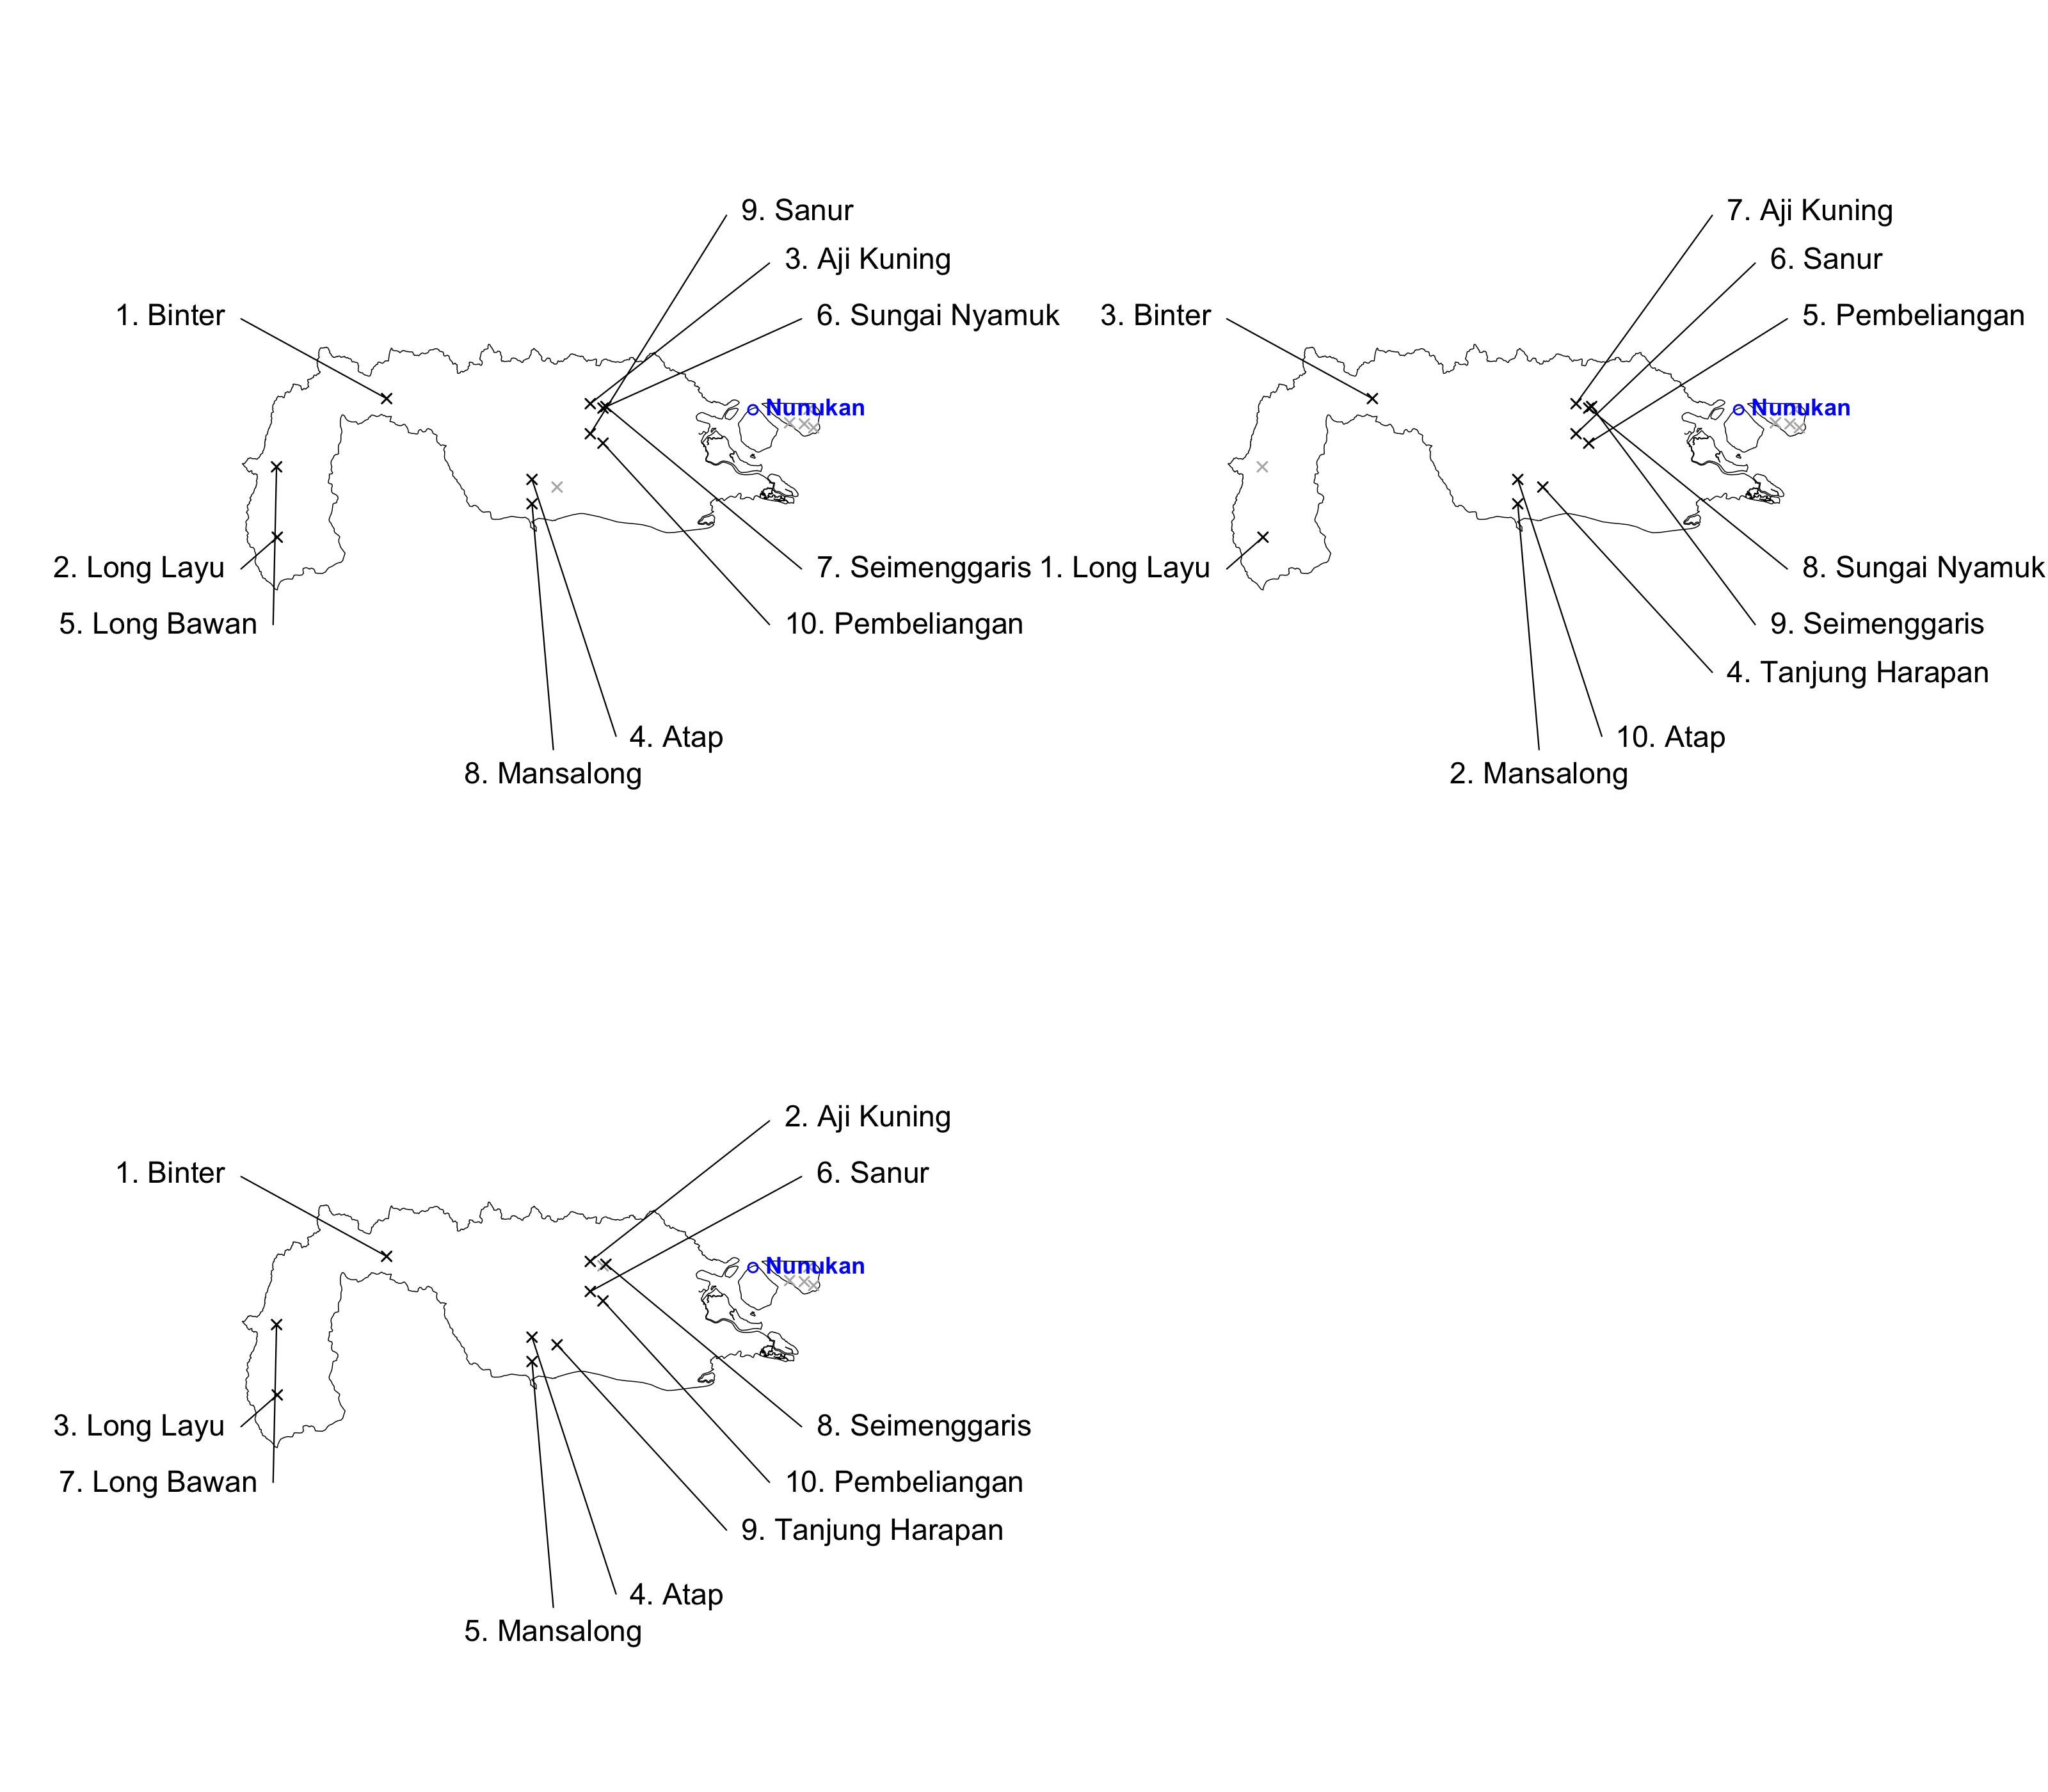
\includegraphics[width=\textwidth]{figs/nunukan_all_rank_map.png}
\caption{Mapped best ranked sites in Nunukan using catchment definitions of (a) distance-based 
  limits of 30 km (Table \ref{tab:nunukan_dist}); (b) travel time-based limits of 100 
  minutes (Table \ref{tab:nunukan_time}); and (c) tesselated catchments (Table 
  \ref{tab:nunukan_stretch}). Site with ranks shaded in grey were suggested by surveillance study stakeholders. 
 Eco-constraints are indicated in green (pass) and purple (fail), summarised as ``Eco-constraints Present''.}
\label{fig:maps_nunukan}
\end{figure}
\clearpage
